\documentclass[english,twoside,openany,showtrims]{sbabook}

\usepackage{url}
\makeatletter
\def\url@leostyle{%
  \@ifundefined{selectfont}{\def\UrlFont{\sf}}{\def\UrlFont{\sffamily}}}
\makeatother
% Now actually use the newly defined style.
\urlstyle{leo}

\usepackage{graphicx}
\def\etc{{\textit{etc}}}
\def\eg{{\textit{e.g.}}}
\def\ie{{\textit{i.e.}}}
\def\cf{{\textit{c.f.}}\ }
\def\erf{\mathop{\textrm{erf}}}
\def\sign{\mathop{\textrm{sign}}}
\def\prob{\mathop{\textrm{Prob}}}
\def\var{\mathop{\textrm{var}}}
\def\mod{\mathop{\textrm{mod}}}
\def\cor{\mathop{\textrm{cor}}}
\def\cov{\mathop{\textrm{cov}}}
\def\cl{\mathop{\textrm{CL}}}
\def\kg{\mathop{\textrm{Kg}}}
\def\patstyle#1{{\textsc #1}}
\def\th{^{\mathop{\textrm{th}}}}
%\def\st#1{^{\mathop{\rm #1}}}
\def\note#1{\begin{quote}{\textbf{Note:}} #1\end{quote}}
\def\braket#1{\left\langle #1\right\rangle}
\def\order#1{\let\o=#1$\mathcal{O}$\ifx\o 1$\left(n\right)$\else$\left(n^{#1}\right)$\fi}
%\newtheorem{privListing}{Listing}[chapter]
%\newenvironment{listing}{\vskip 3ex\hrule\vskip 1ex\begin{privListing}}{\end{privListing}\hrule\vskip 1ex}
\newtheorem{privExample}{Code example}[chapter]
\newenvironment{codeExample}{\begin{privExample}\begin{quote}\tt}{\end{quote}\end{privExample}}
\def\relboxl#1#2{\hbox to #1\hsize{#2\hfil}}
\def\relboxc#1#2{\hbox to #1\hsize{\hfil #2\hfil}}
\def\relboxr#1#2{\hbox to #1\hsize{\hfil #2}}
\def\transpose#1{\textbf{#1}^{\mathop\textrm{T}}}
\def\inverse#1{\textbf{#1}^{-1}}
%\def\tm{$^{\mathop{\rm TM}}$}
\def\tm{ }
\newenvironment{mainEquation}{\marginpar[\vspace{3 ex} Main
equation$\Rightarrow$]{\vspace{3 ex}$\Leftarrow$Main
equation}\begin{equation}}{\end{equation}}
\def\rubrique#1{\paragraph{#1}\hfil\par\noindent}

\let\sbabook=\relax
\pagelayout{\paperbackpage}

\usepackage[useregional]{datetime2}

% extract info from git commit
% requires gitinfo2 2.0.7, and below fix needed until 2.0.8 released
\makeatletter
\let\THEDAY\@dtm@currentday
\let\THEMONTH\@dtm@currentmonth
\let\THEYEAR\@dtm@currentyear
\makeatother
\usepackage[local,dirty=*]{gitinfo2}
\usepackage{xstring}% \IfEq and \StrCut
% a couple extensions...
\makeatletter
\newcommand\gitCommitInfo{%
  \IfEq{\gitRel}{}
  {commit \texttt{\gitAbbrevHash\gitDirty}}
  {\IfEq{\gitRoff}{0}
    {release \gitRel}
    {modified since release \gitRel{} --- commit \texttt{\gitAbbrevHash\gitDirty}}}}
\newcommand\gitdate{\DTMusedate{gitdate}}
\makeatother

% \setotherlanguage{latin}
% \usepackage{lipsum}

\usepackage{multirow}
\usepackage{graphicx}

\usepackage{lstsmalltalk}

%\usepackage[maketitle]{pharo-titlepage}

\usepackage{url} % define and apply style to URLs
\def\url@sfstyle{\def\UrlFont{\sf}}
\urlstyle{sf}
\usepackage[unicode,breaklinks,hidelinks]{hyperref} % undecorated hyperlinks

\title{PolyMath}
\author{Serge Stinckwich, Stéphane Ducasse}
\date{\gitdate\titlebreak[\smallskip]{ -- }\protect\gitCommitInfo}

\hypersetup{pdfinfo = {
    Title = {\thetitle},
    Author = {\theauthor},
    Keywords = {mathematics, science, data analysis}}}

\newcommand\hrefnote[3][]{% inline linked text, plus URL in footnote
  % \hrefnote[]{URL}{link text}
  \href{#2}{#3}\footnote{\url{#2} #1}}

% a nice horizontal separator
\newcommand{\sectionline}{%
  \begin{center}\nointerlineskip
    \rule{0.233\linewidth}{.7pt}%
  \end{center}}

\begin{document}

%%%%%%%%%%%%%%%%%%%%%%%%%%%%%%%%%%%%%%%%%%%%%%%%%%%%%%%%%%%%%%%%%%%%%%
% Title page and colophon on verso
\maketitle
\pagestyle{titlingpage}
\thispagestyle{titlingpage} % \pagestyle does not work on the first one…

\cleartoverso
{\small

  Copyright 2011, 2017 by Serge Stinckwich, Didier H. Besset and Stéphane Ducasse.

  The contents of this book are protected under the Creative Commons
  Attribution-ShareAlike 3.0 Unported license.

  You are \textbf{free}:
  \begin{itemize}
  \item to \textbf{Share}: to copy, distribute and transmit the work,
  \item to \textbf{Remix}: to adapt the work,
  \end{itemize}

  Under the following conditions:
  \begin{description}
  \item[Attribution.] You must attribute the work in the manner specified by the
    author or licensor (but not in any way that suggests that they endorse you
    or your use of the work).
  \item[Share Alike.] If you alter, transform, or build upon this work, you may
    distribute the resulting work only under the same, similar or a compatible
    license.
  \end{description}

  For any reuse or distribution, you must make clear to others the
  license terms of this work. The best way to do this is with a link to
  this web page: \\
  \url{http://creativecommons.org/licenses/by-sa/3.0/}

  Any of the above conditions can be waived if you get permission from
  the copyright holder. Nothing in this license impairs or restricts the
  author's moral rights.

  \begin{center}
    
\includegraphics[width=0.2\textwidth]{CreativeCommons-BY-SA.pdf}
  \end{center}

  Your fair dealing and other rights are in no way affected by the
  above. This is a human-readable summary of the Legal Code (the full
  license): \\
  \url{http://creativecommons.org/licenses/by-sa/3.0/legalcode}

  \vfill

  \begin{tabular}{@{}c@{\quad}l}
    \multirow{2}{*}{
\includegraphics[width=2em]{sba-logo.pdf}}
    & Developed for the books published by Square Bracket Associates. \\
    & \url{http://squarebracketassociates.org} \\[\smallskipamount]
  \end{tabular}
}


\frontmatter
\pagestyle{plain}

\tableofcontents*

\clearpage
\listoffigures

\mainmatter


%\ifx\sbabook\relax\else
%\documentclass[twoside]{book}
%\usepackage{url}
\makeatletter
\def\url@leostyle{%
  \@ifundefined{selectfont}{\def\UrlFont{\sf}}{\def\UrlFont{\sffamily}}}
\makeatother
% Now actually use the newly defined style.
\urlstyle{leo}

\usepackage{graphicx}
\def\etc{{\textit{etc}}}
\def\eg{{\textit{e.g.}}}
\def\ie{{\textit{i.e.}}}
\def\cf{{\textit{c.f.}}\ }
\def\erf{\mathop{\textrm{erf}}}
\def\sign{\mathop{\textrm{sign}}}
\def\prob{\mathop{\textrm{Prob}}}
\def\var{\mathop{\textrm{var}}}
\def\mod{\mathop{\textrm{mod}}}
\def\cor{\mathop{\textrm{cor}}}
\def\cov{\mathop{\textrm{cov}}}
\def\cl{\mathop{\textrm{CL}}}
\def\kg{\mathop{\textrm{Kg}}}
\def\patstyle#1{{\textsc #1}}
\def\th{^{\mathop{\textrm{th}}}}
%\def\st#1{^{\mathop{\rm #1}}}
\def\note#1{\begin{quote}{\textbf{Note:}} #1\end{quote}}
\def\braket#1{\left\langle #1\right\rangle}
\def\order#1{\let\o=#1$\mathcal{O}$\ifx\o 1$\left(n\right)$\else$\left(n^{#1}\right)$\fi}
%\newtheorem{privListing}{Listing}[chapter]
%\newenvironment{listing}{\vskip 3ex\hrule\vskip 1ex\begin{privListing}}{\end{privListing}\hrule\vskip 1ex}
\newtheorem{privExample}{Code example}[chapter]
\newenvironment{codeExample}{\begin{privExample}\begin{quote}\tt}{\end{quote}\end{privExample}}
\def\relboxl#1#2{\hbox to #1\hsize{#2\hfil}}
\def\relboxc#1#2{\hbox to #1\hsize{\hfil #2\hfil}}
\def\relboxr#1#2{\hbox to #1\hsize{\hfil #2}}
\def\transpose#1{\textbf{#1}^{\mathop\textrm{T}}}
\def\inverse#1{\textbf{#1}^{-1}}
%\def\tm{$^{\mathop{\rm TM}}$}
\def\tm{ }
\newenvironment{mainEquation}{\marginpar[\vspace{3 ex} Main
equation$\Rightarrow$]{\vspace{3 ex}$\Leftarrow$Main
equation}\begin{equation}}{\end{equation}}
\def\rubrique#1{\paragraph{#1}\hfil\par\noindent}

%\begin{document}
%\fi


\chapter*{About this version}
We would like to thank Didier Besset for his great book and for his gift of the source and implementation to the community. 

This is an abridged version of Didier's book, without the Java implementation and reference; our goal is to make the book slimmer and easier to read.
The implementation presented in this book is part of the Polymath library.
Both versions of the book are now maintained under open-source terms and are available at the following URLs:

\begin{itemize}
\item Abridged version (this book)\\
  \url{https://github.com/SquareBracketAssociates/NumericalMethods}
\item Archive of the original book, with code in both Java and Smalltalk\\
  \url{https://github.com/SquareBracketAssociates/ArchiveOONumericalMethods}
\item PolyMath library
  \url{https://github.com/PolyMathOrg/PolyMath}
\end{itemize}

Both this and the full version are maintained by St\'ephane Ducasse and Serge Stinckwich.
Remember that we are all Charlie.

\bigskip
\relboxr{1}{7 December 2016}

\chapter*{Preface}

\begin{flushright} {\textsl Si je savais une chose
utile \`{a} ma nation qui f\^{u}t ruineuse \`{a} une autre,\\je ne
la proposerais pas \`{a} mon prince,\\parce que je suis homme
avant d'\^etre Fran\c cais,\\parce que je suis n\'ecessairement
homme,\\et que je ne suis Fran\c cais que par hasard.}\footnote{If I
knew some trade useful to my country, but which would ruin
another, I would not disclose it to my ruler, because I am a man
before being French, because I belong to mankind while I am French
only by a twist of fate.}\\ Charles de Montesquieu
\end{flushright}


When I first encountered object-oriented programming I immediately became highly
enthusiastic about it, mainly because of my mathematical inclination.
After all I learned to use computers as a high-energy physicist.
In mathematics, a new, high order concept is always based on previously defined,
simpler, concepts.
Once a property is demonstrated for a given concept it can be applied to any new
concept sharing the same premises as the original one.
In object-oriented language, this is called reuse and inheritance.
Thus, numerical algorithms using mathematical concepts that can be mapped
directly into objects.

This book is intended to be read by object-oriented programmers
who need to implement numerical methods in their applications. The
algorithms exposed here are mostly fundamental numerical
algorithms with a few advanced ones. The purpose of the book is to
show that implementing these algorithms in an object-oriented
language is feasible and quite easily feasible. We expect readers
to be able to implement their own favorite numerical algorithm
after seeing the examples discussed in this book.

The scope of the book is limited. It is not a Bible about
numerical algorithms. Such Bible-like books already exist and are
quoted throughout the chapters. Instead I wanted to illustrate mapping between mathematical concepts and computer objects.
I have limited the book to algorithms, which I have implemented and used
in real applications over twelve years of object-oriented programming.
Thus, the reader can be certain that the algorithms have been
tested in the field.

Because the book's intent is to show numerical methods to object-
oriented programmers, the code presented here is described in depth.
Each algorithm is presented with the same organization.
First the necessary equations are introduced with short
explanations. This book is not one about mathematics so
explanations are kept to a minimum. Then the general
object-oriented architecture of the algorithm is presented.
Finally, this book is intented to be a practical one, the code
implementation is exposed. First, I describe how to use it, for readers who
are just interested in using the code directly and then I discss and present the
code implementation.

As far as possible each algorithm is presented with examples
of use. I did not want to build contrived examples and instead have
used examples personally encountered in my professional life. Some
people may think that some examples are coming from esoteric
domains. This is not so. Each example has been selected for its
generality. The reader should study each example regardless of the
field of application and concentrate on the universal aspects of
it.

\rubrique{Acknowledgements}%
The author wishes to express his
thanks to the many people with whom he had interactions about the
object-oriented approach --- Smalltalk and Java in particular ---
on the various electronic forums. One special person is Kent Beck
whose controversial statements raised hell and started spirited
discussions. I also thank Kent for showing me tricks about the
Refactoring Browser and {\textsl eXtreme Programming}. I also would
like to thank Eric Clayberg for pulling me out of a ditch more
than once and for making such fantastic Smalltalk tools.

A special mention goes to Prof. Donald Knuth for being an
inspiration for me and many other programmers with his series of
books {\textsl The Art of Computer Programming}, and for making this
wonderful typesetting program \TeX. This present book was typeset
with \TeX{} and \LaTeX.

Furthermore, I would like to give credit to a few people without
whom this present book would never have been published. First,
Joseph Pelrine who persuaded me that what I was doing was worth
sharing with the rest of the object-oriented community.

The author expresses his most sincere thanks to the reviewers who
toiled on the early manuscripts of this book. Without their
open-mindedness this book would never had made it to a publisher.

Special thanks go to David N. Smith for triggering interesting
thoughts about random number generators and to Dr. William Leo for
checking the equations.

Finally my immense gratitude is due to Dr. St\'ephane Ducasse of the
University of Bern who checked the orthodoxy of the Smalltalk code
and who did a terrific job of rendering the early manuscript not
only readable but entertaining.

\bigskip
\relboxr{1}{Genolier, 11 April 2000}


%\ifx\sbabook\relax\else\end{document}\fi

%\ifx\wholebook\relax\else
%\documentclass[twoside]{book}
%\usepackage[active]{srcltx}
%\usepackage[LY1]{fontenc}
%\usepackage{url}
\makeatletter
\def\url@leostyle{%
  \@ifundefined{selectfont}{\def\UrlFont{\sf}}{\def\UrlFont{\sffamily}}}
\makeatother
% Now actually use the newly defined style.
\urlstyle{leo}

\usepackage{graphicx}
\def\etc{{\textit{etc}}}
\def\eg{{\textit{e.g.}}}
\def\ie{{\textit{i.e.}}}
\def\cf{{\textit{c.f.}}\ }
\def\erf{\mathop{\textrm{erf}}}
\def\sign{\mathop{\textrm{sign}}}
\def\prob{\mathop{\textrm{Prob}}}
\def\var{\mathop{\textrm{var}}}
\def\mod{\mathop{\textrm{mod}}}
\def\cor{\mathop{\textrm{cor}}}
\def\cov{\mathop{\textrm{cov}}}
\def\cl{\mathop{\textrm{CL}}}
\def\kg{\mathop{\textrm{Kg}}}
\def\patstyle#1{{\textsc #1}}
\def\th{^{\mathop{\textrm{th}}}}
%\def\st#1{^{\mathop{\rm #1}}}
\def\note#1{\begin{quote}{\textbf{Note:}} #1\end{quote}}
\def\braket#1{\left\langle #1\right\rangle}
\def\order#1{\let\o=#1$\mathcal{O}$\ifx\o 1$\left(n\right)$\else$\left(n^{#1}\right)$\fi}
%\newtheorem{privListing}{Listing}[chapter]
%\newenvironment{listing}{\vskip 3ex\hrule\vskip 1ex\begin{privListing}}{\end{privListing}\hrule\vskip 1ex}
\newtheorem{privExample}{Code example}[chapter]
\newenvironment{codeExample}{\begin{privExample}\begin{quote}\tt}{\end{quote}\end{privExample}}
\def\relboxl#1#2{\hbox to #1\hsize{#2\hfil}}
\def\relboxc#1#2{\hbox to #1\hsize{\hfil #2\hfil}}
\def\relboxr#1#2{\hbox to #1\hsize{\hfil #2}}
\def\transpose#1{\textbf{#1}^{\mathop\textrm{T}}}
\def\inverse#1{\textbf{#1}^{-1}}
%\def\tm{$^{\mathop{\rm TM}}$}
\def\tm{ }
\newenvironment{mainEquation}{\marginpar[\vspace{3 ex} Main
equation$\Rightarrow$]{\vspace{3 ex}$\Leftarrow$Main
equation}\begin{equation}}{\end{equation}}
\def\rubrique#1{\paragraph{#1}\hfil\par\noindent}

%\begin{document}
%\fi

\chapter{Introduction} \vspace{1 ex}
\label{ch:introduction}
\begin{flushright}
{\textsl Science sans conscience n'est que ruine de
l'\^ame.}\footnote{Science without consciousness just ruins the
soul.}\\ Fran\c{c}ois Rabelais
\end{flushright}
\vspace{1 ex} Teaching numerical methods was a major discipline of
computer science at a time computers were only used by a very
small amount of professionals such as physicists or operation
research technicians. At that time most of the problems solved
with the help of a computer were of numerical nature, such as
matrix inversion or optimization of a function with many
parameters.
\par
With the advent of minicomputers, workstations and foremost,
personal computers, the scope of problems solved with a computer
shifted from the realm of numerical analysis to that of symbol
manipulation. Recently, the main use of a computer has been
centered on office automation. Major applications are word
processors and database applications.
\par
Today, computers are no longer working stand-alone. Instead they
are sharing information with other computers. Large databases are
getting commonplace. The wealth of information stored in large
databases tends to be ignored, mainly because only few persons
knows how to get access to it and an even fewer number know how to
extract useful information. Recently people have started to tackle
this problem under the buzzword data mining. In truth, data mining
is nothing else than good old numerical data analysis performed by
high-energy physicists with the help of computers. Of course a few
new techniques are been invented recently, but most of the field
now consists of rediscovering algorithms used in the past. This
past goes back to the day Enrico Fermi used the ENIAC to perform
phase shift analysis to determine the nature of nuclear forces.
\par
The interesting point, however, is that, with the advent of data
mining, numerical methods are back on the scene of information
technologies.

\section{Object-oriented paradigm and mathematical objects}
In recent years object-oriented programming (OOP) has been welcomed for its
ability to represent objects from the real world (employees, bank accounts,
etc.) inside a computer.
Herein resides the formidable leverage of object-oriented
programming.
It turns out that this way of looking at OOP is somewhat overstated (as these
lines are written).
Objects manipulated inside an object-oriented program certainly do not
behave like their real world counterparts. Computer objects are
only models of those of the real world. The Unified Modeling Language (UML) user
guide goes further in stating that {\textit a model is a simplification of
reality} and we should emphasize that it is {\textsl only that}. OOP
modeling is so powerful, however, that people tend to forget about
it and only think in terms of real-world objects.
\par
An area where the behavior of computer objects nearly reproduces
that of their real-world counterparts is mathematics. Mathematical
objects are organized within {\textit hierarchies}. For example,
natural integers are included in integers (signed integers), which
are included in rational numbers, themselves included in real
numbers. Mathematical objects use {\textit polymorphism} in that one
operation can be defined on several entities. For example,
addition and multiplication are defined for numbers, vectors,
matrices, polynomials --- as we shall see in this book --- and
many other mathematical entities. Common properties can be
established as an abstract concept (\eg a group) without the
need to specify a concrete implementation. Such concepts can then
be used to prove a given property for a concrete case. All this
looks very similar to {\textsl class hierarchies}, {\textsl methods} and
{\textsl inheritance}.
\par
Because of these similarities OOP offers the possibility to
manipulate mathematical objects in such a way that the boundary
between real objects and their computer models becomes almost
non-existent. This is no surprise since the structure of OOP
objects is equivalent to that of mathematical
objects\footnote{From the point of view of computer science, OOP
objects are considered as mathematical objects.}. In numerical evaluations,
the equivalence between mathematical
objects and computer objects is almost perfect. One notable
difference remains, however -- namely the finite size of the
representation for noninteger number in a computer limiting the
attainable precision. We shall address this important topic in
section \ref{sec-rounding}.
\par
Most numerical algorithms have been invented long before the widespread use of computers. Algorithms were designed to speed up
human computation and therefore were constructed to minimize
the number of operations to be carried out by the human operator.
Minimizing the number of operations is the best thing to do to
speed up code execution.
\par
One of the most heralded benefits of object-oriented programming
is code reuse, a consequence, in principle, of the hierarchical
structure and of inheritance. The last statement is pondered by
"in principle" since, to date, code reuse of real world objects is
still far from being commonplace.
\par
For all these reasons, this book tries to convince you that using
object-oriented programming for numerical evaluations can exploit
the mathematical definitions to maximize code reuse between many
different algorithms. Such a high degree of reuse yields very
concise code. Not surprisingly, this code is quite efficient and,
most importantly, highly maintainable. Better than an
argumentation, we show how to implement some numerical algorithms
selected among those that, in my opinion, are most useful for the areas
where object-oriented software is used primarily: finance,
medicine and decision support.

\section{Object-oriented concepts in a nutshell}
First let us define what is covered by the adjective {\textit
object-oriented}. Many software vendors are qualifying a piece of
software object-oriented as soon as it contains things called
objects, even though the behavior of those objects has little to
do with object-orientation. For many programmers and most software
journalists any software system offering a user interface design
tool on which elements can be pasted on a window and linked to
some events --- even though most of these events are being
restricted to user interactions --- can be called object-oriented.
There are several typical examples of such software, all of them
having the prefix {\textit Visual} in their names\footnote{This is not
to say that all products bearing a name with the prefix {\textit
Visual} are not object-oriented.}. Visual programming is something
entirely different from object-oriented programming.
\par
Object-oriented is not intrinsically linked
with the user interface. Recently, object-oriented techniques
applied to user interfaces have been widely exposed to the public,
hence the confusion. Three properties are considered
essential for object-oriented software:
\begin{enumerate}
\item data encapsulation,
\item class hierarchy and inheritance,
\item polymorphism.
\end{enumerate}
{\textit Data encapsulation} is the fact that each object hides its
internal structure from the rest of the system. Data encapsulation
is in fact a misnomer since an object usually chooses to expose
some of its data. I prefer to use the expression {\textit hiding the
implementation}, a more precise description of what is usually
understood by data encapsulation. Hiding the implementation is a
crucial point because an object, once fully tested, is guaranteed
to work ever after. It ensures an easy maintainability of
applications because the internal implementation of an object can
be modified without impacting the application, as long as the
public methods are kept identical.
\par
{\textit Class hierarchy and inheritance} is the keystone
implementation of any object-oriented system. {\textit A class} is a
description of all properties of all objects of the same type.
These properties can be structural (static) or behavioral
(dynamic). Static properties are mostly described with instance
variables. Dynamic properties are described by methods.
Inheritance is the ability to derive the properties of an object
from those of another. The class of the object from which another
object is deriving its properties is called the superclass. A
powerful technique offered by class hierarchy and inheritance is
the overloading of some of the behavior of the superclass.
\par
{\textit Polymorphism} is the ability to manipulate objects from
different classes, not necessarily related by inheritance, through
a common set of methods. To take an example from this book,
polynomials can have the same behavior than signed integers with
respect to arithmetic operations: addition, subtraction,
multiplication and division.
\par
Most so-called object-oriented development tools (as opposed to
languages) usually fail the inheritance and polymorphism
requirements.
\par
The code implementation of the algorithms presented in this book
is given in Smalltalk, one of the best object-oriented programming language.
For this book, we are using Pharo\footnote{http://www.pharo.org/}, a modern
open-source implementation of Smalltalk.

%Both languages are excellent object-oriented languages. I would strongly
%recommend people reading this book to consult the implementation sections of both languages regardless of their personal taste of language. First, I have
%made some effort to use of the best feature of each language. Second, each
%implementation has been made independently. The fact that the code of each
%implementation is different shows that there is indeed many ways to skin a cat,
%even when written by the same person. Thus, looking seriously at both
%implementations can be quite instructive for someone who wants to progress with the object-oriented paradigm.

\section{Dealing with numerical data}
The numerical methods exposed in this book are all applicable to
real numbers. As noted earlier the finite representation of
numbers within a computer limits the precision of numerical
results, thereby causing a departure from the ideal world of
mathematics. This section discusses issues related to this
limitation.

\subsection{Floating point representation}
Currently mankind is using the decimal system\footnote{This is of
course quite fortuitous. Some civilizations have opted for a
different base. The Sumerians have used the base 60 and this habit
has survived until now in our time units. The Maya civilization
was using the base 20. The reader interested in the history of
numbers ought to read the book of Georges Ifrah \cite{Ifrah}.}. In
this system, however, most rational numbers and all irrational and
transcendental numbers escape our way of representation. Numbers
such as 1/3 or $\pi$ cannot be written in the decimal system other
than approximately. One can chose to add more digits to the right
of the decimal point to increase the precision of the
representation. The true value of the number, however, cannot be
represented. Thus, in general, a real number cannot be represented
by a finite decimal representation. This kind of limitation has
nothing to do with the use of computers. To go around that
limitation, mathematicians have invented abstract representations
of numbers, which can be manipulated in regular computations. This
includes irreducible fractions (1/3 \eg), irrational numbers
($\sqrt{2}$ \eg), transcendental numbers ( $\pi$ and $e$ the base
of natural logarithms \eg) and normal\footnote{Since Cantor,
mathematicians have learned that there are many kinds of
infinities. See for example reference \cite{Gullberg}.} infinities
( $-\infty$ and $+\infty$).
\par
Like humans, computers are using a representation with a finite
number of digits, but the digits are restricted to 0 and 1.
Otherwise number representation in a computer can be compared to
the way we represent numbers in writing. Compared to humans
computers have the notable difference that the number of digits
used to represent a number cannot be adjusted during a
computation. There is no such thing as adding a few more decimal
digits to increase precision. One should note that this is only an
implementation choice. One could think of designing a computer
manipulating numbers with adjustable precision. Of course, some
protection should be built in to prevent a number, such as 1/3, to
expand {\textit ad infinitum}. Probably, such a computer would be much
slower. Using digital representation --- the word digital being
taken in its first sense, that is, a representation with digits
--- no matter how clever the implementation\footnote{Symbolic
manipulation programs do represent numbers as we do in
mathematics. Such programs are not yet suited for quick numerical
computation, but research in this area is still open.}, most
numbers will always escape the possibility of exact
representation.
\par
In present day computers, a floating-point number is represented
as $m\times r^e$ where the radix $r$ is a fixed number, generally
2. On some machines, however, the radix can be 10 or 16. Thus,
each floating-point number is represented in two
parts\footnote{This is admittedly a simplification. In practice
exponents of floating point numbers are offset to allow negative
exponents. This does not change the point being made in this
section, however.}: an integral part called the mantissa $m$ and
an exponent $e$. This way of doing is quite familiar to people
using large quantities (astronomers \eg) or studying the
microscopic world (microbiologists \eg). Of course, the natural
radix for people is 10. For example, the average distance from
earth to sun expressed in kilometer is written as
$1.4959787\times10^8$.

In the case of radix 2, the number 18446744073709551616 is
represented as $1\times2^{64}$. Quite a short hand compared to the
decimal notation! IEEE standard floating-point numbers use 24 bits
for the mantissa (about 8 decimal digits) in single precision;
they use 53 bits (about 15 decimal digits) in double precision.
\par
One important property of floating-point number representation is
that the relative precision of the representation --- that is the
ratio between the precision and the number itself --- is the same
for all numbers except, of course, for the number 0.

\subsection{Rounding errors}
\label{sec-rounding} To investigate the problem of rounding let us
use our own decimal system limiting ourselves to 15 digits and an
exponent. In this system, the number $2^{64}$ is now written as
$184467440737095\times10^5$. Let us now perform some elementary
arithmetic operations.
\par
First of all, many people are aware of problems occurring with
addition or subtraction. Indeed we have: $$184467440737095\times
10^5+300 = 184467440737095\times 10^5.$$ More generally, adding or
subtracting to $2^{64}$ any number smaller than 100000 is simply
ignored by our representation. This is called a rounding error.
This kind of rounding errors have the non-trivial consequence of
breaking the associative law of addition. For example, $$\left(1
\times 2^{64}+1 \times 2^{16}\right)+1 \times
2^{32}=184467440780044\times10^5,$$ whereas $$1 \times
2^{64}+\left(1 \times 2^{16}+1 \times
2^{32}\right)=184467440780045\times10^5.$$ In the two last
expressions, the operation within the parentheses is performed
first and rounded to the precision of our representation, as this
is done within the floating point arithmetic unit of a
microprocessor\footnote{In modern days microprocessor, a floating
point arithmetic unit actually uses more digits than the
representation. These extra digits are called {\textsl guard digits}.
Such difference is not relevant for our example.}.
\par
Other type of rounding errors may also occur with factors.
Translating the calculation $1 \times 2^{64} \div 1 \times
2^{16}=1 \times 2^{48}$ into our representation yields:
$$184467440737095\times 10^5 \div 65536 = 2814744976710655.$$ The
result is just off by one since $2^{48} = 2814744976710656$. This
seems not to be a big deal since the relative error --- that is
the ratio between the error and the result --- is about $3.6\times
10^{-16}\%$.
\par
Computing $1 \times 2^{48} - 1 \times 2^{64} \div 1 \times
2^{16}$, however, yields $-1$ instead of $0$. This time the
relative error is $100\%$ or infinite depending of what reference
is taken to compute the relative error. Now, imagine that this
last expression was used in finding the real (as opposed to
complex) solutions of the second order equation:
$$2^{-16}x^2+2^{25}x+2^{64}=0.$$ The solutions to that equation
are: $$x={-2^{24}\pm\sqrt{2^{48}-2^{64}\times 2^{-16}}\over
2^{-16}}.$$ Here, the rounding error prevents the square root from
being evaluated since $\sqrt{-1}$ cannot be represented as a
floating point number. Thus, it has the devastating effect of
transforming a result into something, which cannot be computed at
all.

This simplistic example shows that rounding errors, however
harmless they might seem, can have quite severe consequences. An
interested reader can reproduce these results using the Smalltalk
class described in appendix \ref{ch-fpSimul}.

In addition to rounding errors of the kind illustrated so far,
rounding errors propagate in the computation. Study of error
propagation is a wide area going out of the scope of this book.
This section was only meant as a reminder that numerical results
coming out from a computer must always be taken with a gain of
salt. This only good advice to give at this point is to try the
algorithm out and compare the changes caused by small variations
of the inputs over their expected range. There is no shame in
trying things out and you will avoid the ridicule of someone
proving that your results are non-sense.

The interested reader will find a wealth of information about
floating number representations and their limitations in the book
of Knuth \cite{Knuth2}. The excellent article by David Goldberg
--- {\textit What every computer scientist should know about floating
point arithmetic}, published in the March 1991 issues of Computing
Surveys --- is recommend for a quick, but in-depth, survey. This
article can be obtained from various WEB sites. Let us conclude
this section with a quotation from Donald E. Knuth \cite{Knuth2}.
\begin{quote}
{\textsl Floating point arithmetic is by nature inexact, and it is not
difficult to misuse it so that the computed answers consist almost
entirely of "noise". One of the principal problems of numerical
analysis is to determine how accurate the results of certain
numerical methods will be.}
\end{quote}

\subsection{Real example of rounding error}
\label{sec:roundingintro} To illustrate how rounding errors
propagate, let us work our way through an example. Let us consider
a numerical problem whose solution is known, that is, the solution
can be computed exactly.

This numerical problem has one parameter, which measures the
complexity of the data. Moreover data can be of two types: general
data or special data. Special data have some symmetry properties,
which can be exploited by the algorithm. Let us now consider two
algorithms A and B able to solve the problem. In general algorithm
B is faster than algorithm A.

The precision of each algorithm is determined by computing the
deviation of the solution given by the algorithm with the value
known theoretically. The precision has been determined for each
set of data and for several values of the parameter measuring the
complexity of the data.

\begin{figure}
\centering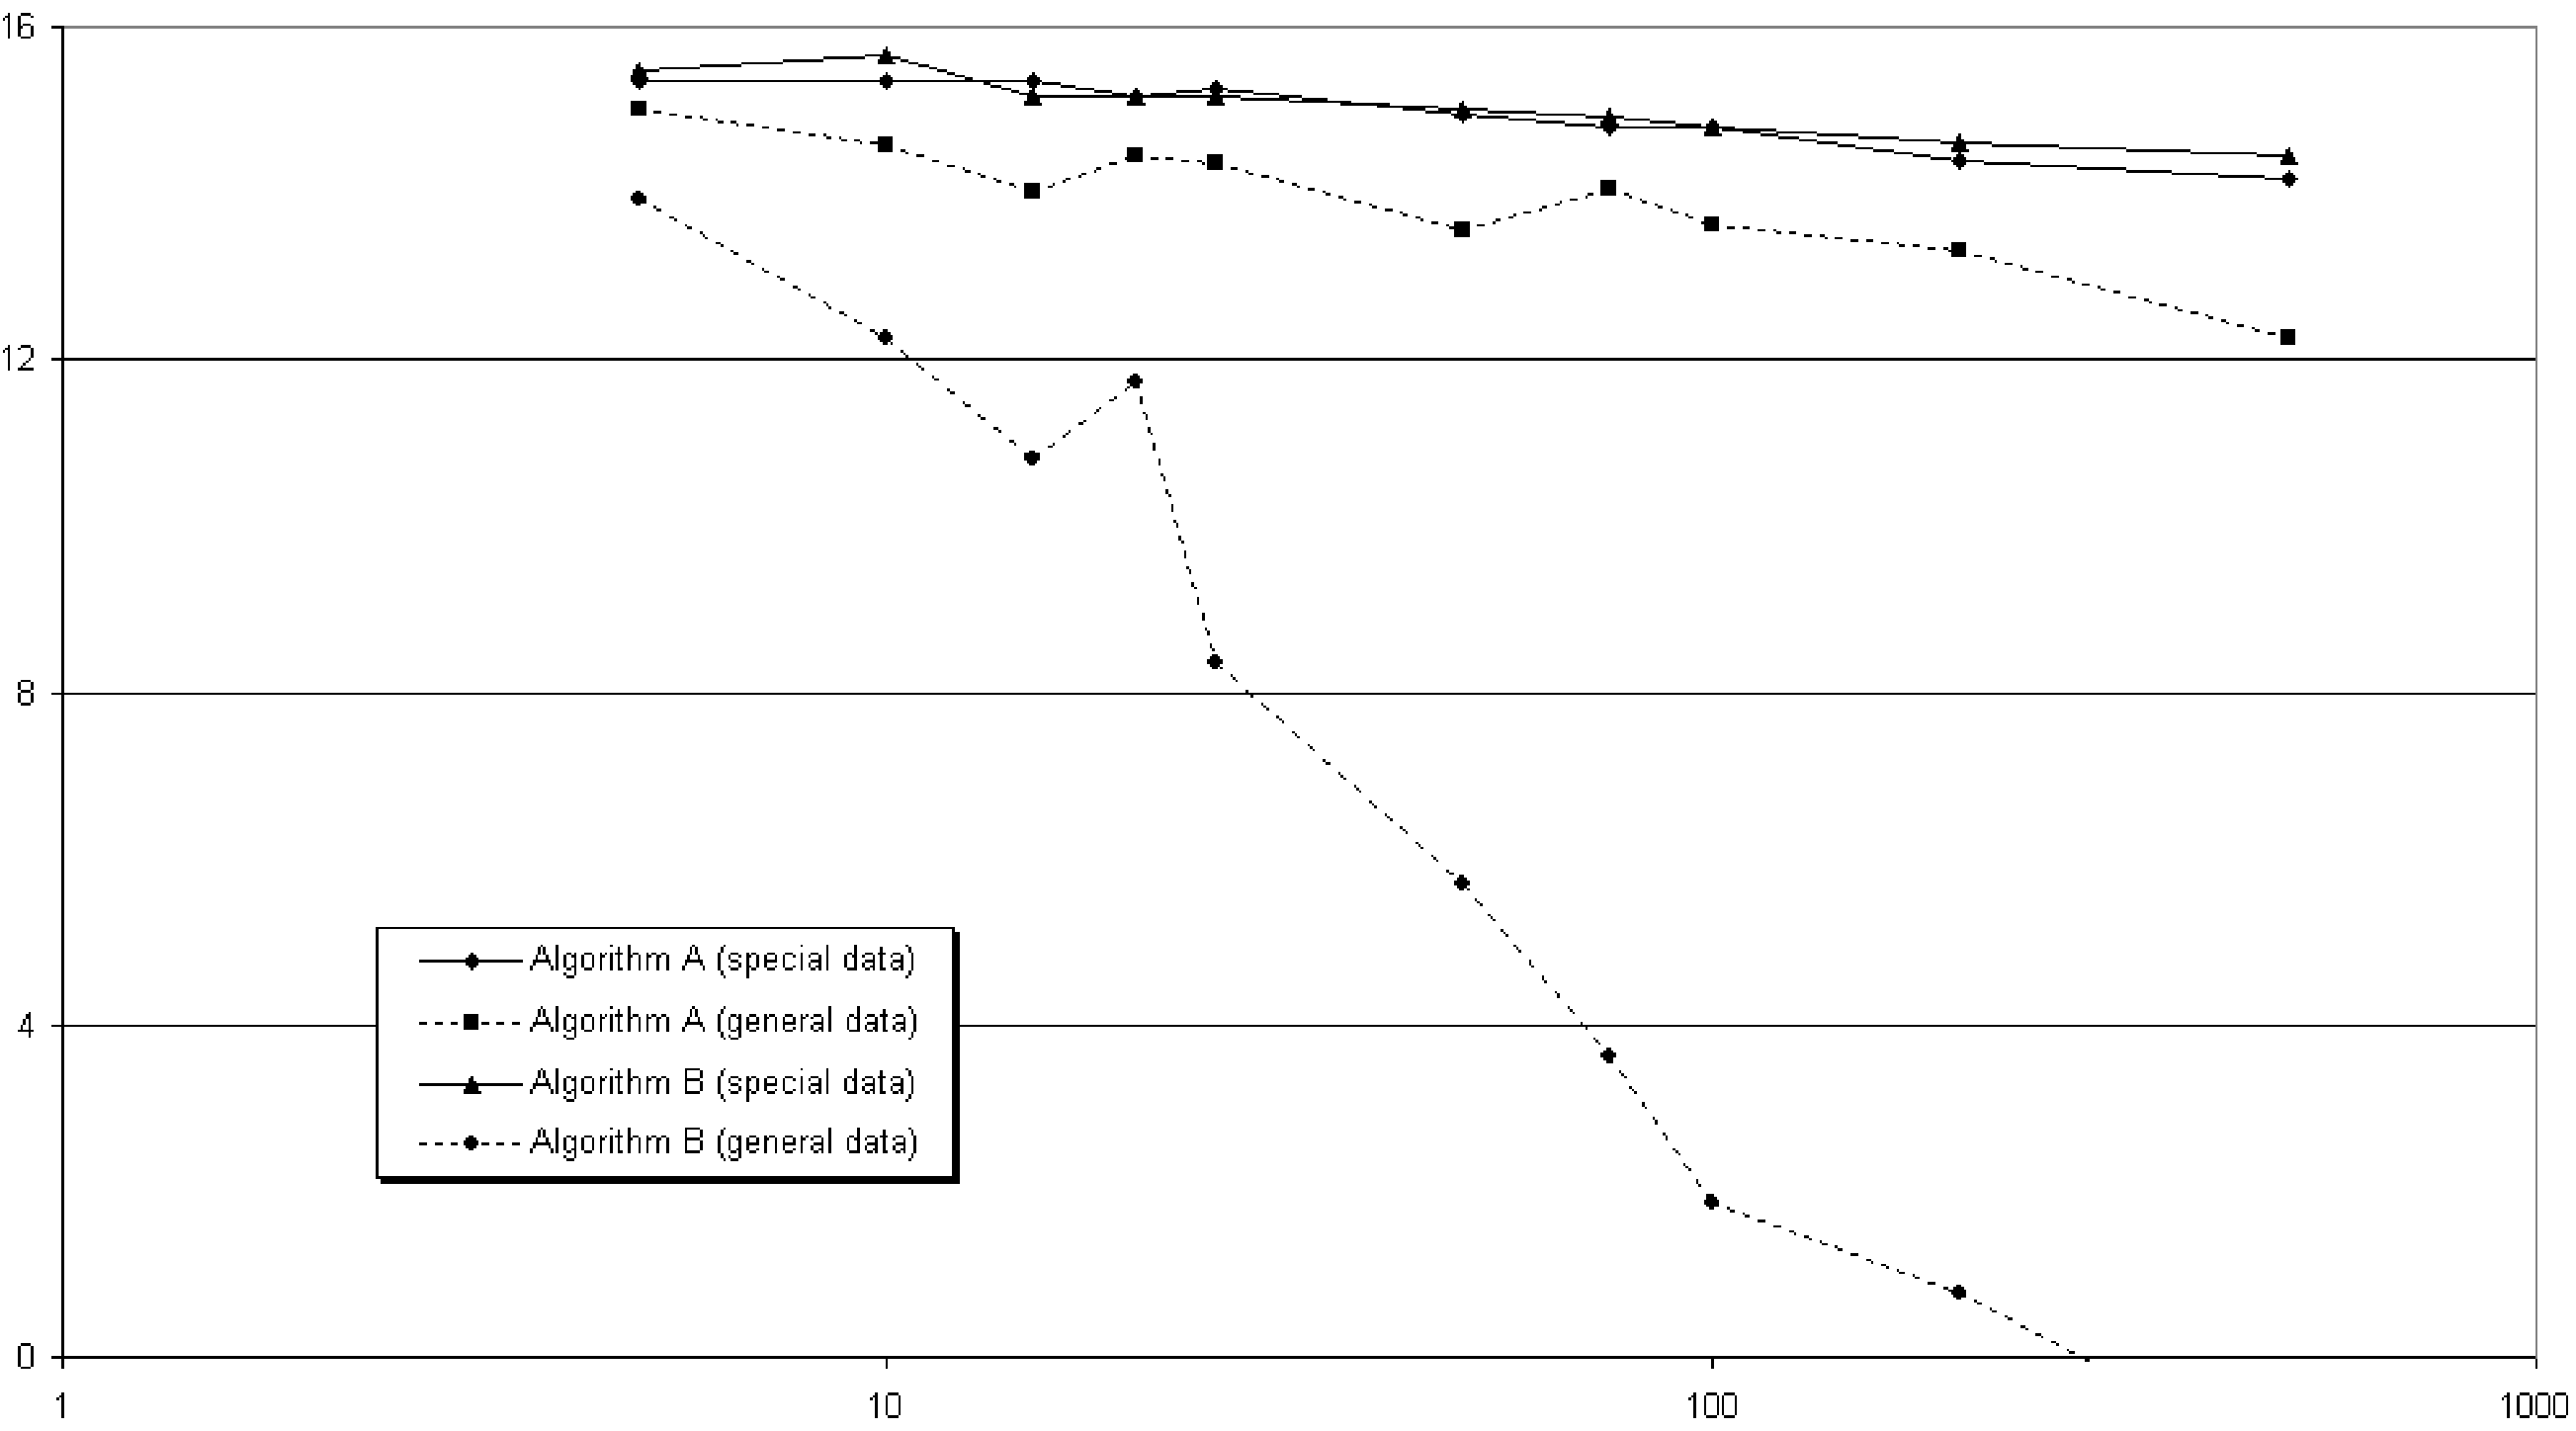
\includegraphics[width=12cm]{Figures/Precision}
\caption{Comparison of achieved precision} \label{fig:precision}
\end{figure}
Figure \ref{fig:precision} shows the results. The parameter
measuring the complexity is laid on the $x$-axis using a
logarithmic scale. The precision is expressed as the negative of
the decimal logarithm of the deviation from the known solution.
The higher the value the better is the precision. The precision of
the floating-point numbers on the machine used in this study
corresponds roughly to 16 on the scale of Figure
\ref{fig:precision}.

The first observation does not come as a surprise: the precision
of each algorithm degrades as the complexity of the problem
increases. One can see that when the algorithms can exploit the
symmetry properties of the data the precision is better (curves
for special data) than for general data. In this case the two
algorithms are performing with essentially the same precision.
Thus, one can chose the faster algorithm, namely algorithm B. For
the general data, however, algorithm B has poorer and poorer
precision as the complexity increases. For complexity larger than
50 algorithm B becomes totally unreliable, to the point of
becoming a perfect illustration of Knuth's quotation above. Thus,
for general data, one has no choice but to use algorithm A.

Readers who do not like mysteries can go read section
\ref{sec:matrixrounding} where these algorithms are discussed.

\subsection{Outsmarting rounding errors}
\label{sec:outsmart} In some instances rounding errors can be
significantly reduced if one spends some time reconsidering how to
compute the final solution. In this section we like to show an
example of such thinking.

Consider the following second order equation, which must be solved
when looking for the eigenvalues of a symmetric matrix (\cf
section \ref{sec:eigensym}):
\begin{equation}
\label{eq:round2nd}
  t^2+2\alpha t - 1 =0.
\end{equation}
Without restricting the generality of the argumentation, we shall
assume that $\alpha$ is positive. the problem is to find the the
root of equation \ref{eq:round2nd} having the smallest absolute
value. You, reader, should have the answer somewhere in one corner
of your brain, left over from high school mathematics:
\begin{equation}
\label{eq:round2ndsol}
  t_{\min}=\sqrt{\alpha^2+1} - \alpha.
\end{equation}
Let us now assume that $\alpha$ is very large, so large that
adding $1$ to $\alpha^2$ cannot be noticed within the machine
precision. Then, the smallest of the solutions of equation
\ref{eq:round2nd} becomes $t_{\min}\approx 0$, which is of course
not true: the left hand side of equation  \ref{eq:round2nd}
evaluates to $-1$.

\noindent Let us now rewrite equation \ref{eq:round2nd} for the
variable $x=1/t$. This gives the following equation:
\begin{equation}
\label{eq:round2ndinv}
  x^2-2\alpha x - 1 =0.
\end{equation}
The smallest of the two solutions of equation \ref{eq:round2nd} is
the largest of the two solutions of equation \ref{eq:round2ndinv}.
That is:
\begin{equation}
  t_{\min}={1\over x_{\max}}={1 \over \sqrt{\alpha^2+1} + \alpha}.
\end{equation}
Now we have for large $\alpha$:
\begin{equation}
  t_{\min}\approx {1\over 2\alpha}.
\end{equation}
This solution has certainly some rounding errors, but much less
than the solution of equation \ref{eq:round2ndsol}: the left hand
side of equation \ref{eq:round2nd} evaluates to ${1\over
4\alpha^2}$, which goes toward zero for large $\alpha$, as it
should be.

\subsection{Wisdom from the past}
To close the subject of rounding errors, I would like to give the
reader a different perspective. There is a big difference between
a full control of rounding errors and giving a result with high
precision. Granted, high precision computation is required to
minimize rounding errors. On the other hand, one only needs to
keep the rounding errors under control to a level up to the
precision required for the final results. There is no need to
determine a result with non-sensical precision.

To illustrate the point, I am going to use a very old mathematical
problem: the determination of the number $\pi$. The story is taken
from the excellent book of Jan Gullberg, {\em Mathematics From the
Birth of the Numbers} \cite{Gullberg}.

Around 300BC, Archimedes devised a simple algorithm to approximate
$\pi$. For a circle of diameter $d$, one computes the perimeter
$p_{\mathop{\textrm in}}$ of a $n$-sided regular polygon inscribed
within the circle and the perimeter $p_{\mathop{\textrm out}}$ of a
$n$-sided regular polygon whose sides the tangent to the same
circle. We have:
\begin{equation}
{\displaystyle p_{\mathop{\textrm in}} \over\displaystyle d
}<\pi<{\displaystyle p_{\mathop{\textrm out}} \over\displaystyle d}.
\end{equation}
By increasing $n$, one can improve the precision of the
determination of $\pi$. During the Antiquity and the Middle Age,
the computation of the perimeters was a formidable task and an
informal competition took place to find who could find the most
precise approximation of the number $\pi$. In 1424, Jamshid Masud
al-Kashi, a persian scientist, published an approximation of $\pi$
with 16 decimal digits. The number of sides of the polygons was
$3\times 2^8$. This was quite an achievement, the last of its
kind. After that, mathematicians discovered other means of
expressing the number $\pi$.

In my eyes, however, Jamshid Masud al-Kashi deserves fame and
admiration for the note added to his publication that places his
result in perspective. He noted that the precision of his
determination of the number $\pi$ was such that,
\begin{quote}{\textit the error
in computing the perimeter of a circle with a radius 600000 times
that of earth would be less than the thickness of a horse's hair}.
\end{quote}
The reader should know that the {\textit thickness of a horse's
hair\/} was a legal unit of measure in ancient Persia
corresponding to roughly 0.7 mm. Using present-day knowledge of
astronomy, the radius of the circle corresponding to the error
quoted by Jamshid Masud al-Kashi is 147 times the distance between
the sun and the earth, or about 3 times the radius of the orbit of
Pluto, the most distant planet of the solar system.

As Jan Gullberg notes in his book, {\textit al-Kashi evidently had a
good understanding of the meaninglessness of long chains of
decimals}. When dealing with numerical precision, you should ask
yourself the following question:
\begin{quote}
{\textsl Do I really need to know the length of Pluto's orbit to a
third of the thickness of a horse's hair?}
\end{quote}

\section{Finding the numerical precision of a computer}
\label{sec:findprecision}
Object-oriented languages such as Smalltalk give the
opportunity to develop an application on one hardware platform and
to deploy the application on other platforms running on different
operating systems and hardware.
It is a well-known fact that the
marketing about Java was centered about the concept of {\textsl Write
Once Run Anywhere}.
What fewer people know is that this concept
already existed for Smalltalk 10 years before the advent of Java.

Some numerical algorithms are carried until the estimated
precision of the result becomes smaller than a given value, called
the desired precision. Since an application can be executing on
different hardware, the desired precision is best determined at
run time.

The book of Press {\textit et al.} \cite{Press} shows a clever code
determining all the parameters of the floating-point
representation of a particular computer. In this book we shall
concentrate only on the parameters which are relevant for
numerical computations. These parameters correspond to the
instance variables of the object responsible to compute them. They
are the following:
\begin{description}
\item[\code{radix}] the radix of the floating-point representation, that is $r$.
\item[\code{machinePrecision}] the largest positive number which, when added to 1 yields 1.
\item[\code{negativeMachinePrecision}] the largest positive number which, when subtracted from 1 yields 1.
\item[\code{smallestNumber}] the smallest positive number different from 0.
\item[\code{largestNumber}] the largest positive number which can be represented in the machine.
\item[\code{defaultNumericalPrecision}] the relative precision, which can be expected for a general numerical computation.
\item[\code{smallNumber}] a number, which can be added to some value without noticeably changing the result of the computation.
\end{description}
Computing the radix $r$ is done in two steps. First one computes a
number equivalent of the machine precision (\cf next paragraph)
assuming the radix is 2. Then, one keeps adding 1 to this number
until the result changes. The number of added ones is the radix.

The machine precision is computed by finding the largest integer
$n$ such that:
\begin{equation}
\left(1+r^{-n}\right)-1\ne 0
\end{equation}
This is done with a loop over $n$. The quantity
$\epsilon_+=r^{-\left(n+1\right)}$ is the machine precision.

The negative machine precision is computed by finding the largest
integer $n$ such that:
\begin{equation}
\left(1-r^{-n}\right)-1\ne 0
\end{equation}
Computation is made as for the machine precision. The quantity
$\epsilon_-=r^{-\left(n+1\right)}$ is the negative machine
precision. If the floating-point representation uses
two-complement to represent negative numbers the machine precision
is larger than the negative machine precision.

To compute the smallest and largest number one first compute a
number whose mantissa is full. Such a number is obtained by
building the expression $f=1-r \times \epsilon_-$. The smallest
number is then computed by repeatedly dividing this value by the
radix until the result produces an underflow. The last value
obtained before an underflow occurs is the smallest number.
Similarly, the largest number is computed by repeatedly
multiplying the value $f$ until an overflow occurs. The last value
obtained before an overflow occurs is the largest number.

The variable \code{defaultNumericalPrecision} contains an estimate
of the precision expected for a general numerical computation. For
example, one should consider that two numbers $a$ and $b$ are
equal if the relative difference between them is less than the
default numerical machine precision. This value of the default
numerical machine precision has been defined as the square root of
the machine precision.

The variable \code{smallNumber} contains a value, which can be
added to some number without noticeably changing the result of the
computation. In general an expression of the type $0 \over 0$ is
undefined. In some particular case, however, one can define a
value based on a limit. For example, the expression $\sin x \over
x $ is equal to 1 for $x=0$. For algorithms, where such an
undefined expression can occur\footnote{Of course, after making
sure that the ratio is well defined numerically.}, adding a small
number to the numerator and the denominator can avoid the division
by zero exception and can obtain the correct value. This value of
the small number has been defined as the square root of the
smallest number that can be represented on the machine.

\subsection{Computer numerical precision}
The computation of the parameters only needs to be executed once.
We have introduced a specific class to hold the variables
described earlier and made them available to any object.

Each parameter is computed using lazy initialization within the
method bearing the same name as the parameter. Lazy initialization
is used while all parameters may not be needed at a given time.
Methods in charge of computing the parameters are all prefixed
with the word compute.

Listing below shows the class \code{PMFloatingPointMachine} responsible of computing the parameters
of the floating-point representation.
This class is implemented as a singleton class because the parameters need to be computed once
only. For that reason no code optimization was made and priority
is given to readability.

\begin{displaycode}{Smalltalk}
Object subclass: #PMFloatingPointMachine
  instanceVariableNames: 'defaultNumericalPrecision radix machinePrecision negativeMachinePrecision smallestNumber largestNumber smallNumber largestExponentArgument'
  classVariableNames: 'UniqueInstance'
  package: 'Math-Core'
\end{displaycode}

\begin{displaycode}{Smalltalk}
PMFloatingPointMachine class >> new
   UniqueInstance = nil
        ifTrue: [ UniqueInstance := super new].
   ^ UniqueInstance
\end{displaycode}

\begin{displaycode}{Smalltalk}
PMFloatingPointMachineMachine >> reset
   UniqueInstance := nil
\end{displaycode}

\noindent The computation of the smallest and largest numbers uses
exceptions to detect the underflow and the overflow.

\begin{displaycode}{Smalltalk}
PMFloatingPointMachine >> computeLargestNumber
    | zero one floatingRadix fullMantissaNumber |
    zero := 0 asFloat.
    one := 1 asFloat.
    floatingRadix := self radix asFloat.
    fullMantissaNumber := one - ( floatingRadix * self negativeMachinePrecision).
    largestNumber := fullMantissaNumber.
    [ [ fullMantissaNumber := fullMantissaNumber * floatingRadix.
        largestNumber := fullMantissaNumber.
        true] whileTrue: [ ].
        ] when: ExAll do: [ :signal | signal exitWith: nil].
\end{displaycode}

\begin{displaycode}{Smalltalk}
PMFloatingPointMachine >> computeMachinePrecision
    | one zero a b inverseRadix tmp x |
    one := 1 asFloat.
    zero := 0 asFloat.
    inverseRadix := one / self radix asFloat.
    machinePrecision := one.
    [ tmp := one + machinePrecision.
      tmp - one = zero]
        whileFalse:[  machinePrecision := machinePrecision * inverseRadix].
\end{displaycode}

\begin{displaycode}{Smalltalk}
PMFloatingPointMachine >> computeNegativeMachinePrecision
    | one zero floatingRadix inverseRadix tmp |
    one := 1 asFloat.
    zero := 0 asFloat.
    floatingRadix := self radix asFloat.
    inverseRadix := one / floatingRadix.
    negativeMachinePrecision := one.
    [ tmp := one - negativeMachinePrecision.
      tmp - one = zero]
        whileFalse: [ negativeMachinePrecision := 
                             negativeMachinePrecision * inverseRadix].
\end{displaycode}

\begin{displaycode}{Smalltalk}
PMFloatingPointMachine >>computeRadix
   | one zero a b tmp1 tmp2 |
   one := 1 asFloat.
   zero := 0 asFloat.
   a := one.
   [ a := a + a.
      tmp1 := a + one.
      tmp2 := tmp1 - a.
      tmp2 - one = zero] whileTrue: [].
    b := one.
    [ b := b + b.
      tmp1 := a + b.
      radix := ( tmp1 - a) truncated.
      radix = 0 ] whileTrue: [].
\end{displaycode}

\begin{displaycode}{Smalltalk}
PMFloatingPointMachine >> computeSmallestNumber
    | zero one floatingRadix inverseRadix fullMantissaNumber |
    zero := 0 asFloat.
    one := 1 asFloat.
    floatingRadix := self radix asFloat.
    inverseRadix := one / floatingRadix.
    fullMantissaNumber := one - ( floatingRadix * self negativeMachinePrecision).
    smallestNumber := fullMantissaNumber.
    [ [ fullMantissaNumber := fullMantissaNumber * inverseRadix.
        smallestNumber := fullMantissaNumber.
        true] whileTrue: [ ].
        ] when: ExAll do: [ :signal | signal exitWith: nil ].
\end{displaycode}

\begin{displaycode}{Smalltalk}
PMFloatingPointMachine >> defaultNumericalPrecision
    defaultNumericalPrecision isNil
        ifTrue: [ defaultNumericalPrecision := self machinePrecision sqrt ].
    ^defaultNumericalPrecision
\end{displaycode}

\begin{displaycode}{Smalltalk}
PMFloatingPointMachine >> largestExponentArgument
    largestExponentArgument isNil
        ifTrue: [ largestExponentArgument := self largestNumber ln].
    ^largestExponentArgument
\end{displaycode}

\begin{displaycode}{Smalltalk}
PMFloatingPointMachine >>largestNumber
    largestNumber isNil
        ifTrue: [ self computeLargestNumber ].
    ^largestNumber
\end{displaycode}

\begin{displaycode}{Smalltalk}
PMFloatingPointMachine >> machinePrecision
    machinePrecision isNil
        ifTrue: [ self computeMachinePrecision ].
    ^machinePrecision
\end{displaycode}

\begin{displaycode}{Smalltalk}
PMFloatingPointMachine >> negativeMachinePrecision
    negativeMachinePrecision isNil
        ifTrue: [ self computeNegativeMachinePrecision ].
    ^negativeMachinePrecision
\end{displaycode}

\begin{displaycode}{Smalltalk}
PMFloatingPointMachine >> radix
    radix isNil
        ifTrue: [ self computeRadix ].
    ^radix
\end{displaycode}

\noindent The method \code{showParameters} can be used to print the
values of the parameters onto the Transcript window.

\begin{displaycode}{Smalltalk}
PMFloatingPointMachine >> showParameters
  Transcript cr; cr;
    nextPutAll: 'Floating-point machine parameters'; cr;
    nextPutAll: '---------------------------------';cr;
    nextPutAll: 'Radix: '.
  self radix printOn: Transcript.
  Transcript cr; nextPutAll: 'Machine precision: '.
  self machinePrecision printOn: Transcript.
  Transcript cr; nextPutAll: 'Negative machine precision: '.
  self negativeMachinePrecision printOn: Transcript.
  Transcript cr; nextPutAll: 'Smallest number: '.
  self smallestNumber printOn: Transcript.
  Transcript cr; nextPutAll: 'Largest number: '.
  self largestNumber printOn: Transcript.
  Transcript flush
\end{displaycode}

\begin{displaycode}{Smalltalk}
PMFloatingPointMachine >> smallestNumber
    smallestNumber isNil
        ifTrue: [ self computeSmallestNumber ].
    ^smallestNumber
\end{displaycode}

\begin{displaycode}{Smalltalk}
PMFloatingPointMachine >> smallNumber
    smallNumber isNil
        ifTrue: [ smallNumber := self smallestNumber sqrt ].
    ^smallNumber
\end{displaycode}

\section{Comparing floating point numbers}
It is very surprising to see how frequently questions about the
lack of equality between two floating-point numbers are posted on
the Smalltalk electronic discussion groups. As we have
seen in section \ref{sec-rounding} one should always expect the
result of two different computations that should have yielded the
same number from a mathematical standpoint to be different using a
finite  numerical representation. Somehow the computer courses are
not giving enough emphasis about floating-point numbers.

\begin{quote}
So, how should you check the equality of two floating-point
numbers? The practical answer is: {\textsl thou shalt not!}
\end{quote}

\noindent As you will see, the algorithms in this book only
compare numbers, but never check for equality. If you cannot
escape the need for a test of equality, however, the best solution
is to create methods to do this. Since the floating-point
representation is keeping a constant relative precision,
comparison must be made using relative error. Let $a$ and $b$ be
the two numbers to be compared. One should build the following
expression:
\begin{equation}
\label{eq:relerror}
\epsilon={\left|a-b\right| \over
\max\left(\left|a\right|,\left|b\right|\right)}
\end{equation}
The two numbers can be considered equal if $\epsilon$ is smaller
than a given number $\epsilon_{\max}$. If the denominator of the
fraction on equation \ref{eq:relerror} is less than
$\epsilon_{\max}$, than the two numbers can be considered as being
equal. For lack of information on how the numbers $a$ and $b$ have
been obtained, one uses for $\epsilon_{\max}$ the default
numerical precision defined in section \ref{sec:findprecision}.
If one can determine the precision of each number, then the method \code{relativelyEqual} can be used.

In Smalltalk this means adding a new method to the class Number as
shown in Listing \ref{lst:fltcompare}.

\begin{listing}[label=lst:fltcompare]{Smalltalk}
{Comparison of floating point numbers in Smalltalk}
Number >> equalsTo: aNumber
   ^self relativelyEqualsTo: aNumber upTo:
         PMFloatingPointMachine new defaultNumericalPrecision
\end{listing}

\begin{displaycode}{Smalltalk}
Number >> relativelyEqualsTo: aNumber upTo: aSmallNumber
   | norm |
   norm := self abs max: aNumber abs.
   ^norm <= PMFloatingPointMachine new defaultNumericalPrecision
    or: [ (self - aNumber) abs < ( aSmallNumber * norm)]
\end{displaycode}

\section{Speed consideration (to be revisited)}
\label{sec:speed} Some people may think that implementing
numerical methods for object-oriented languages such as Smalltalk just a waste
of time. Those languages are notoriously slow or so they think.

First of all, things should be put in perspective with other
actions performed by the computer. If a computation does not take
longer than the time needed to refresh a screen, it does not
really matter if the application is interactive. For example,
performing a least square fit to a histogram in Smalltalk and drawing the
resulting fitted function is usually hardly perceptible to the eye on a personal
computer. Thus, even though a C version runs 10 times faster, it
does not make any difference for the end user. The main difference
comes, however, when you need to modify the code. Object-oriented
software is well known for its maintainability. As $80\%$ of the
code development is spent in maintenance this aspect should first
be considered.

Table \ref{tb:speed} shows measured speed of execution for some of
the algorithms exposed in this book. Timing was done on a personal
computer equipped with a Pentium II clocked at 200MHz and running
Windows NT workstation 4.0. The C code used is the code of
\cite{Press} compiled with the C compiler Visual C$^{++}$ 4.0 from
Microsoft Corporation. The time needed to allocate memory for
intermediate results was included in the measurement of the C
code, otherwise the comparison with object-oriented code would not
be fair. The Smalltalk code was run under version 4.0 of Visual
Age\tm for Smalltalk from IBM Corporation using the ENVY benchmark
tool provided.
Elapsed time were measured
by repeating the measured evaluation a sufficient number of time
so that the error caused by the CPU clock is less that the last
digit shown in the final result.
\begin{table}[h]
\caption{Compared execution speed between C and Smalltalk}
\label{tb:speed} \vspace{1 ex}
\begin{tabular}{|l | c r r |} \hline
  \hfil {\textbf Operation} & {\textbf Units} & {\textbf C}\hfil & {\textbf Smalltalk}\hfil \\ \hline
  Polynomial $10\th$ degree & msec. & 1.1 & 27.7 \\
  Neville interpolation (20 points) & msec. & 0.9 & 11.0 \\
  LUP matrix inversion ($100\times 100$)& sec. & 3.9 & 22.9 \\ \hline
\end{tabular}
\end{table}

One can see that object-oriented code is quite efficient,
especially when it comes to complex algorithms: good
object-oriented code can actually beat up C code.

%My early tests with Java, a couple of years ago, were showing that
%Java was 5-10 times slower than C. One can see that vendors did a
%great job in optimizing the generated code and in accelerating the
%virtual machine. I would like to see the same efforts going in
%optimizing Smalltalk. The spectacular improvement of Java shows
%that it is possible. Actually, my early tests made with Visual
%Smalltalk\tm from Digitalk Inc.\footnote{Unfortunately, the future
%of Visual Smalltalk now owned by Cincom Inc. is quite uncertain at
%this time of writing.} were 5 times better.

%Today admittedly, I would not use Smalltalk to build a structural
%analysis program, but Java would certainly be a contender.
I have successfully build data mining Smalltalk
applications using {\textbf all the code}\footnote{I want to emphasize
here that all the code of this book is real code, which I have
used personally in real applications.} presented in this book.
These applications were not perceived as slow by the end user
since most of the computer time was spent drawing the data.

\subsection{Smalltalk particular}
Smalltalk has an interesting property: a division between two
integers is by default kept as a fraction. This prevents rounding
errors. For example, the multiplication of a matrix of integer
numbers with its inverse always yields an exact identity matrix.
(\cf section \ref{sec:lup} for definitions of these terms).

There is, however, a price to pay for the perfection offered by
fractions. When using fractions, the computing time often becomes
prohibitive. Resulting fractions are often composed of large
integers. This slows down the computing. In the case of matrix
inversion, this results in an increase in computing time by
several orders of magnitude.

For example, one of my customers was inverting a $301\times 301$
matrix with the code of section \ref{sec:lup}. The numbers used to
build the matrix where obtained from a measuring device (using an
ADC) and where thus integers. The inversion time was over 2
hours\footnote{This particular customer was a {\textsl very} patient
person!}. After converting the matrix components to floating
numbers the inversion time became less than 30 seconds!

If you are especially unlucky you may run out of memory when
attempting to store a particularly long integer. Thus, it is
always a good idea to use floating\footnote{In most available
Smalltalk versions the class Float corresponds to floating numbers
with double precision. VisualWorks makes the difference between
\code{Float} and \code{Double}} numbers instead of fractions unless
absolute accuracy is your primary goal. My experience has been
that using floating numbers speeds up the computation by at least
an order of magnitude.
In the case of complex computations such as
matrix inversion or least square fit this can become prohibitive.

\section{Conventions}
Equations presented in this book are using standard international
mathematical notation as described in \cite{Knuth1}. Each section
is trying to made a quick derivation of the concepts needed to
fully understand the mathematics behind the scene. For readers in
a hurry, the equations used by the implementation are flagged as
the following sample equation:
\begin{mainEquation}
\ln ab = \ln a + \ln b.
\end{mainEquation}
When such an equation is encountered, the reader is sure that the
expression is implemented in the code.

In general the code presented in this book adheres to conventions
widely used in each language. Having said that, there are a few
instances where we have departed from the widely used conventions.

\subsection{Class diagrams}
When appropriate a class diagram is shown at the beginning of each
chapter. This diagram shows the hierarchy of the classes described
in the chapter and eventually the relations with classes of other
chapters. The diagrams are drawn using the conventions of the book
on design patterns \cite{GoF}.

Figure \ref{fig:classDiagram} shows a typical class diagram. A
rectangular box with 2 or 3 parts represents a class. The top part
contains the name of the class in bold face. If the class is an
abstract class the name in shown in italic bold face.
In figure \ref{fig:classDiagram} the classes \code{RelatedClass}, \code{MySubClass1} and \code{MySubclass2} are concrete classes; \code{MyAbstractClass} is an abstract class.
The second part of the class box contains a list of the public instance methods.
The name of an abstract method is written in italic, for example \code{abstractMethod3} in the class \code{MyAbstractClass} of figure \ref{fig:classDiagram}.
The third part of the class box, if any, contains the list of all instance variables.
If the class does not
have any instance variable the class box only consists of 2 parts,
for example the class \code{MySubClass1} of figure
\ref{fig:classDiagram}.
\begin{figure}
\centering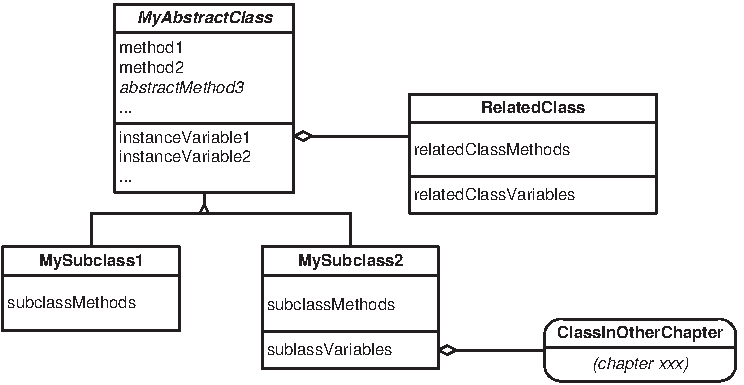
\includegraphics[width=11cm]{Figures/TypicalClassDiagram}
\caption{A typical class diagram} \label{fig:classDiagram}
\end{figure}

A vertical line with a triangle indicates class inheritance. If
there are several subclasses the line branches at the triangle, as
this is the case in figure \ref{fig:classDiagram}. A horizontal
line beginning with a diamond (UML aggregation symbol) indicates
the class of an instance variable. For example, Figure
\ref{fig:classDiagram} indicates that the instance variable \code{instanceVariable1} of the class \code{MyAbstractClass} must be an
instance of the class \code{RelatedClass}. The diamond is black is
the instance variable is a collection of instances of the class. A
class within a rectangle with rounded corner represents a class
already discussed in an earlier chapter; the reference to the
chapter is written below the class name. Class \code{ClassInOtherChapter} in figure \ref{fig:classDiagram} is such a
class. To save space, we have used the
Smalltalk method names. It is quite easy to identify methods
needing parameters when one uses Smalltalk method names: a
colon in the middle or at the end of the method name indicates
a parameter. Please refer to appendix \ref{ch:smalltalkprimer} for
more details on Smalltalk methods.

\subsection{Smalltalk code}
Most of the Smalltalk systems do not support name spaces. As a
consequence, it has becomed a convention to prefix all class names
with 3-letter code identifying the origin of the code. In this
book the names of the Smalltalk classes are all prefixed with PM like PolyMath\footnote{Classes were previously prefixed with author's initials.}.

There are several ways to store constants needed by all instances
of a class. One way is to store the constants in class variables.
This requires each class to implement an initialization method,
which sets the desired values into the class variables. Another
way is to store the constants in a pool dictionary. Here also an
initialization method is required. In my opinion pool dictionaries
are best used for texts, as they provide a convenient way to
change all text from one language to another. Sometimes the
creation of a singleton object is used. This is especially useful
when the constants are installation specific and, therefore, must
be determined at the beginning of the application's execution,
such as the precision of the machine (\cf section
\ref{sec:findprecision}). Finally constants which are not likely
to change can be stored in the code. This is acceptable as long as
this is done at a unique place. In this book most constants are
defined in class methods.

By default a Smalltalk method returns \code{self}. For
initialization methods, however, we write this return explicitly
(\code{^self}) to ease reading. This adheres to the intention
revealing patterns of Kent Beck \cite{Beck}.

In \cite{StDesPat} it is recommended to use the method name \code{default} to implement a singleton class. In this book this
convention is not followed. In Smalltalk, however, the normal
instance creation method is \code{new}. Introducing a method \code{default} for singleton classes has the effect of departing from
this more ancient convention. In fact, requiring the use of \code{default} amounts to reveal to the client the details of
implementation used by the class. This is in clear contradiction
with the principle of hiding the implementation to the external
world.
Thus, singleton classes in all code presented in this book
are obtained by sending the method \code{new} to the class.
A method named \code{default} is reserved for the very semantic of
the word default: the instance returned by these methods is an
instance initialized with some default contents, well specified.
Whether or not the instance is a singleton is not the problem of
the client application.

\section{Roadmap}
This last section of the introduction describes the roadmap of
the algorithms discussed in the book chapter by chapter. Figure
\ref{fig:roadmap} shows a schematic view of the major classes
discussed in this book together with their dependency relations.
\begin{figure}
\centering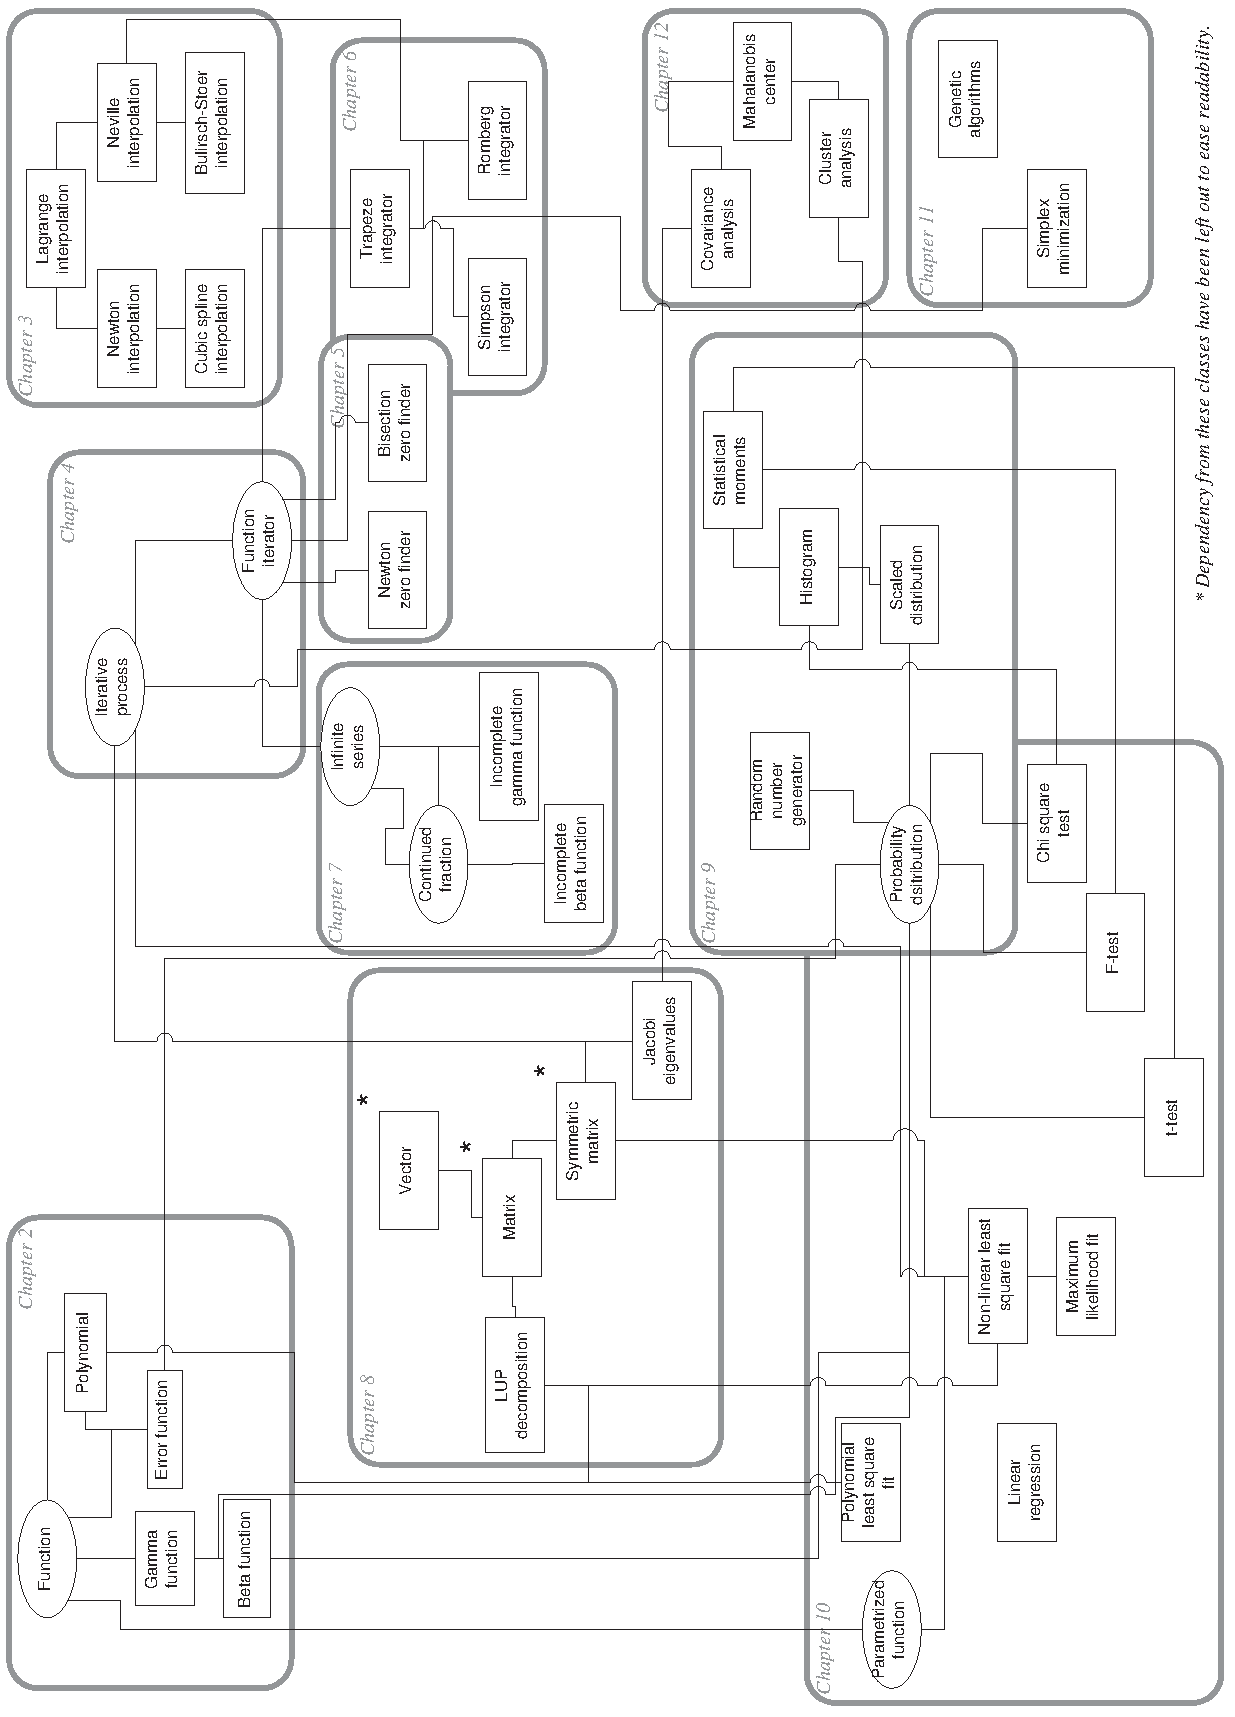
\includegraphics[width=13cm]{Figures/Roadmap}
\caption{Book roadmap} \label{fig:roadmap}
\end{figure}
In this figure, abstract classes are represented with an ellipse,
concrete classes with a rectangle. Dependencies between the
classes are represented by lines going from one class to another;
the dependent class is always located below. Chapters where the
classes are discussed are drawn as grayed rectangles with rounded
corners. Hopefully the reader will not be scared by the complexity
of the figure. Actually, the figure should be more complex as the
classes \code{Vector} and \code{Matrix} are used by most objects
located in chapters \ref{ch:linearalgebra} and following. To
preserve the readability of figure \ref{fig:roadmap} the
dependency connections for these two classes have been left out.

Chapter \ref{ch:function} presents a general representation of
mathematical functions. Examples are shown. A concrete
implementation of polynomial is discussed. Finally three library
functions are given: the error function, the gamma function and
the beta function.

Chapter \ref{ch:interpolation} discusses interpolation algorithms.
A discussion explains when interpolation should be used and which
algorithm is more appropriate to which data.

Chapter \ref{ch:iteration} presents a general framework for
iterative process. It also discusses a specialization of the
framework to iterative process with a single numerical result.
This framework is widely used in the rest of the book.

Chapter \ref{ch:zeroes} discusses two algorithms to find the
zeroes of a function: bisection and Newton's zero finding
algorithms. Both algorithms use the general framework of chapter
\ref{ch:iteration}.

Chapter \ref{ch:integration} discusses several algorithms to
compute the integral of a function. All algorithms are based on
the general framework of chapter \ref{ch:iteration}. This chapter
also uses an interpolation technique from chapter
\ref{ch:interpolation}.

Chapter \ref{ch:series} discusses the specialization of the
general framework of chapter \ref{ch:iteration} to the computation
of infinite series and continued fractions. The incomplete gamma
function and incomplete beta function are used as concrete
examples to illustrate the technique.

Chapter \ref{ch:linearalgebra} presents a concrete implementation
of vector and matrix algebra. It also discusses algorithms to
solve systems of linear equations. Algorithms to compute matrix
inversion and the finding of eigenvalues and eigenvectors are
exposed. Elements of this chapter are used in other part of this
book.

Chapter \ref{ch:statistics} presents tools to perform statistical
analysis. Random number generators are discussed. We give an
abstract implementation of a probability distribution with
concrete example of the most important distributions. The
implementation of other distributions is given in appendix. This
chapter uses techniques from chapters \ref{ch:function},
\ref{ch:zeroes} and \ref{ch:integration}.

Chapter \ref{ch:estimation} discussed the test of hypothesis and
estimation. It gives an implementation of the t- and F-tests. It
presents a general framework to implement least square fit and
maximum likelihood estimation. Concrete implementations of least
square fit for linear and polynomial dependence are given. A
concrete implementation of the maximum likelihood estimation is
given to fit a probability distribution to a histogram. This
chapter uses techniques from chapter \ref{ch:function},
\ref{ch:iteration}, \ref{ch:linearalgebra} and
\ref{ch:statistics}.

Chapter \ref{ch:minimization} discusses some techniques used to
maximize or minimize a function: classical algorithms (simplex,
hill climbing) as well as new ones (genetic algorithms). All these
algorithms are using the general framework for iterative process
discussed in chapter \ref{ch:iteration}.

Chapter \ref{ch:datamining} discusses the modern data mining
techniques: correlation analysis, cluster analysis and neural
networks. A couple of methods invented by the author are also
discussed. This chapter uses directly or indirectly techniques
from all chapters of this book.

%\ifx\wholebook\relax\else\end{document}\fi

%\ifx\wholebook\relax\else
%\documentclass[twoside]{book}
%\usepackage[active]{srcltx}
%\usepackage[LY1]{fontenc}
%\usepackage{url}
\makeatletter
\def\url@leostyle{%
  \@ifundefined{selectfont}{\def\UrlFont{\sf}}{\def\UrlFont{\sffamily}}}
\makeatother
% Now actually use the newly defined style.
\urlstyle{leo}

\usepackage{graphicx}
\def\etc{{\textit{etc}}}
\def\eg{{\textit{e.g.}}}
\def\ie{{\textit{i.e.}}}
\def\cf{{\textit{c.f.}}\ }
\def\erf{\mathop{\textrm{erf}}}
\def\sign{\mathop{\textrm{sign}}}
\def\prob{\mathop{\textrm{Prob}}}
\def\var{\mathop{\textrm{var}}}
\def\mod{\mathop{\textrm{mod}}}
\def\cor{\mathop{\textrm{cor}}}
\def\cov{\mathop{\textrm{cov}}}
\def\cl{\mathop{\textrm{CL}}}
\def\kg{\mathop{\textrm{Kg}}}
\def\patstyle#1{{\textsc #1}}
\def\th{^{\mathop{\textrm{th}}}}
%\def\st#1{^{\mathop{\rm #1}}}
\def\note#1{\begin{quote}{\textbf{Note:}} #1\end{quote}}
\def\braket#1{\left\langle #1\right\rangle}
\def\order#1{\let\o=#1$\mathcal{O}$\ifx\o 1$\left(n\right)$\else$\left(n^{#1}\right)$\fi}
%\newtheorem{privListing}{Listing}[chapter]
%\newenvironment{listing}{\vskip 3ex\hrule\vskip 1ex\begin{privListing}}{\end{privListing}\hrule\vskip 1ex}
\newtheorem{privExample}{Code example}[chapter]
\newenvironment{codeExample}{\begin{privExample}\begin{quote}\tt}{\end{quote}\end{privExample}}
\def\relboxl#1#2{\hbox to #1\hsize{#2\hfil}}
\def\relboxc#1#2{\hbox to #1\hsize{\hfil #2\hfil}}
\def\relboxr#1#2{\hbox to #1\hsize{\hfil #2}}
\def\transpose#1{\textbf{#1}^{\mathop\textrm{T}}}
\def\inverse#1{\textbf{#1}^{-1}}
%\def\tm{$^{\mathop{\rm TM}}$}
\def\tm{ }
\newenvironment{mainEquation}{\marginpar[\vspace{3 ex} Main
equation$\Rightarrow$]{\vspace{3 ex}$\Leftarrow$Main
equation}\begin{equation}}{\end{equation}}
\def\rubrique#1{\paragraph{#1}\hfil\par\noindent}

%\begin{document}
%\fi

\chapter{Function evaluation}
\label{ch:function} \vspace{1 ex}
\begin{flushright}
{\textsl Qu'il n'y ait pas de r\'eponse n'excuse pas l'absence de
questions.}\footnote{The absence of answer does not justify the
absence of question.}\\ Claude Roy
\end{flushright}
\vspace{1 ex} Many mathematical functions used in numerical
computation are defined by an integral, by a recurrence formula or
by a series expansion. While such definitions can be useful to a
mathematician, they are usually quite complicated to implement on
a computer. For one, not every programmer knows how to evaluate an
integral numerically\footnote{The good news is that they will if
they read the present book (\cf chapter \ref{ch:integration}).}.
Then, there is the problem of accuracy. Finally, the evaluation of
the function as defined mathematically is often too slow to be
practical.

Before computers were heavily used, however, people had already
found efficient ways of evaluating complicated functions. These
methods are usually precise enough and extremely fast. This
chapter exposes several functions that are important for
statistical analysis. The Handbook of Mathematical Functions by
Abramovitz and Stegun \cite{AbrSteg} contains a wealth of such
function definitions and describes many ways of evaluating them
numerically. Most approximations used in this chapter have been
taken from this book.

This chapter opens on general considerations on how to implement
the concept of function. Then, polynomials are discussed as an
example of concrete function implementation. The rest of this
chapter introduces three classical functions: the error function,
the gamma function and the beta function. We shall use this
functions in chapters \ref{ch:statistics} and \ref{ch:estimation}.
Because these functions are fundamental functions used in many
areas of mathematics they are implemented as library functions ---
such as a sine, log or exponential --- instead of using the
general function formalism described in the first section.

Figure \ref{fig:functions} shows the diagram of the Smalltalk classes
described in this chapter.
\begin{figure}
\centering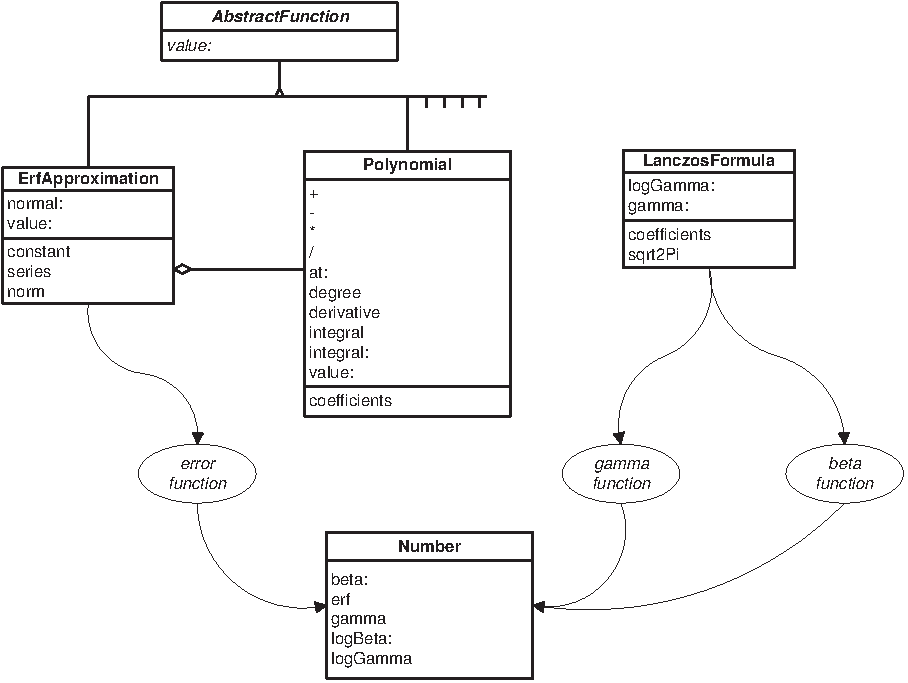
\includegraphics[width=10cm]{Figures/FunctionS}
\caption{Smalltalk classes related to functions}
\label{fig:functions}
\end{figure}
Here we have used special notations to indicate that the functions
are implemented as library functions. The functions are
represented by oval and arrows shows which class is used to
implement a function for the class \code{Number}.

\section{Function concept}
\label{sec:function}
A mathematical function is an object
associating a value to a variable. If the variable is a single
value one talks about a one variable function. If the variable is
an array of values one talks about a multi-variable function.
Other types of variables are possible but will not be covered in
this book.

We shall assume that the reader is familiar with elementary
concepts about functions, namely derivatives and integrals. We
shall concentrate mostly on implementation issues.

\section{Function -- Smalltalk implementation}
\label{sec:stFunction}
A mathematical function is an object
associating a value to a variable. If the variable is a single
value one talks about a one variable function. If the variable is
an array of values one talks about a multi-variable function.
Other types of variables are possible but will not be covered in
this book.

We shall assume that the reader is familiar with elementary
concepts about functions, namely derivatives and integrals. We
shall concentrate mostly on implementation issues.

\marginpar{Figure \ref{fig:functions} with
the box \code{AbstractFunction} grayed.} A function in Smalltalk
can be readily implemented with a block closure. Block closures in
Smalltalk are treated like objects; thus, they can be manipulated
as any other objects. For example the one variable function
defined as:
\begin{equation}
f\left( x \right)={1 \over x},
\end{equation}
can be implemented in Smalltalk as:
\begin{displaycode}{Smalltalk}
f := [:x | 1 / x].
\end{displaycode}
Evaluation of a block closure is supplied by the method value:.
For example, to compute the inverse of 3, one writes:
\begin{displaycode}{Smalltalk}
f value: 3.
\end{displaycode}

If the function is more complex a block closure may not be the
best solution to implement a function. Instead a class can be
created with some instance variables to hold any constants and/or
partial results. In order to be able to use functions
indifferently implemented as block closures or as classes, one
uses polymorphism. Each class implementing a function must
implement a method \code{value:}.
Thus, any object evaluating a function can send the same message selector, namely \code{value:}, to the variable
holding the function.

To evaluate a multi-variable function, the argument of the method
\code{value:} is an Array or a vector (\cf section
\ref{sec:linearalgebra}). Thus, in Smalltalk multi-variable
functions can follow the same polymorphism as for one-variable
functions.

\section{Polynomials}
\label{sec:polynomial}
 Polynomials are quite important in
numerical methods because they are often used in approximating
functions. For example, section \ref{sec:errorFunction} shows how
the error function can be approximated with the product of normal
distribution times a polynomial.

Polynomials are also useful in approximating functions, which are
determined by experimental measurements in the absence of any
theory on the nature of the function. For example, the output of a
sensor detecting a coin is dependent on the temperature of the
coin mechanism. This temperature dependence cannot be predicted
theoretically because it is a difficult problem. Instead, one can
measure the sensor output at various controlled temperatures.
These measurements are used to determine the coefficients of a
polynomial reproducing the measured temperature variations. The
determination of the coefficients is performed using a polynomial
least-square fit (\cf section \ref{sec:lsfpol}). Using this
polynomial the correction for a given temperature can be evaluated
for any temperature within the measured range.

The reader is advised to read carefully the implementation section as many techniques are introduced at this occasion.
Later on those techniques will be mentioned with no further explanations.

\subsection{Mathematical definitions}
\label{sec:polymath} A polynomial is a special mathematical
function whose value is computed as follows:
\begin{equation}
\label{eq:polynomialDef}P\left(x\right)=\sum_{k=0}^{n}a_k x^k.
\end{equation}
$n$ is called the degree of the polynomial. For example, the
second order polynomial
\begin{equation}
\label{eq:polynomialExample} x^2 -3x + 2
\end{equation}
represents a parabola crossing the $x$-axis at points 1 and 2 and
having a minimum at $x= 2/3$. The value of the polynomial at the
minimum is $-1/4$.

In equation \ref{eq:polynomialDef} the numbers $a_0, \ldots a_n$
are called the coefficients of the polynomial. Thus, a polynomial
can be represented by the array $\left\{ a_0, \ldots a_n
\right\}$. For example, the polynomial of equation
\ref{eq:polynomialExample} is represented by the array $\left\{
2,-3,1 \right\}$.

Evaluating equation \ref{eq:polynomialDef} as such is highly
inefficient since one must raise the variable to an integral power
at each term. The required number of multiplication is of the
order of $n^2$. There is of course a better way to evaluate a
polynomial. It consists of factoring out $x$ before the evaluation
of each term\footnote{This is actually the first program I ever
wrote in my first computer programming class. Back in 1969, the
language in fashion was ALGOL.}. The following formula shows the
resulting expression:
\begin{mainEquation}
\label{eq:horner}
\left(x\right)=a_0+x\left\{a_1+x\left[a_2+x\left(a_3+\cdots\right)\right]\right\}
\end{mainEquation}
Evaluating the above expression now requires only multiplications.
The resulting algorithm is quite straightforward to implement.
Expression \ref{eq:horner} is called Horner's rule because it was
first published by W.G. Horner in 1819. 150 years earlier,
however, Isaac Newton was already using this method to evaluate
polynomials.

In section \ref{sec:newton} we shall requires the derivative of a
function. For polynomials this is rather straightforward. The
derivative is given by:
\begin{equation}
\label{eq:polynomialDeriv}{dP\left(x\right)\over
dx}=\sum_{k=1}^{n}k a_k x^{k-1}.
\end{equation}
Thus, the derivative of a polynomial with $n$ coefficients is
another polynomial, with $n-1$ coefficients\footnote{Notice the
change in the range of the summation index in equation
\ref{eq:polynomialDeriv}.} derived from the coefficients of the
original polynomial as follows:
\begin{equation}
a^\prime _k=\left(k+1\right)a_{k+1}\mbox{\quad for
$k=0,\ldots,n-1$}.
\end{equation}
For example, the derivative of \ref{eq:polynomialExample} is
$2x-3$.

The integral of a polynomial is given by:
\begin{equation}
\int_0^xP\left(t\right)dt=\sum_{k=0}^{n}{a_k \over k+1} x^{k+1}.
\end{equation}
Thus, the integral of a polynomial with $n$ coefficients is
another polynomial, with $n+1$  coefficients derived from the
coefficients of the original polynomial as follows:
\begin{equation}
\bar{a}_k={a_{k-1}\over k}\mbox{\quad for $k=1,\ldots,n+1$}.
\end{equation}
For the integral, the coefficient $\bar{a}_0$ is arbitrary and
represents the value of the integral at $x=0$. For example the
integral of \ref{eq:polynomialExample} which has the value -2 at
$x=0$ is the polynomial
\begin{equation}
{x^3\over 3}-{3 ^2\over2}+2x-2.
\end{equation}
Conventional arithmetic operations are also defined on polynomials
and have the same properties\footnote{The set of polynomials is a
vector space in addition to being a ring.} as for signed integers.

Adding or subtracting two polynomials yields a polynomial whose
degree is the maximum of the degrees of the two polynomials. The
coefficients of the new polynomial are simply the addition or
subtraction of the coefficients of same order.

Multiplying two polynomials yields a polynomial whose degree is
the product of the degrees of the two polynomials. If $\left\{
a_0,\ldots,a_n \right\}$ and $\left\{ b_0,\ldots,b_n \right\}$ are
the coefficients of two polynomials, the coefficients of the
product polynomial are given by:
\begin{equation}
\label{eq:polMult} c_k = \sum_{i+j=k}a_i b_j \mbox{\quad for
$k=0,\ldots,n+m$}.
\end{equation}
In equation \ref{eq:polMult} the coefficients $a_k$ are treated as
0 if $k>n$. Similarly the coefficients $n_k$ are treated as 0 if
$k>m$.

Dividing a polynomial by another is akin to integer division with
remainder. In other word the following equation:
\begin{equation}
P\left(x\right)=Q\left(x\right)\cdot
T\left(x\right)+R\left(x\right).
\end{equation}
uniquely defines the two polynomials $Q\left(x\right)$, the
quotient, and $R\left(x\right)$, the remainder, for any two given
polynomials $P\left(x\right)$ and $T\left(x\right)$. The algorithm
is similar to the algorithm taught in elementary school for
dividing integers \cite{Knuth2}.

\subsection{Polynomial --- Smalltalk implementation}
As we have seen a polynomial is uniquely defined by its
coefficients. Thus, the creation of a new polynomial instance must
have the coefficients given. Our implementation assumes that the
first element of the array containing the coefficients is the
coefficient of the constant term, the second element the
coefficient of the linear term ($x$), and so on.

The method \code{value} evaluates the polynomial at the supplied
argument. This methods implements equation \ref{eq:horner}.

The methods \code{derivative} and \code{integral} return each a new
instance of a polynomial. The method \code{integral:} must have an
argument specifying the value of the integral of the polynomial at
0. A convenience \code{integral} method without a<rgument is
equivalent to call the method \code{integral} with argument 0.

The implementation of polynomial arithmetic is rarely used in
numerical computation though. It is, however, a nice example to
illustrate a technique called double dispatching. Double
dispatching is described in appendix (\cf section
\ref{sec:doubledisp}). The need for double dispatching comes for
allowing an operation between object of different nature. In the
case of polynomials operations can be defined between two
polynomials or between a number and a polynomial. In short, double
dispatching allows one to identify the correct method based on the
type of the two arguments.

\marginpar{Figure \ref{fig:functions}
with the box {\textbf Polynomial} grayed.}
Being a special case of a function a polynomial must of course implement the behavior of
functions as discussed in section \ref{sec:stFunction}.
Here is a code example on how to use the class \code{PMPolynomial}.
\begin{listing}{Smalltalk}
{How to use PMPolynomial}
| polynomial |
polynomial := PMPolynomial coefficients: #(2 -3 1).
polynomial value: 1.
\end{listing}
The code above creates an instance of the class \code{PMPolynomial} by giving the coefficient of the polynomial. In
this example the polynomial $x^2-3x+2$. The final line of the code
computes the value of the polynomial at $x=1$.

The next example shows how to manipulate polynomials in symbolic form.
\begin{listing}{Smalltalk}
{ }
| pol1 pol2 polynomial polD polI |
pol1:= PMPolynomial coefficients: #(2 -3 1).
pol2:= PMPolynomial coefficients: #(-3 7 2 1).
polynomial := pol1 * pol2.
polD := polynomial derivative.
polI := polynomial integral.
\end{listing}
The first line creates the  polynomial of example
\ref{eq:polynomialExample}. The second line creates the polynomial
$x^3+2x^2+7x-3$. The third line of the code creates a new
polynomial, product of the first two. The last two lines create
two polynomials, respectively the derivative and the integral of
the polynomial created in the third line.

Listing \ref{ls:polynomial} shows the Smalltalk implementation of
the class \code{PMPolynomial}.

A beginner may have been tempted to make \code{PMPolynomial} a subclass of \code{Array} to spare the need for an instance variable.
This is of course quite wrong.
An array is a subclass of \code{Collection}.
Most methods implemented or inherited by \code{Array} have nothing to do with the behavior of a polynomial as a mathematical entity.

Thus, a good choice is to make the class \code{PMPolynomial} a
subclass of Object. It has a single instance variable, an Array
containing the coefficients of the polynomial.

It is always a good idea to implement a method \code{printOn:} for
each class. This method is used by many system utilities to
display an object in readable form, in particular the debugger and
the inspectors. The standard method defined for all objects simply
displays the name of the class. Thus, it is hard to decide if two
different variables are pointing to the same object. Implementing
a method \code{printOn:} allows displaying parameters particular to
each instance so that the instances can easily be identified. It
may also be used in quick print on the \code{Transcript} and may
save you the use on an inspector while debugging. Implementing a
method \code{printOn:} for each class that you create is a good
general practice, which can make your life as a Smalltalker much
easier.

Working with indices in Smalltalk is somewhat awkward for
mathematical formulas because the code is quite verbose. In
addition a mathematician using Smalltalk for the first time may be
disconcerted with all indices starting at 1 instead of 0.
Smalltalk, however, has very powerful iteration methods, which
largely compensate for the odd index choice, odd for a
mathematician that is. In fact, an experienced Smalltalker seldom
uses indices explicitly as Smalltalk provides powerful iterator
methods.

The method \code{value:} uses the Smalltalk iteration method \code{inject:into:} (\cf section \ref{sec:injectinto}). Using this
method requires storing the coefficients in reverse order because
the first element fed into the method \code{inject:into:}
corresponds to the coefficient of the largest power of $x$. It
would certainly be quite inefficient to reverse the order of the
coefficients at each evaluation. Since this requirement also
simplifies the computation of the coefficients of the derivative
and of the integral, reversing of the coefficients is done in the
creation method to make things transparent.

The methods \code{derivative} and \code{integral} return a new
instance of the class \code{PMPolynomial}. They do not modify the
object receiving the message. This is also true for all operations
between polynomials. The methods \code{derivative} and \code{integral} use the method \code{collect:} returning a collection of
the values returned by the supplied block closure at each argument
(\cf section \ref{sec:collect}).

The method \code{at:} allows one to retrieve a given coefficient.
To ease readability of the multiplication and division methods,
the method \code{at:} has been defined to allow for indices
starting at 0. In addition this method returns zero for any index
larger than the polynomial's degree. This allows being lax with
the index range. In particular, equation \ref{eq:polMult} can be
coded exactly as it is.

The arithmetic operations between polynomials are implemented
using double dispatching. This is a general technique widely used
in Smalltalk (and all other languages with dynamical typing)
consisting of selecting the proper method based on the type of the
supplied arguments. Double dispatching is explained in section
\ref{sec:doubledisp}.

\note{Because Smalltalk is a dynamically typed language, our
implementation of polynomial is also valid for polynomials with
complex coefficients.}

\begin{listing}[label=lst:polynomial]{Smalltalk}
{Smalltalk implementation of the polynomial class}
Object subclass: #PMPolynomial
   instanceVariableNames: 'coefficients'
   classVariableNames: ''
   package: 'Math-Polynomials'
\end{listing}

\begin{displaycode}{Smalltalk}
PMPolynomial >> * aNumberOrPolynomial
   ^aNumberOrPolynomial timesPolynomial: self
\end{displaycode}

\begin{displaycode}{Smalltalk}
PMPolynomial >> + aNumberOrPolynomial
    ^aNumberOrPolynomial addPolynomial: self
\end{displaycode}

\begin{displaycode}{Smalltalk}
PMPolynomial >> - aNumberOrPolynomial
    ^aNumberOrPolynomial subtractToPolynomial: self
\end{displaycode}

\begin{displaycode}{Smalltalk}
PMPolynomial >> / aNumberOrPolynomial
    ^aNumberOrPolynomial dividingPolynomial: self
\end{displaycode}

\begin{displaycode}{Smalltalk}
PMPolynomial >> addNumber: aNumber
    | newCoefficients |
    newCoefficients := coefficients reverse.
    newCoefficients at: 1 put: newCoefficients first + aNumber.
    ^self class new: newCoefficients
\end{displaycode}

\begin{displaycode}{Smalltalk}
PMPolynomial >> addPolynomial: aPolynomial
    ^self class new: ( ( 0 to: (self degree max: aPolynomial degree)) 
                collect: [ :n | ( aPolynomial at: n) + ( self at: n) ])
\end{displaycode}

\begin{displaycode}{Smalltalk}
PMPolynomial >> at: anInteger
    ^anInteger < coefficients size
        ifTrue: [ coefficients at: ( coefficients size - anInteger) ]
        ifFalse: [ 0 ]
\end{displaycode}

\begin{displaycode}{Smalltalk}
PMPolynomial >> coefficients
    ^coefficients deepCopy
\end{displaycode}

\begin{displaycode}{Smalltalk}
PMPolynomial >> degree 
    ^coefficients size - 1
\end{displaycode}

\begin{displaycode}{Smalltalk}
PMPolynomial >> derivative
    | n |
    n := coefficients size.
    ^self class new: ( ( coefficients
         collect: [ :each | n := n - 1. each * n]) reverse copyFrom: 2 to: coefficients size)
\end{displaycode}

\begin{displaycode}{Smalltalk}
PMPolynomial >> dividingPolynomial: aPolynomial
    ^ (self dividingPolynomialWithRemainder: aPolynomial) first
\end{displaycode}

\begin{displaycode}{Smalltalk}
PMPolynomial >> dividingPolynomialWithRemainder: aPolynomial
    | remainderCoefficients quotientCoefficients n m norm 
                                                      quotientDegree |
    n := self degree.
    m := aPolynomial degree.
    quotientDegree := m - n.
    quotientDegree < 0
        ifTrue: [ ^Array with: ( self class new: #(0)) with: 
                                                         aPolynomial].
    quotientCoefficients := Array new: quotientDegree + 1.
    remainderCoefficients := ( 0 to: m) collect: [ :k | aPolynomial 
                                                               at: k].
    norm := 1 / coefficients first.
    quotientDegree to: 0 by: -1
        do: [ :k | | x |
              x := ( remainderCoefficients at: n + k + 1) * norm.
              quotientCoefficients at: (quotientDegree + 1 - k) put: 
                                                                    x.
              (n + k - 1) to: k by: -1
                do: [ :j | 
                remainderCoefficients at: j + 1 put: 
                            ( ( remainderCoefficients at: j + 1) - ( 
                                                x * (self at: j - k)))
                ].
            ].
    ^ Array with: ( self class new: quotientCoefficients reverse)
           with: ( self class new: ( remainderCoefficients copyFrom: 1 to: n))
\end{displaycode}

\begin{displaycode}{Smalltalk}
PMPolynomial >> initialize: anArray
    coefficients := anArray.
    ^ self
\end{displaycode}

\begin{displaycode}{Smalltalk}
PMPolynomial >> integral
    ^ self integral: 0
\end{displaycode}

\begin{displaycode}{Smalltalk}
PMPolynomial >> integral: aValue
    | n |
    n := coefficients size + 1.
    ^ self class new: ( ( coefficients collect: [ :each | n := n - 1. 
                                  each / n]) copyWith: aValue) reverse
\end{displaycode}

\begin{displaycode}{Smalltalk}
PMPolynomial >> printOn: aStream
    | n firstNonZeroCoefficientPrinted |
    n := 0.
    firstNonZeroCoefficientPrinted := false.
    coefficients reverse do:
        [ :each |
          each = 0
            ifFalse:[ firstNonZeroCoefficientPrinted
                            ifTrue: [ aStream space.
                                         each < 0
                                            ifFalse:[ aStream 
                                                         nextPut: $+].
                                         aStream space.
                                        ]
                            ifFalse:[ firstNonZeroCoefficientPrinted 
                                                             := true].
                          ( each = 1 and: [ n > 0])
                            ifFalse:[ each printOn: aStream].
                          n > 0
                            ifTrue: [ aStream nextPutAll: ' X'.
                                         n > 1
                                            ifTrue: [ aStream 
                                                          nextPut: $^.
                                                         n printOn: 
                                                              aStream.
                                                        ].
                                        ].
                        ].
         n := n + 1.
        ]
\end{displaycode}

\begin{displaycode}{Smalltalk}
PMPolynomial >> subtractToPolynomial: aPolynomial
    ^self class new: ( ( 0 to: (self degree max: aPolynomial degree)) 
                collect: [ :n | ( aPolynomial at: n) - ( self at: n)])
\end{displaycode}

\begin{displaycode}{Smalltalk}
PMPolynomial >> timesNumber: aNumber
    ^self class new: ( coefficients reverse collect: [ :each | each * aNumber])
\end{displaycode}

\begin{displaycode}{Smalltalk}
Polynomial >> timesPolynomial: aPolynomial
    | productCoefficients degree|
    degree := aPolynomial degree + self degree.
    productCoefficients := (degree to: 0 by: -1)
            collect:[ :n | | sum |
                      sum := 0.
                      0 to: (degree - n)
                        do: [ :k | sum := (self at: k) * (aPolynomial 
                                        at: (degree - n - k)) + sum].
                      sum
                    ].
    ^self class new: productCoefficients
\end{displaycode}

\begin{displaycode}{Smalltalk}
PMPolynomial >> value: aNumber
    ^coefficients inject: 0 into: [ :sum :each | sum * aNumber + each]
\end{displaycode}

Listing \ref{lst:polynomialNumber} shows the listing of the methods
used by the class Number as part of the double dispatching of the
arithmetic operations on polynomials.

\begin{listing}[label=lst:polynomialNumber]{Smalltalk}
{Methods of class Number related to polynomials}
Number >> beta: aNumber
    ^ (self logBeta: aNumber) exp
\end{listing}
\begin{displaycode}{Smalltalk}
Number >> logBeta: aNumber
    ^ self logGamma + aNumber logGamma - ( self + aNumber) logGamma
\end{displaycode}

\section{Error function}
\label{sec:errorFunction}
\begin{figure}
\centering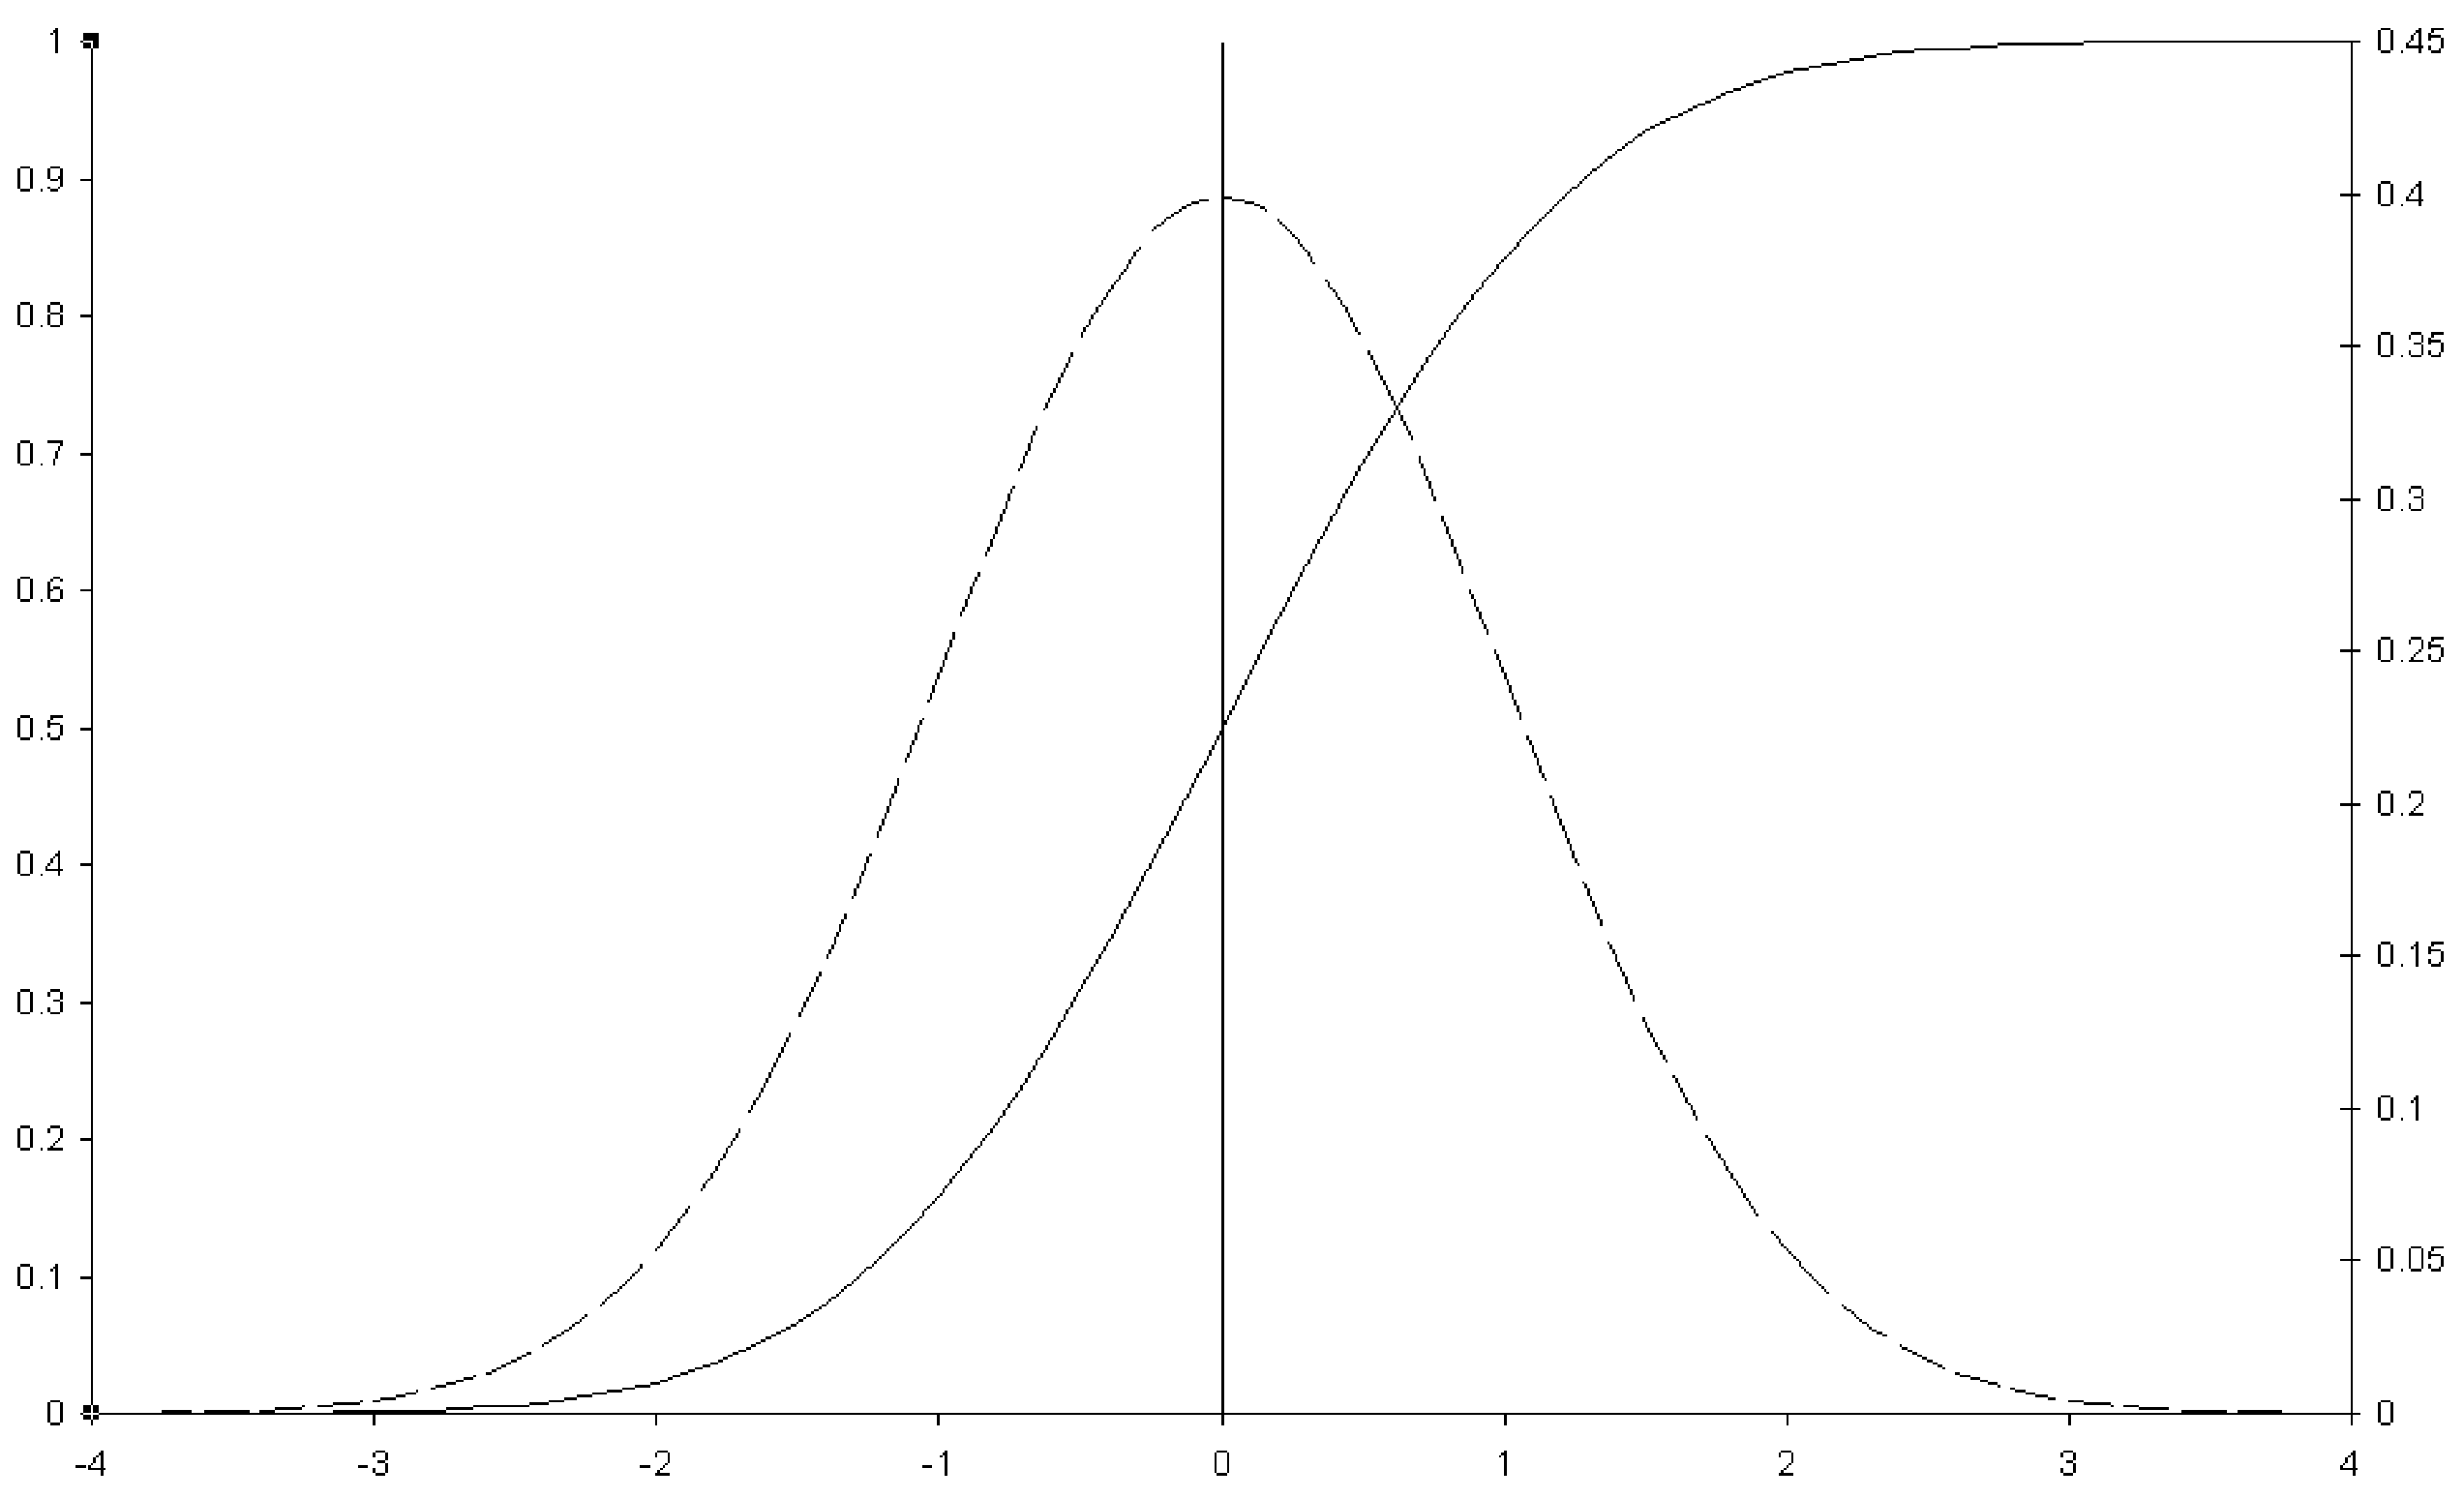
\includegraphics[width=8cm]{Figures/ErrorFunction}
\caption{The error function and the normal distribution}
\label{fig:errorFunction}
\end{figure}
The error function is the integral of the normal distribution. The
error function is used in statistics to evaluate the probability
of finding a measurement larger than a given value when the
measurements are distributed according to a normal distribution.
Figure \ref{sec:errorFunction} shows the familiar bell-shaped
curve of the probability density function of the normal
distribution (dotted line) together with the error function (solid
line).

In medical sciences one calls {\textsl centile} the value of the error
function expressed in percent. For example, obstetricians look
whether the weight at birth of the first born child is located
below the $10^{\mbox{th}}$ centile or above the $90^{\mbox{th}}$
centile to assess a risk factor for a second
pregnancy\footnote{\cf footnote \ref{ft:steer} on page
\pageref{ft:steer}}.

\subsection{Mathematical definitions}
\label{sec:errorFunctionDef} Because it is the integral of the
normal distribution, the error function, $\erf\left(x\right)$,
gives the probability of finding a value lower than $x$ when the
values are distributed according to a normal distribution with
mean 0 and standard deviation 1. The mean and the standard
deviation are explained in section \ref{sec:moments}. This
probability is expressed by the following integral\footnote{In
\cite{AbrSteg} and \cite{Press}, the error function is defined as:
$$\erf\left(x\right)={2 \over \sqrt{\pi}}\int_0^x e^{-{t^2 \over 2
}}dt$$.}:
\begin{equation}
\erf\left(x\right)={1 \over \sqrt{2\pi}}\int_{-\infty}^x e^{-{t^2
\over 2 }}dt
\end{equation}
The result of the error function lies between 0 and 1.

One could carry out the integral numerically, but there exists
several good approximations. The following formula is taken from
\cite{AbrSteg}.
\begin{mainEquation}
\label{eq:erf} \erf\left(x\right)={1 \over \sqrt{2\pi}}e^{-{x^2
\over 2 }}\sum_{i=1}^5 a_i r\left(x\right)^i\mbox{\quad for $x\ge
0$}.
\end{mainEquation}
where
\begin{equation}
\label{eq:erfpol}r\left(x\right)={1 \over {1-0.2316419x}}.
\end{equation}
and
\begin{equation}
\label{eq:erfconst}\left\{ \begin{array}{lr}a_1 =&0.31938153 \\
a_2 =&-0.356563782
\\a_3 =&1.7814779372 \\ a_4 =&-1.821255978 \\ a_5 =&1.330274429
\end{array}\right.
\end{equation}
The error on this formula is better than $7.5\times10^{-8}$ for
negative $x$.
To compute the value for positive values, one uses the fact that:
\begin{mainEquation}
\label{eq:erfneg} \erf\left(x\right)=1-\erf\left(-x\right).
\end{mainEquation}
When dealing with a general Gaussian distribution with average
$\mu$ and standard deviation $\sigma$ it is convenient to define a
generalized error function as:
\begin{equation}
\erf\left(x;\mu,\sigma\right)={1 \over
\sqrt{2\pi\sigma^2}}\int_{-\infty}^x e^{-{{\left(x-\mu\right)}^2
\over 2 \sigma^2}}dt.
\end{equation}
A simple change of variable in the integral shows that the
generalized error function can be obtained from the error function
as:
\begin{mainEquation}
\erf\left(x;\mu,\sigma\right)=\erf\left({x-\mu\over\sigma}\right).
\end{mainEquation}
Thus, one can compute the probability of finding a measurement $x$
within the interval $\left[\mu - t \cdot \sigma,\mu + t \cdot
\sigma\right] $ when the measurements are distributed according to
a Gaussian distribution with average $\mu$ and standard deviation
$\sigma$:
\begin{equation}
\label{eq:normaccept}
\prob\left({\left|x-\mu\right|\over\sigma}\le t\right)=2 \cdot
\erf\left(t\right)-1.\mbox{\quad for $t\ge 0$}.
\end{equation}

\rubrique{Example}
\def\w{2.85}\def\av{3.39}\def\st{0.44}
 Now we can give the answer to the problem of deciding
whether a pregnant woman needs special attention during her second
pregnancy. Let the weight at birth of her first child be $\w\kg$.
and let the duration of her first pregnancy be 39 weeks. In this
case measurements over a representative sample of all births
yielding healthy babies have an average of $\av\kg$ and a standard
deviation of $\st\kg$\footnote{\label{ft:steer}This is the
practice at the department of obstetrics and gynecology of the
Chelsea $\&$ Westminster Hospital of London. The numbers are
reproduced with permission of Prof. P.J. Steer.}. The probability
of having a weight of birth smaller than that of the woman's first
child is:
\begin{eqnarray*}
\prob\left(\mathop{\textrm Weight}\le \w\kg \right) & = &
\erf\left({\w-\av\over\st}\right),\\ & = & 11.2\%.
\end{eqnarray*}
According to current practice, this second pregnancy does not
require special attention.

\subsection{Error function --- Smalltalk implementation}
\label{sec:sterrorfunction} \marginpar{Figure \ref{fig:functions}
with the box {\textbf ErfApproximation} grayed.} The error function is
implemented as a single method for the class Number. Thus,
computing the centile of our preceding example is simply coded as:
\begin{displaycode}{Smalltalk}
| weight average stDev centile |
weight := 2.85.
average := 3.39.
stDev := 0.44.
centile := ((weight - average) / stDev) erf * 100.
\end{displaycode}
If you want to compute the probability for a measurement to lay
within 3 standard deviations from its mean, you need to evaluate
the following expression using equation \ref{eq:normaccept}:
\begin{displaycode}{Smalltalk}
3 errorFunction * 2 - 1.
\end{displaycode}
If one needs to use the error function as a function, one must use
it inside a block closure. In this case one defines a function
object as follows:
\begin{displaycode}{Smalltalk}
| errorFunction |
errorFunction := [:x | x errorFunction].
\end{displaycode}

Listing \ref{lst:errorFunction} shows the Smalltalk implementation
of the error function.

In Smalltalk we are allowed to extend existing classes. Thus, the
public method to evaluate the error function is implemented as a
method of the base class \code{Number}. This method uses the class,
\code{PMErfApproximation}, used to store the constants of equation
\ref{eq:erfconst} and evaluate the formula of equations
\ref{eq:erf} and \ref{eq:erfpol}. In our case, there is no need to
create a separate instance of the class \code{PMErfApproximation}
at each time since all instances would actually be exactly
identical. Thus, the class \code{PMErfApproximation} is a
singleton class. A singleton class is a class, which can only
create a single instance \cite{GoF}. Once the first instance is
created, it is kept in a class instance variable. Any subsequent
attempt to create an additional instance will return a pointer to
the class instance variable holding the first created instance.

One could have implemented all of these methods as class methods
to avoid the singleton class. In Smalltalk, however, one tends to
reserve class method for behavior needed by the structural
definition of the class. So, the use of a singleton class is
preferable. A more detailed discussion of this topic can be found
in \cite{StDesPat}.

\begin{listing}[label=lst:errorFunction]{Smalltalk}
{Smalltalk implementation of the Error function}
Number >> errorFunction
    ^PMErfApproximation new value: self
\end{listing}

\begin{displaycode}{Smalltalk}
Object subclass: #PMErfApproximation
   instanceVariableNames: 'constant series norm'
   classVariableNames: 'UniqueInstance'
   package: 'Math-Core-Distribution'
\end{displaycode}

\begin{displaycode}{Smalltalk}
PMErfApproximation class >> new
    UniqueInstance isNil
        ifTrue: [UniqueInstance := super new initialize].
    ^UniqueInstance
\end{displaycode}

\begin{displaycode}{Smalltalk}
PMErfApproximation >> initialize
    constant := 0.2316419.
    norm := 1 / (Float pi * 2) sqrt.
    series := PMPolynomial coefficients: #( 0.31938153 -0.356563782 
                               1.781477937 -1.821255978 1.330274429). 
\end{displaycode}

\begin{displaycode}{Smalltalk}
PMErfApproximation >> normal: aNumber
   "Computes the value of the Normal distribution for aNumber"

   ^ [ (aNumber squared * -0.5) exp * norm ]
     on: Error
     do: [ :signal | signal return: 0 ]
\end{displaycode}

\begin{displaycode}{Smalltalk}
PMErfApproximation >> value: aNumber
    | t |
    aNumber = 0
        ifTrue: [ ^0.5].
    aNumber > 0
        ifTrue: [ ^1- ( self value: aNumber negated)].
    aNumber < -20
        ifTrue: [ ^0].
    t := 1 / (1 - (constant * aNumber)).
    ^(series value: t) * t * (self normal: aNumber)
\end{displaycode}

\section{Gamma function}
The gamma function is used in many mathematical functions. In this
book, the gamma function is needed to compute the normalization
factor of several probability density functions (\cf sections
\ref{sec:gammadist} and \ref{sec:chitest}). It is also needed to
compute the beta function (\cf section \ref{sec:betafunc}).

\subsection{Mathematical definitions}
\label{sec:gammafunc} The Gamma function is defined by the
following integral, called Euler's integral\footnote{Leonard Euler
to be precise as the Euler family produced many mathematicians.}:
\begin{equation}
\label{eq:gammafunc} \Gamma\left(x\right)=\int_0^\infty t^x
e^{-t}dt
\end{equation}
From equation \ref{eq:gammafunc} a recurrence formula can be
derived:
\begin{equation}
\label{eq:gammarec} \Gamma\left(x+1\right)=x \cdot
\Gamma\left(x\right)
\end{equation}
The value of the Gamma function can be computed for special values
of $x$:
\begin{equation}
\label{eq:gammaval}\left\{
\begin{array}{lr}\Gamma\left(1\right)=1\\\Gamma\left(2\right)=1
\end{array}\right.
\end{equation}
From \ref{eq:gammarec} and \ref{eq:gammaval}, the well-known
relation between the value of the Gamma function for positive
integers and the factorial can be derived:
\begin{equation}
\label{eq:gammafact} \Gamma\left(n\right)=\left(n-1\right)!
\mbox{\quad for $n>0$}.
\end{equation}
The most precise approximation for the Gamma function is given by
a formula discovered by Lanczos \cite{Press}:
\begin{mainEquation}
\label{eq:lanczos} \Gamma\left(x\right)\approx e^{\left(x+{5\over
2}\right)}\left(x+{5\over 2}\right){\sqrt{2\pi}\over x
}\left(c_0+\sum_{n=1}^6{c_n \over x + n}+\epsilon\right)
\end{mainEquation}
where
\begin{equation}
\label{eq:lanczosconst}\left\{ \begin{array}{lrl}c_0
=&1.000000000190015
\\c_1 =&76.18009172947146 \\ c_2 =&-86.50532032941677
\\c_3 =&24.01409824083091 \\ c_4 =&-1.231739572450155
\\ c_5 =&1.208650973866179&\cdot 10^{-3} \\ c_6 =&-5.395239384953&\cdot 10^{-6}
\end{array}\right.
\end{equation}
This formula approximates $\Gamma\left(x\right)$ for $x>1$ with
$\epsilon<2\cdot 10^{-10}$ . Actually, this remarkable formula can
be used to compute the gamma function of any complex number $z$
with $\Re\left(z\right)>1$ to the quoted precision. Combining
Lanczos' formula with the recurrence formula \ref{eq:gammarec} is
sufficient to compute values of the Gamma function for all
positive numbers.

For example, $\Gamma\left({3\over 2}\right)={\sqrt{\pi}\over 2}=
0.886226925452758$ whereas Lanczos formula yields the value
$0.886226925452754$, that is, an absolute error of $4\cdot
10^{-15} $. The corresponding relative precision is almost equal
to the floating-point precision of the machine on which this
computation was made.

Although this is seldom used, the value of the Gamma function for
negative non-integer numbers can be computed using the reflection
formula hereafter:
\begin{equation}
\label{eq:gammaneg} \Gamma\left(x\right)={\pi\over
\Gamma\left(1-x\right) \sin\pi x}
\end{equation}

In summary, the algorithm to compute the Gamma function for any
argument goes as follows:
\begin{enumerate}
  \item If $x$ is a non-positive integer ($x\le0$), raise an exception.
  \item If $x$ is smaller than or equal to 1 ($x<1$), use the recurrence formula \ref{eq:gammarec}.
  \item If $x$ is negative ($x<0$, but non integer), use the reflection
formula \ref{eq:gammaneg}.
  \item Otherwise use Lanczos' formula \ref{eq:lanczos}.
\end{enumerate}

One can see from the leading term of Lanczos' formula that the
gamma function raises faster than an exponential. Thus, evaluating
the gamma function for numbers larger than a few hundreds will
exceed the capacity of the floating number representation on most
machines. For example, the maximum exponent of a double precision
IEEE floating-point number is 1024. Evaluating directly the
following expression:
\begin{equation}
\label{eq:gammaovfl}
  {\Gamma\left(460.5\right)\over\Gamma\left(456.3\right)}
\end{equation}
will fail since $\Gamma\left(460.5\right)$ is larger than
$10^{1024}$. Thus, its evaluation yields a floating-point overflow
exception. It is therefore recommended to use the logarithm of the
gamma function whenever it is used in quotients involving large
numbers. The expression of equation \ref{eq:gammaovfl} is then
evaluated as:
\begin{equation}
  \exp\left[\ln\Gamma\left(460.5\right)-\ln\Gamma\left(456.3\right)\right]
\end{equation}
which yield the result $1.497\cdot 10^{11}$. That result fits
comfortably within the floating-point representation.

For similar reasons the leading factors of Lanczos formula are
evaluated using logarithms in both implementations.

\subsection{Gamma function --- Smalltalk implementation}
\marginpar{Figure \ref{fig:functions} with the box {\textbf
LanczosFormula} grayed.} Like the error function, the gamma
function is implemented as a single method of the class {\texttt
Number}. Thus, computing the gamma function of 2.5 is simply coded
as:
\begin{listing}{Smalltalk}
2.5 gamma
\end{listing}
To obtain the logarithm of the gamma function, you need to
evaluate the following expression:
\begin{listing}{Smalltalk}
2.5 logGamma
\end{listing}

Listing \ref{ls:gammafunc} shows the Smalltalk implementation of the gamma
function.

Here, the gamma function is implemented with two methods: one for
the class {\texttt Integer} and one for the class {\texttt Float}.
Otherwise, the scheme to define the gamma function is similar to
that of the error function. Please refer to section
\ref{sec:sterrorfunction} for detailed explanations.

Since the method factorial is already defined for integers in the
base classes, the gamma function has been defined using equation
\ref{eq:gammafact} for integers. An error is generated if one
attempts to compute the gamma function for non-positive integers.
The class {\texttt Number} delegates the computation of Lanczos'
formula to a singleton class. This is used by the non-integer
subclasses of {\texttt Number}: {\texttt Float} and {\texttt Fraction}.

The execution time to compute the gamma function for floating
argument given in Table \ref{tb:speed} in section \ref{sec:speed}.
\begin{listing}[label=ls:gammafunc]{Smalltalk}
{Smalltalk implementation of the gamma function}
$$\halign{ #\hfil&\quad#\hfil\cr {\sl Class}& {\Large\bf Integer}\cr
{\sl Subclass of }&{\tt Number}\cr\noalign{\vskip 1ex}
}$$


Instance methods
{\parskip 1ex\par\noindent}
{\bf gamma}
\begin{verbatim}
    self > 0
        ifFalse: [ ^self error: 'Attempt to compute the Gamma 
        function of a non-positive integer'].
    ^( self - 1) factorial
\end{verbatim}


$$\halign{ #\hfil&\quad#\hfil\cr {\sl Class}& {\Large\bf Number}\cr
{\sl Subclass of }&{\tt Magnitude}\cr\noalign{\vskip 1ex}
}$$


Instance methods
{\parskip 1ex\par\noindent}
{\bf gamma}
\begin{verbatim}
    ^self > 1
        ifTrue: [ ^DhbLanczosFormula new gamma: self]
        ifFalse:[ self < 0
                     ifTrue: [ Float pi / ( ( Float pi * self) sin * ( 1 - self) gamma)]
                     ifFalse:[ ( DhbLanczosFormula new gamma: (self + 1)) / self]
                    ]
\end{verbatim}
{\bf logGamma}
\begin{verbatim}
    ^self > 1
        ifTrue: [ DhbLanczosFormula new logGamma: self]
        ifFalse: [ self > 0
                      ifTrue: [ ( DhbLanczosFormula new logGamma: (self + 1)) - self ln ]
                      ifFalse: [ ^self error: 'Argument for the log gamma function
                         must be positive']
                    ]
\end{verbatim}


$$\halign{ #\hfil&\quad#\hfil\cr {\sl Class}& {\Large\bf DhbLanczosFormula}\cr
{\sl Subclass of }&{\tt Object}\cr\noalign{\vskip 1ex}

{\sl Instance variable names:}&\parbox[t]{4 in}{\tt  coefficients sqrt2Pi }\cr\noalign{\vskip 1ex}
{\sl Class variable names:}&\parbox[t]{4 in}{\tt  UniqueInstance }\cr\noalign{\vskip 1ex}}$$


Class methods
{\parskip 1ex\par\noindent}
{\bf new}
\begin{verbatim}
    UniqueInstance isNil
        ifTrue: [ UniqueInstance := super new initialize ].
    ^ UniqueInstance
\end{verbatim}

Instance methods
{\parskip 1ex\par\noindent}
{\bf gamma:} {\tt aNumber}
\begin{verbatim}
    ^ (self leadingFactor: aNumber) exp * (self series: aNumber) 
        * sqrt2Pi / aNumber
\end{verbatim}
{\bf initialize}
\begin{verbatim}
    sqrt2Pi := ( Float pi * 2) sqrt.
    coefficients := #( 76.18009172947146 -86.50532032941677 
           24.01409824083091 -1.231739572450155 0.1208650973866179e-2 
           -0.5395239384953e-5).
    ^ self
\end{verbatim}
{\bf leadingFactor:} {\tt aNumber}
\begin{verbatim}
    | temp |
    temp := aNumber + 5.5.
    ^ (temp ln * ( aNumber + 0.5) - temp)
\end{verbatim}
{\bf logGamma:} {\tt aNumber}
\begin{verbatim}
    ^ (self leadingFactor: aNumber) + ((self series: aNumber) 
    * sqrt2Pi / aNumber) ln
\end{verbatim}
{\bf series:} {\tt aNumber}
\begin{verbatim}
    | term |
    term := aNumber.
    ^coefficients inject: 1.000000000190015
                        into: [ :sum :each | term := term + 1. each / term + sum ]
\end{verbatim}


\end{listing}

\section{Beta function}
\label{sec:betafunc} The beta function is directly related to the
gamma function. In this book, the beta function is needed to
compute the normalization factor of several probability density
functions (\cf sections \ref{sec:Ftest}, \ref{sec:ttest} and
\ref{sec:betadist}).
\subsection{Mathematical definitions}
The beta function is defined by the following integral:
\begin{equation}
\label{eq:betaint} B\left(x,y\right)=\int_0^1
t^{x-1}\left(1-t\right)^{y-1}dt
\end{equation}
The beta function is related to the gamma function with the
following relation:
\begin{equation}
B\left(x,y\right)={\Gamma\left(x\right)\Gamma\left(y\right)\over\Gamma\left(x+y\right)}
\end{equation}
Thus, computation of the beta function is directly obtained from
the gamma function. As evaluating the gamma function might
overflow the floating-point exponent (\cf discussion at the end of
section \ref{sec:gammafunc}), it is best to evaluate the above
formula using the logarithm of the gamma function.

\subsection{Beta function --- Smalltalk implementation}
\marginpar{Figure \ref{fig:functions} with the box {\textbf
LanczosFormula} grayed.} Like the error and gamma functions, the
gamma function is implemented as a single method of the class {\texttt
Number}. Thus, computing the beta function of 2.5 and 5.5 is
simply coded as:
\begin{listing}{Smalltalk}
2.5 beta: 5.5
\end{listing}

Computing the logarithm of the beta function of
2.5 and 5.5 is simply coded as:
\begin{listing}{Smalltalk}
2.5 logBeta: 5.5
\end{listing}
Listing \ref{ls:betafunc} shows the
implementation of the beta function in Smalltalk.

\begin{listing}[label=ls:betafun]{Smalltalk}
{Smalltalk implementation of the beta function}
$$\halign{ #\hfil&\quad#\hfil\cr {\sl Class}& {\Large\bf Number}\cr
{\sl Subclass of }&{\tt Magnitude}\cr\noalign{\vskip 1ex}
}$$


Instance methods
{\parskip 1ex\par\noindent}
{\bf beta:} {\tt aNumber}
\begin{verbatim}
    ^ (self logBeta: aNumber) exp
\end{verbatim}
{\bf logBeta:} {\tt aNumber}
\begin{verbatim}
    ^ self logGamma + aNumber logGamma - ( self + aNumber) logGamma
\end{verbatim}


\end{listing}

%\ifx\wholebook\relax\else\end{document}\fi

%\ifx\wholebook\relax\else
%\documentclass[twoside]{book}
%\usepackage[active]{srcltx}
%\usepackage[LY1]{fontenc}
%\usepackage{url}
\makeatletter
\def\url@leostyle{%
  \@ifundefined{selectfont}{\def\UrlFont{\sf}}{\def\UrlFont{\sffamily}}}
\makeatother
% Now actually use the newly defined style.
\urlstyle{leo}

\usepackage{graphicx}
\def\etc{{\textit{etc}}}
\def\eg{{\textit{e.g.}}}
\def\ie{{\textit{i.e.}}}
\def\cf{{\textit{c.f.}}\ }
\def\erf{\mathop{\textrm{erf}}}
\def\sign{\mathop{\textrm{sign}}}
\def\prob{\mathop{\textrm{Prob}}}
\def\var{\mathop{\textrm{var}}}
\def\mod{\mathop{\textrm{mod}}}
\def\cor{\mathop{\textrm{cor}}}
\def\cov{\mathop{\textrm{cov}}}
\def\cl{\mathop{\textrm{CL}}}
\def\kg{\mathop{\textrm{Kg}}}
\def\patstyle#1{{\textsc #1}}
\def\th{^{\mathop{\textrm{th}}}}
%\def\st#1{^{\mathop{\rm #1}}}
\def\note#1{\begin{quote}{\textbf{Note:}} #1\end{quote}}
\def\braket#1{\left\langle #1\right\rangle}
\def\order#1{\let\o=#1$\mathcal{O}$\ifx\o 1$\left(n\right)$\else$\left(n^{#1}\right)$\fi}
%\newtheorem{privListing}{Listing}[chapter]
%\newenvironment{listing}{\vskip 3ex\hrule\vskip 1ex\begin{privListing}}{\end{privListing}\hrule\vskip 1ex}
\newtheorem{privExample}{Code example}[chapter]
\newenvironment{codeExample}{\begin{privExample}\begin{quote}\tt}{\end{quote}\end{privExample}}
\def\relboxl#1#2{\hbox to #1\hsize{#2\hfil}}
\def\relboxc#1#2{\hbox to #1\hsize{\hfil #2\hfil}}
\def\relboxr#1#2{\hbox to #1\hsize{\hfil #2}}
\def\transpose#1{\textbf{#1}^{\mathop\textrm{T}}}
\def\inverse#1{\textbf{#1}^{-1}}
%\def\tm{$^{\mathop{\rm TM}}$}
\def\tm{ }
\newenvironment{mainEquation}{\marginpar[\vspace{3 ex} Main
equation$\Rightarrow$]{\vspace{3 ex}$\Leftarrow$Main
equation}\begin{equation}}{\end{equation}}
\def\rubrique#1{\paragraph{#1}\hfil\par\noindent}

%\begin{document}
%\fi

\chapter{Interpolation}
\label{ch:interpolation}
\begin{flushright}
{\textsl On ne peut pr\'evoir les choses qu'apr\`es qu'elles sont
arriv\'ees.}\footnote{One can predict things only after they have
occurred.}\\ Eug\`ene Ionesco
\end{flushright}
\vspace{1 ex} Interpolation is a technique allowing the estimation
of a function over the range covered by a set of points at which
the function's values are known. These points are called the {\textsl
sample} points. Interpolation is useful to compute a function
whose evaluation is highly time consuming: with interpolation it
suffices to compute the function's values for a small number of
well-chosen sample points. Then, evaluation of the function
between the sample points can be made with interpolation.

Interpolation can also be used to compute the value of the inverse
function, that is finding a value $x$ such that
$f\left(x\right)=c$ where $c$ is a given number, when the function
is known for a few sample points bracketing the sought value.
People often overlook this easy and direct computation of the
inverse function.

Interpolation is often used interchangeably with extrapolation.
This is not correct, however. Extrapolation is the task of
estimating a function outside of the range covered by the sample
points. If no model exists for the data extrapolation is just
gambling. Methods exposed in this chapter should not be used for
extrapolation.

Interpolation should not be mistaken with function (or curve)
fitting. In the case of interpolation the sample points purely
determine the interpolated function. Function fitting allows
constraining the fitted function independently from the sample
points. As a result fitted functions are more stable than
interpolated functions especially when the supplied values are
subject to fluctuations coming from rounding or measurement
errors. Fitting is discussed in chapter \ref{ch:estimation}.

\section{General remarks}
\label{sec:interpolgen} There are several methods of
interpolation. One difference is the type of function used. The
other is the particular algorithm used to determine the function.
For example, if the function is periodic, interpolation can be
obtained by computing a sufficient number of coefficients of the
Fourier series for that function.

In the absence of any information about the function, polynomial
interpolation gives fair results. The function should not have any
singularities over the range of interpolation. In addition there
should not be any pole in the vicinity of the complex plane near
the portion of the real axis corresponding to the range of
interpolation. If the function has singularities it is recommended
to use rational functions --- that is the quotient of two
polynomials --- instead \cite{Press}.

In this chapter we discuss 3 interpolation functions: Lagrange
interpolation polynomial, a diagonal rational function
(Bulirsch-Stoer interpolation) and cubic spline. Furhermore, we
show 3 different implementation of the Lagrange interpolation
polynomial: direct implementation of Lagrange's formula, Newton's
algorithm and Neville's algorithm.
\begin{figure}
\label{cls:interpolation}
\centering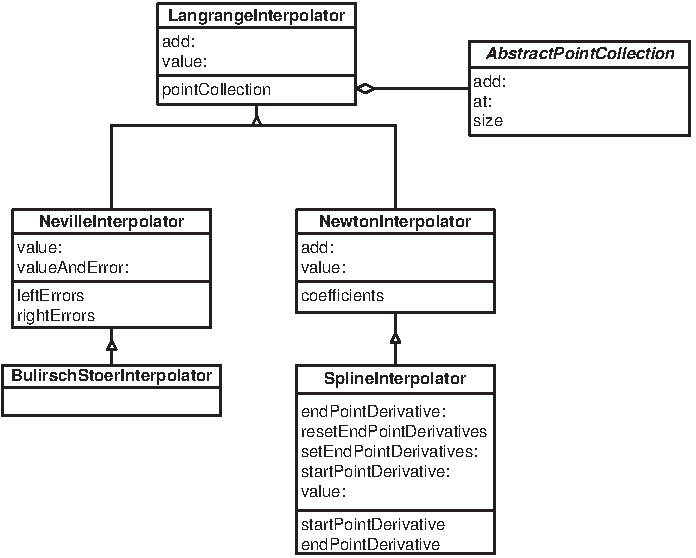
\includegraphics[width=11cm]{Figures/InterpolationClassDiagram}
\caption{Class diagram for the interpolation classes}
\end{figure}
Figure \ref{cls:interpolation} shows how the classes corresponding
to the different interpolation methods described in this chapter
are related to each other.

\rubrique{Definition} The {\textit Lagrange interpolation polynomial}
is the unique polynomial of minimum degree going through the
sample points. The degree of the polynomial is equal to the number
of supplied points minus one. A diagonal rational function is the
quotient of two polynomials where the degree of the polynomial in
the numerator is at most equal to that of the denominator. Cubic
spline uses piece-wise interpolation with polynomials but limits
the degree of each polynomial to 3 (hence the adjective cubic).

\rubrique{Examples} Before selecting an interpolation method the
user must investigate the validity of the interpolated function
over the range of its intended use. Let us illustrate this remark
with an example from high-energy physics, that, in addition, will
expose the limitation of the methods exposed in this chapter.

\begin{figure}
\label{fig:landauinterpol}
\centering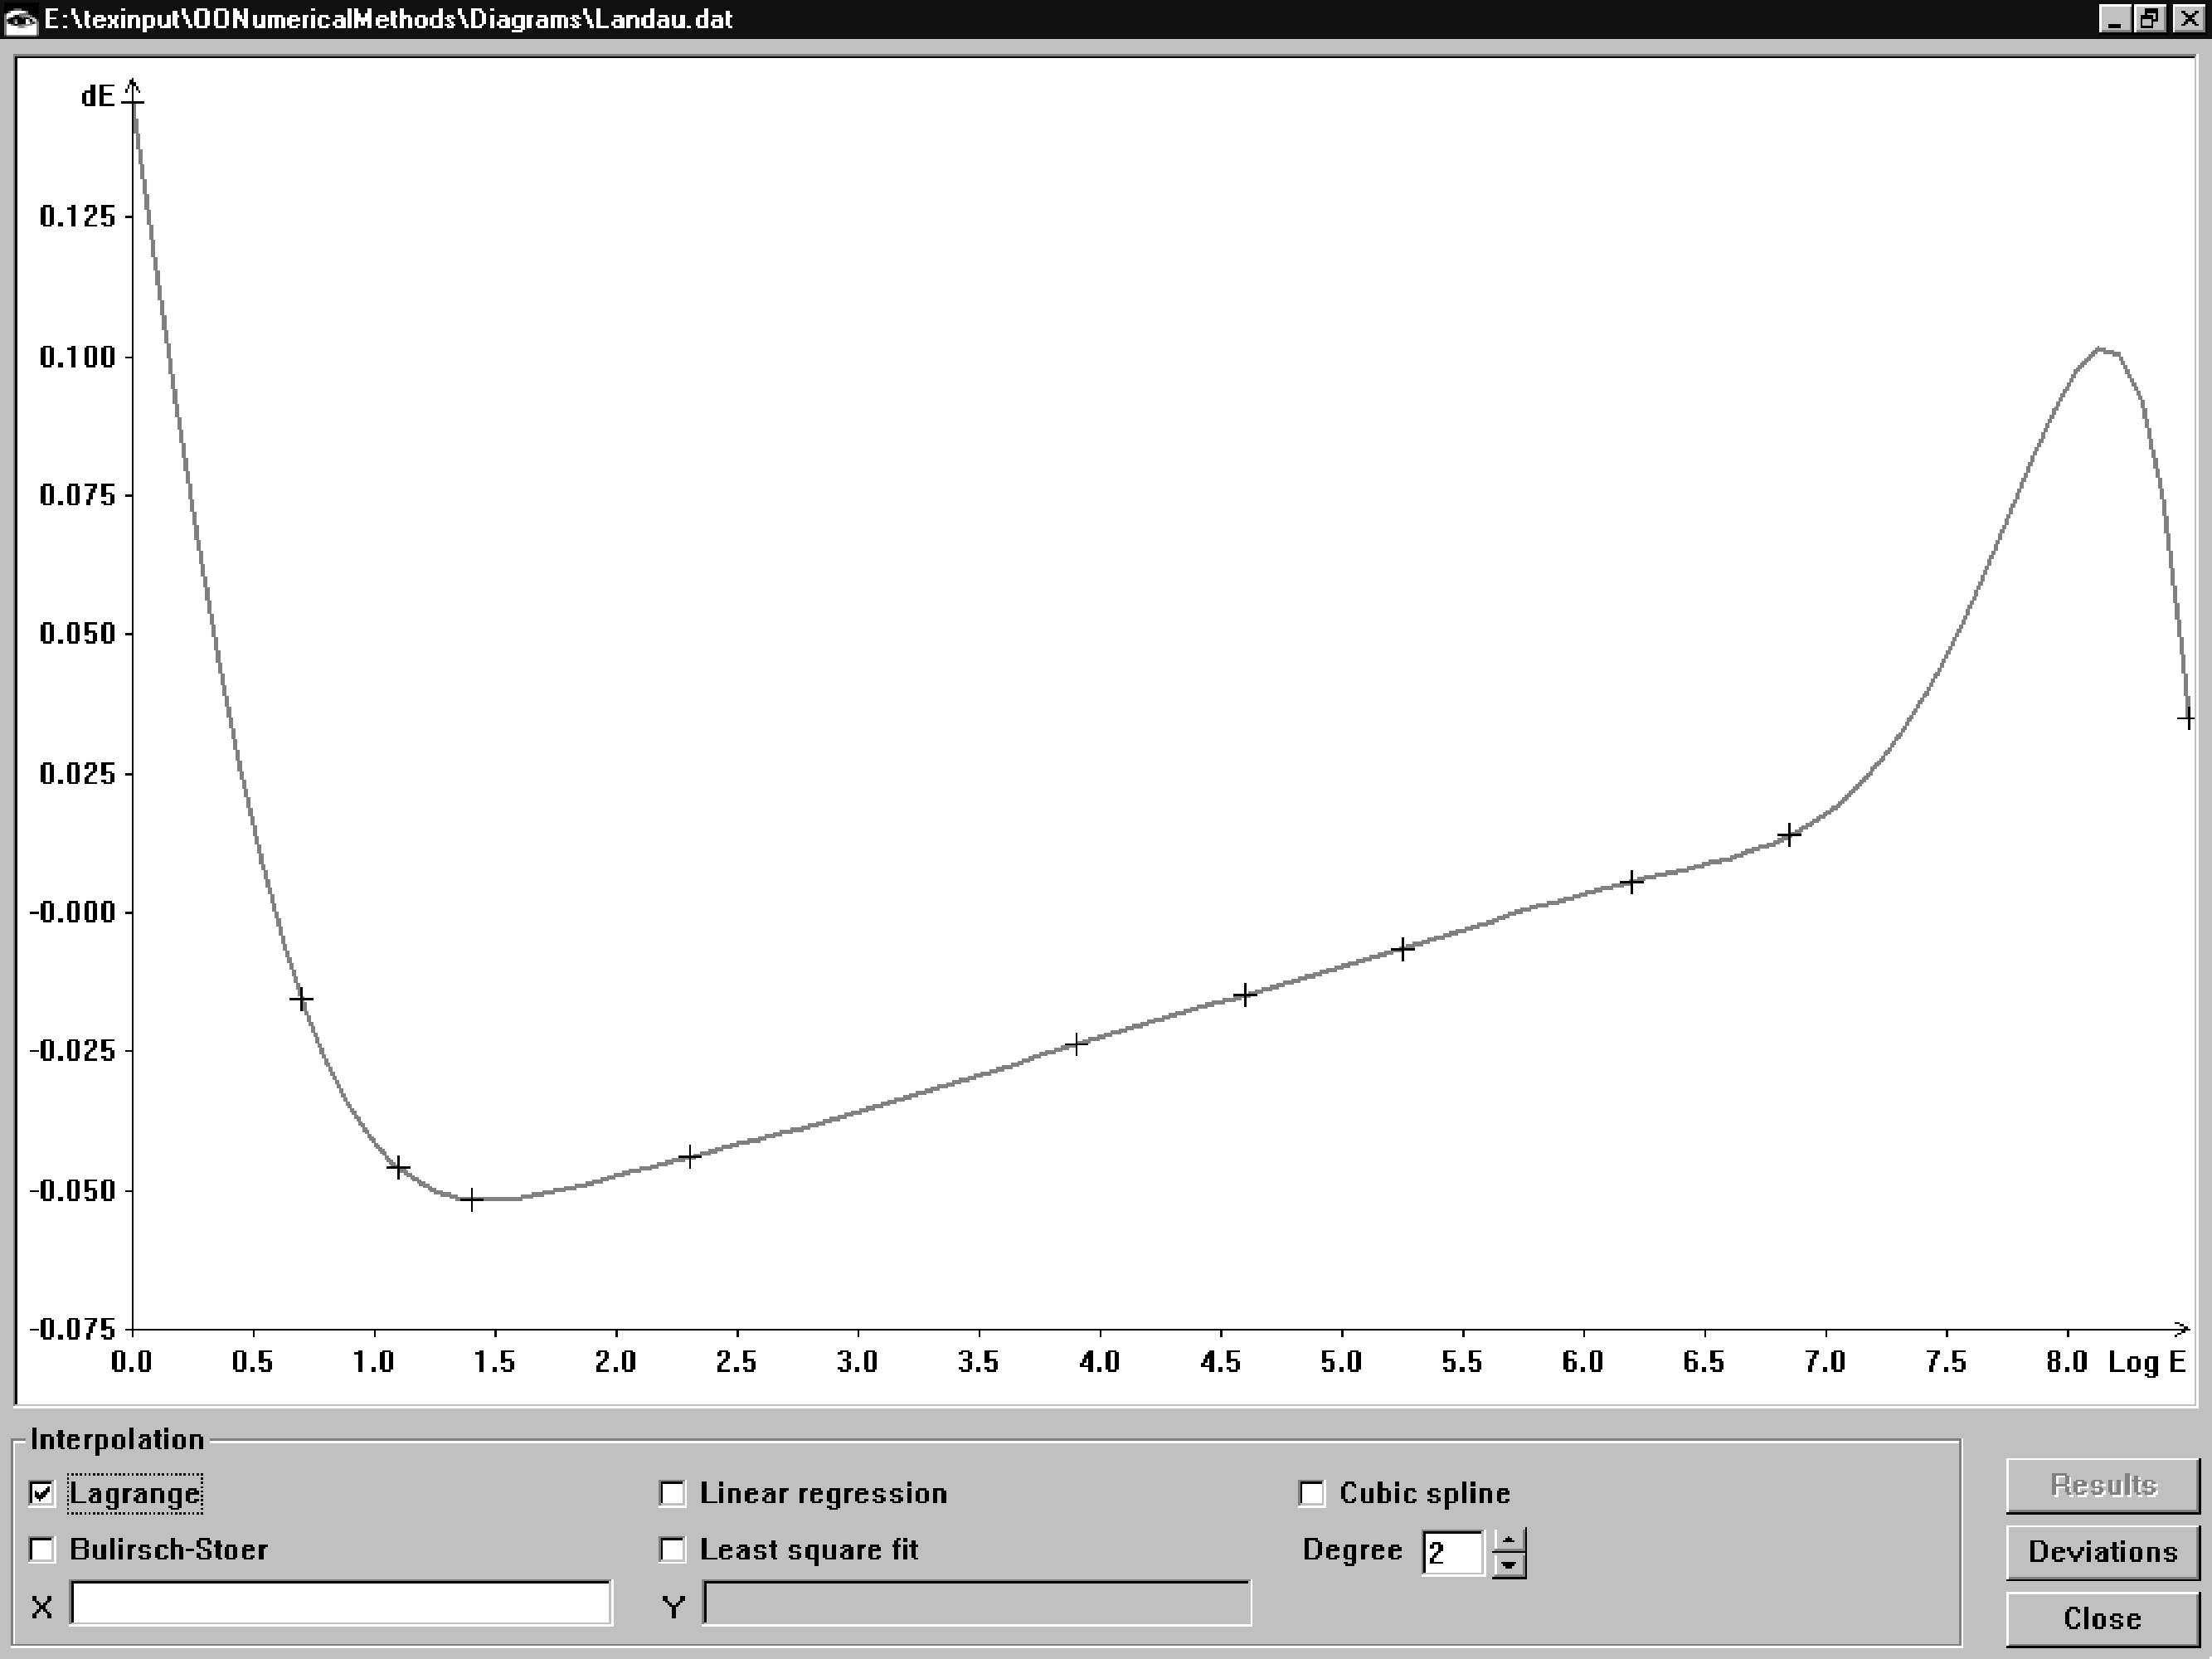
\includegraphics[width=12cm]{Figures/Lagrange}
\caption{Example of interpolation with the Lagrange interpolation
polynomial}
\end{figure}
Figure \ref{fig:landauinterpol} shows sample points --- indicated
by crosses --- representing correction to the energy measured
within a gamma ray detector made of several densely packed
crystals. The energy is plotted on a logarithmic scale. The
correction is caused by the absorption of energy in the wrapping
of each crystal. The sample points were computed using a
simulation program\footnote{This program - EGS written by Ralph
Nelson of the Stanford Linear Accelerator Center (SLAC) -
simulates the absorption of electromagnetic showers inside matter.
Besides being used in high-energy physics this program is also
used in radiology to dimension detectors of PET scanners and other
similar radiology equipment.}, each point requiring several hours
of computing time. Interpolation over these points was therefore
used to allow a quick computation of the correction at any energy.
This is the main point of this example: the determination of each
point was expensive in terms of computing time, but the function
represented by these points is continuous enough to be
interpolated. The simulation program yields results with good
precision so that the resulting data are not subjected to
fluctuation.

The gray thick line in figure \ref{fig:landauinterpol} shows the
Lagrange interpolation polynomial obtained from the sample points.
It readily shows limitations inherent to the use of interpolation
polynomials. The reader can see that for values above 6.5 ---
corresponding to an energy of 500 MeV --- the interpolated
function does not reproduce the curve corresponding to the sample
points. In fact, above 4.0 --- that is,  50 MeV on the scale of
figure \ref{fig:landauinterpol} --- the correction is expected to
be a linear function of the logarithm of the energy.

\begin{figure}
\label{fig:interpolex2}
\centering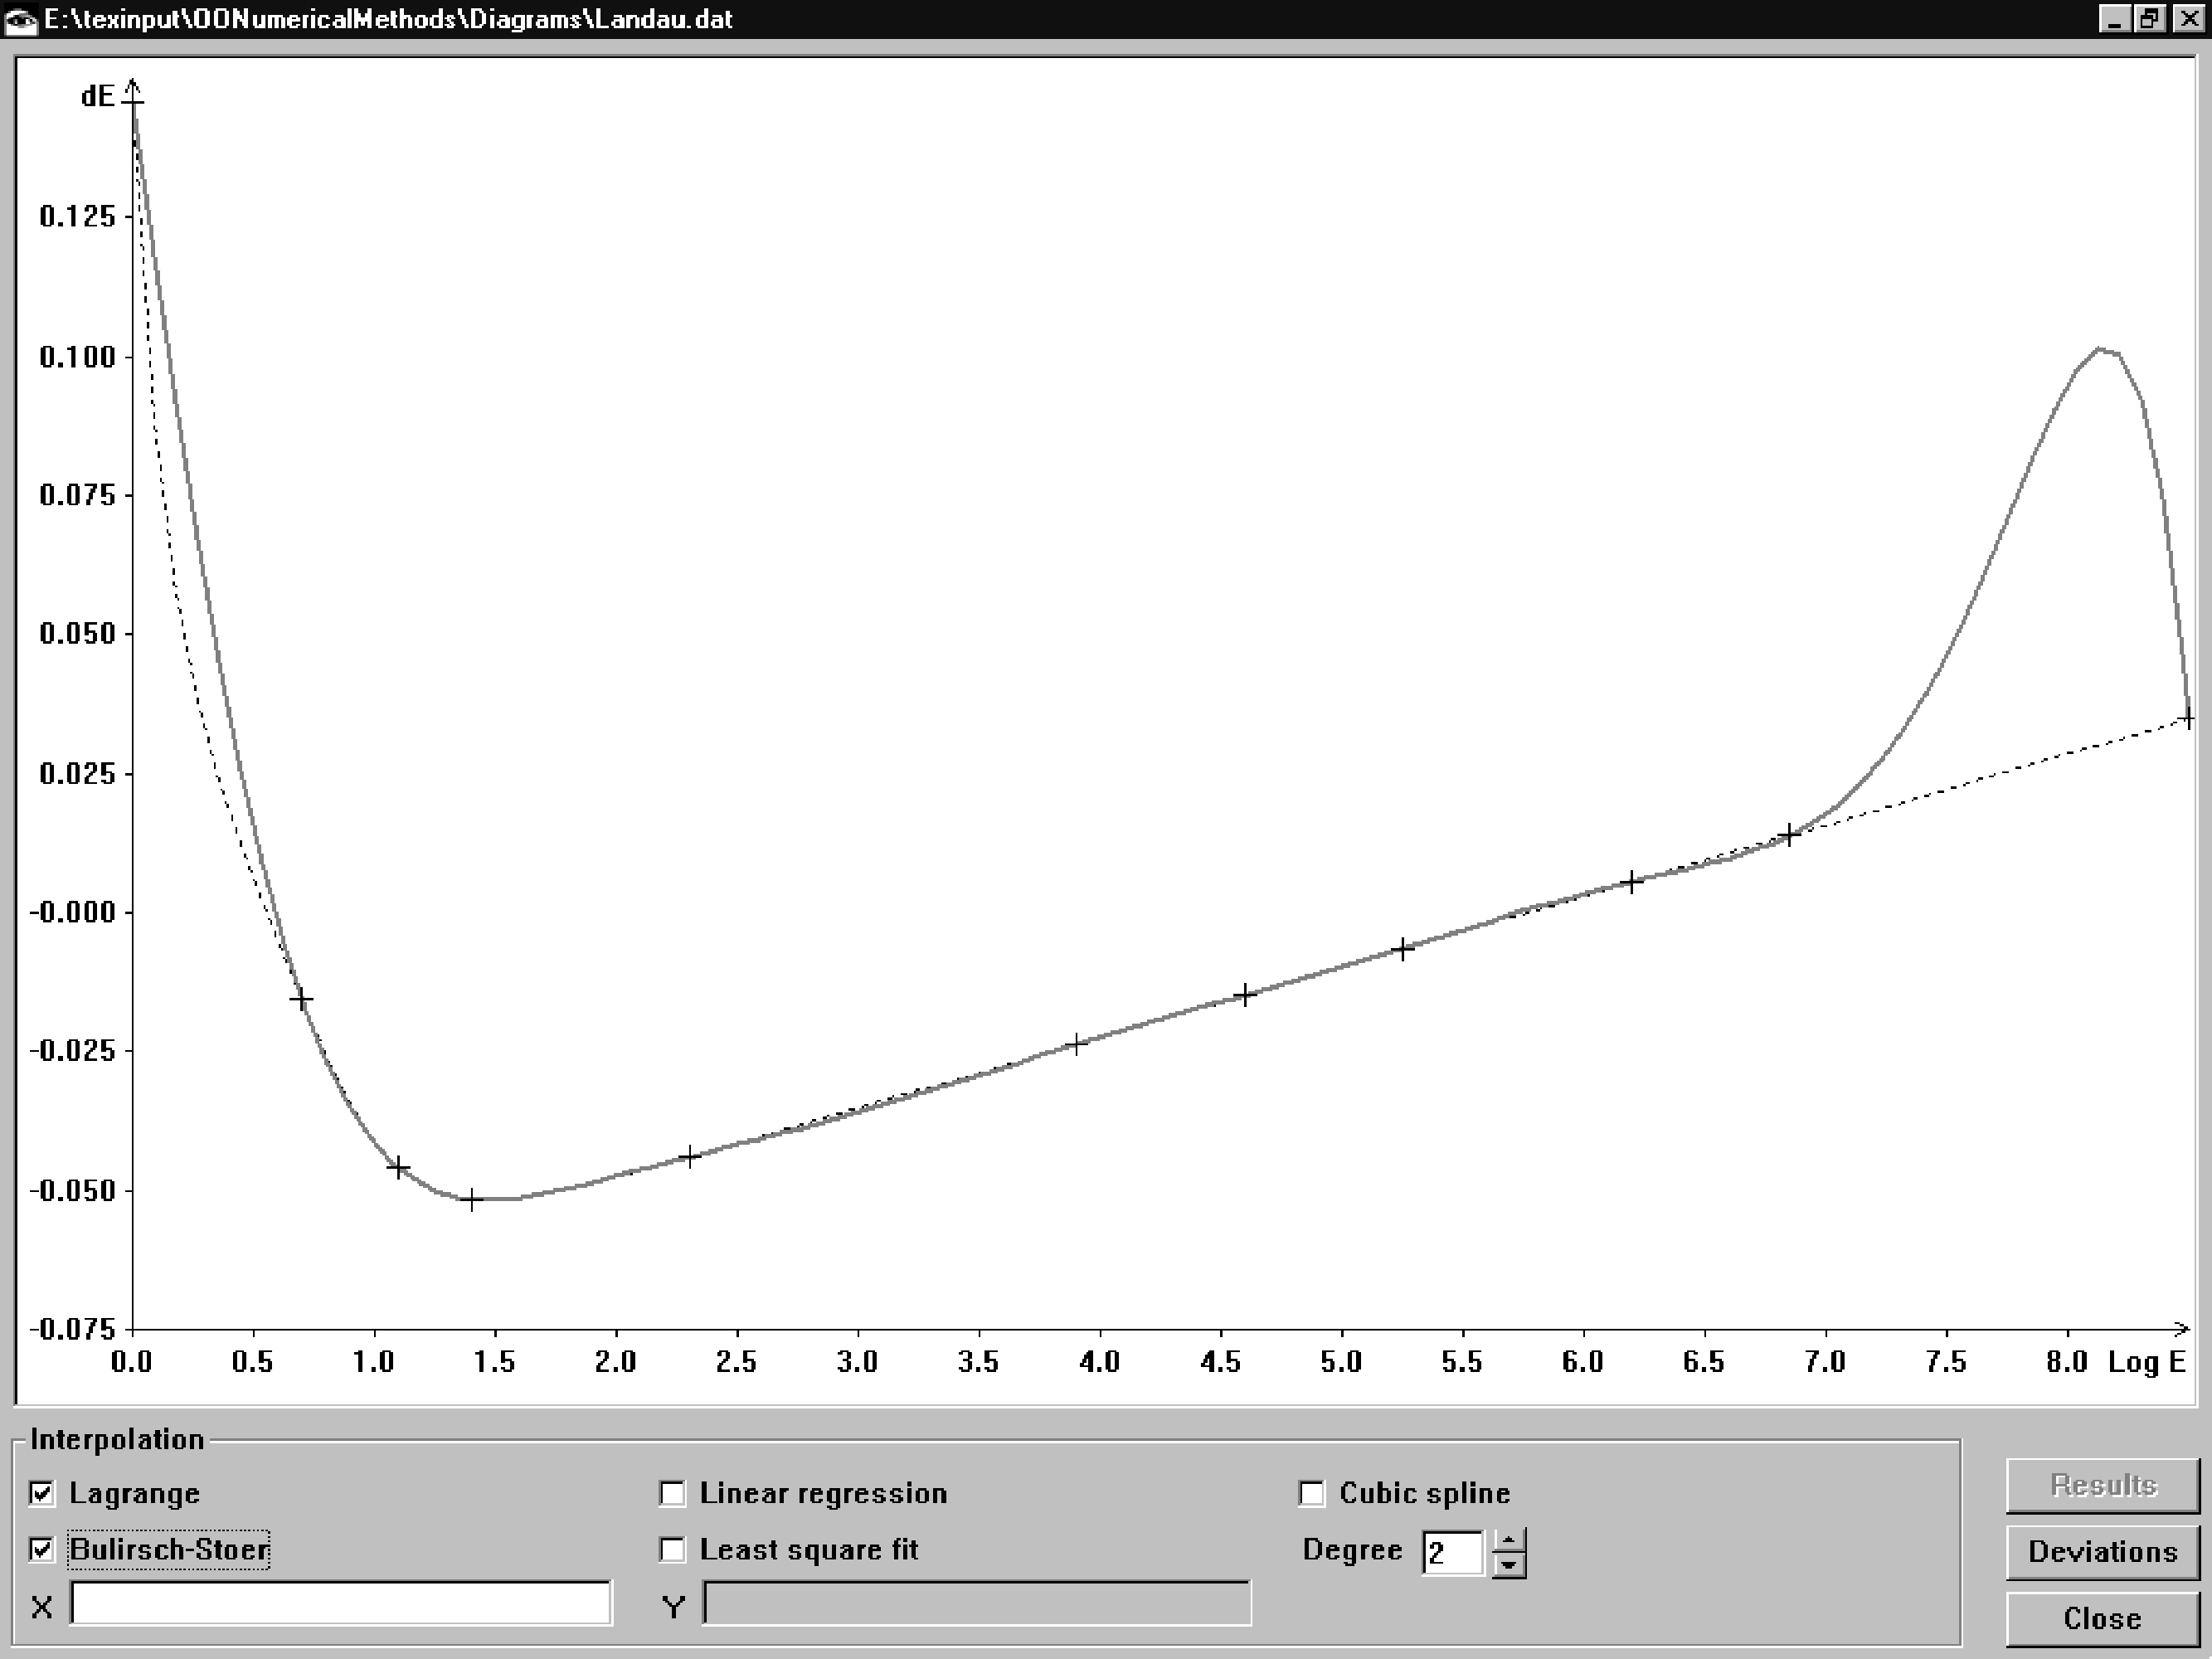
\includegraphics[width=12cm]{Figures/LagrangeVsRational}
\caption{Comparison between Lagrange interpolation and
interpolation with a rational function}
\end{figure}
Figure \ref{fig:interpolex2} shows a comparison between the
Lagrange interpolation polynomial (gray thick line) and
interpolation with a rational function (black dotted line) using
the same sample points as in figure \ref{fig:landauinterpol}. The
reader can see that, in the high-energy region (above 4 on the
scale of figure \ref{fig:interpolex2}) the rational function does
a better job than the Lagrange polynomial. Between the first two
points, however, the rational function fails to reproduce the
expected behavior.

\begin{figure}
\label{fig:interpolex3}
\centering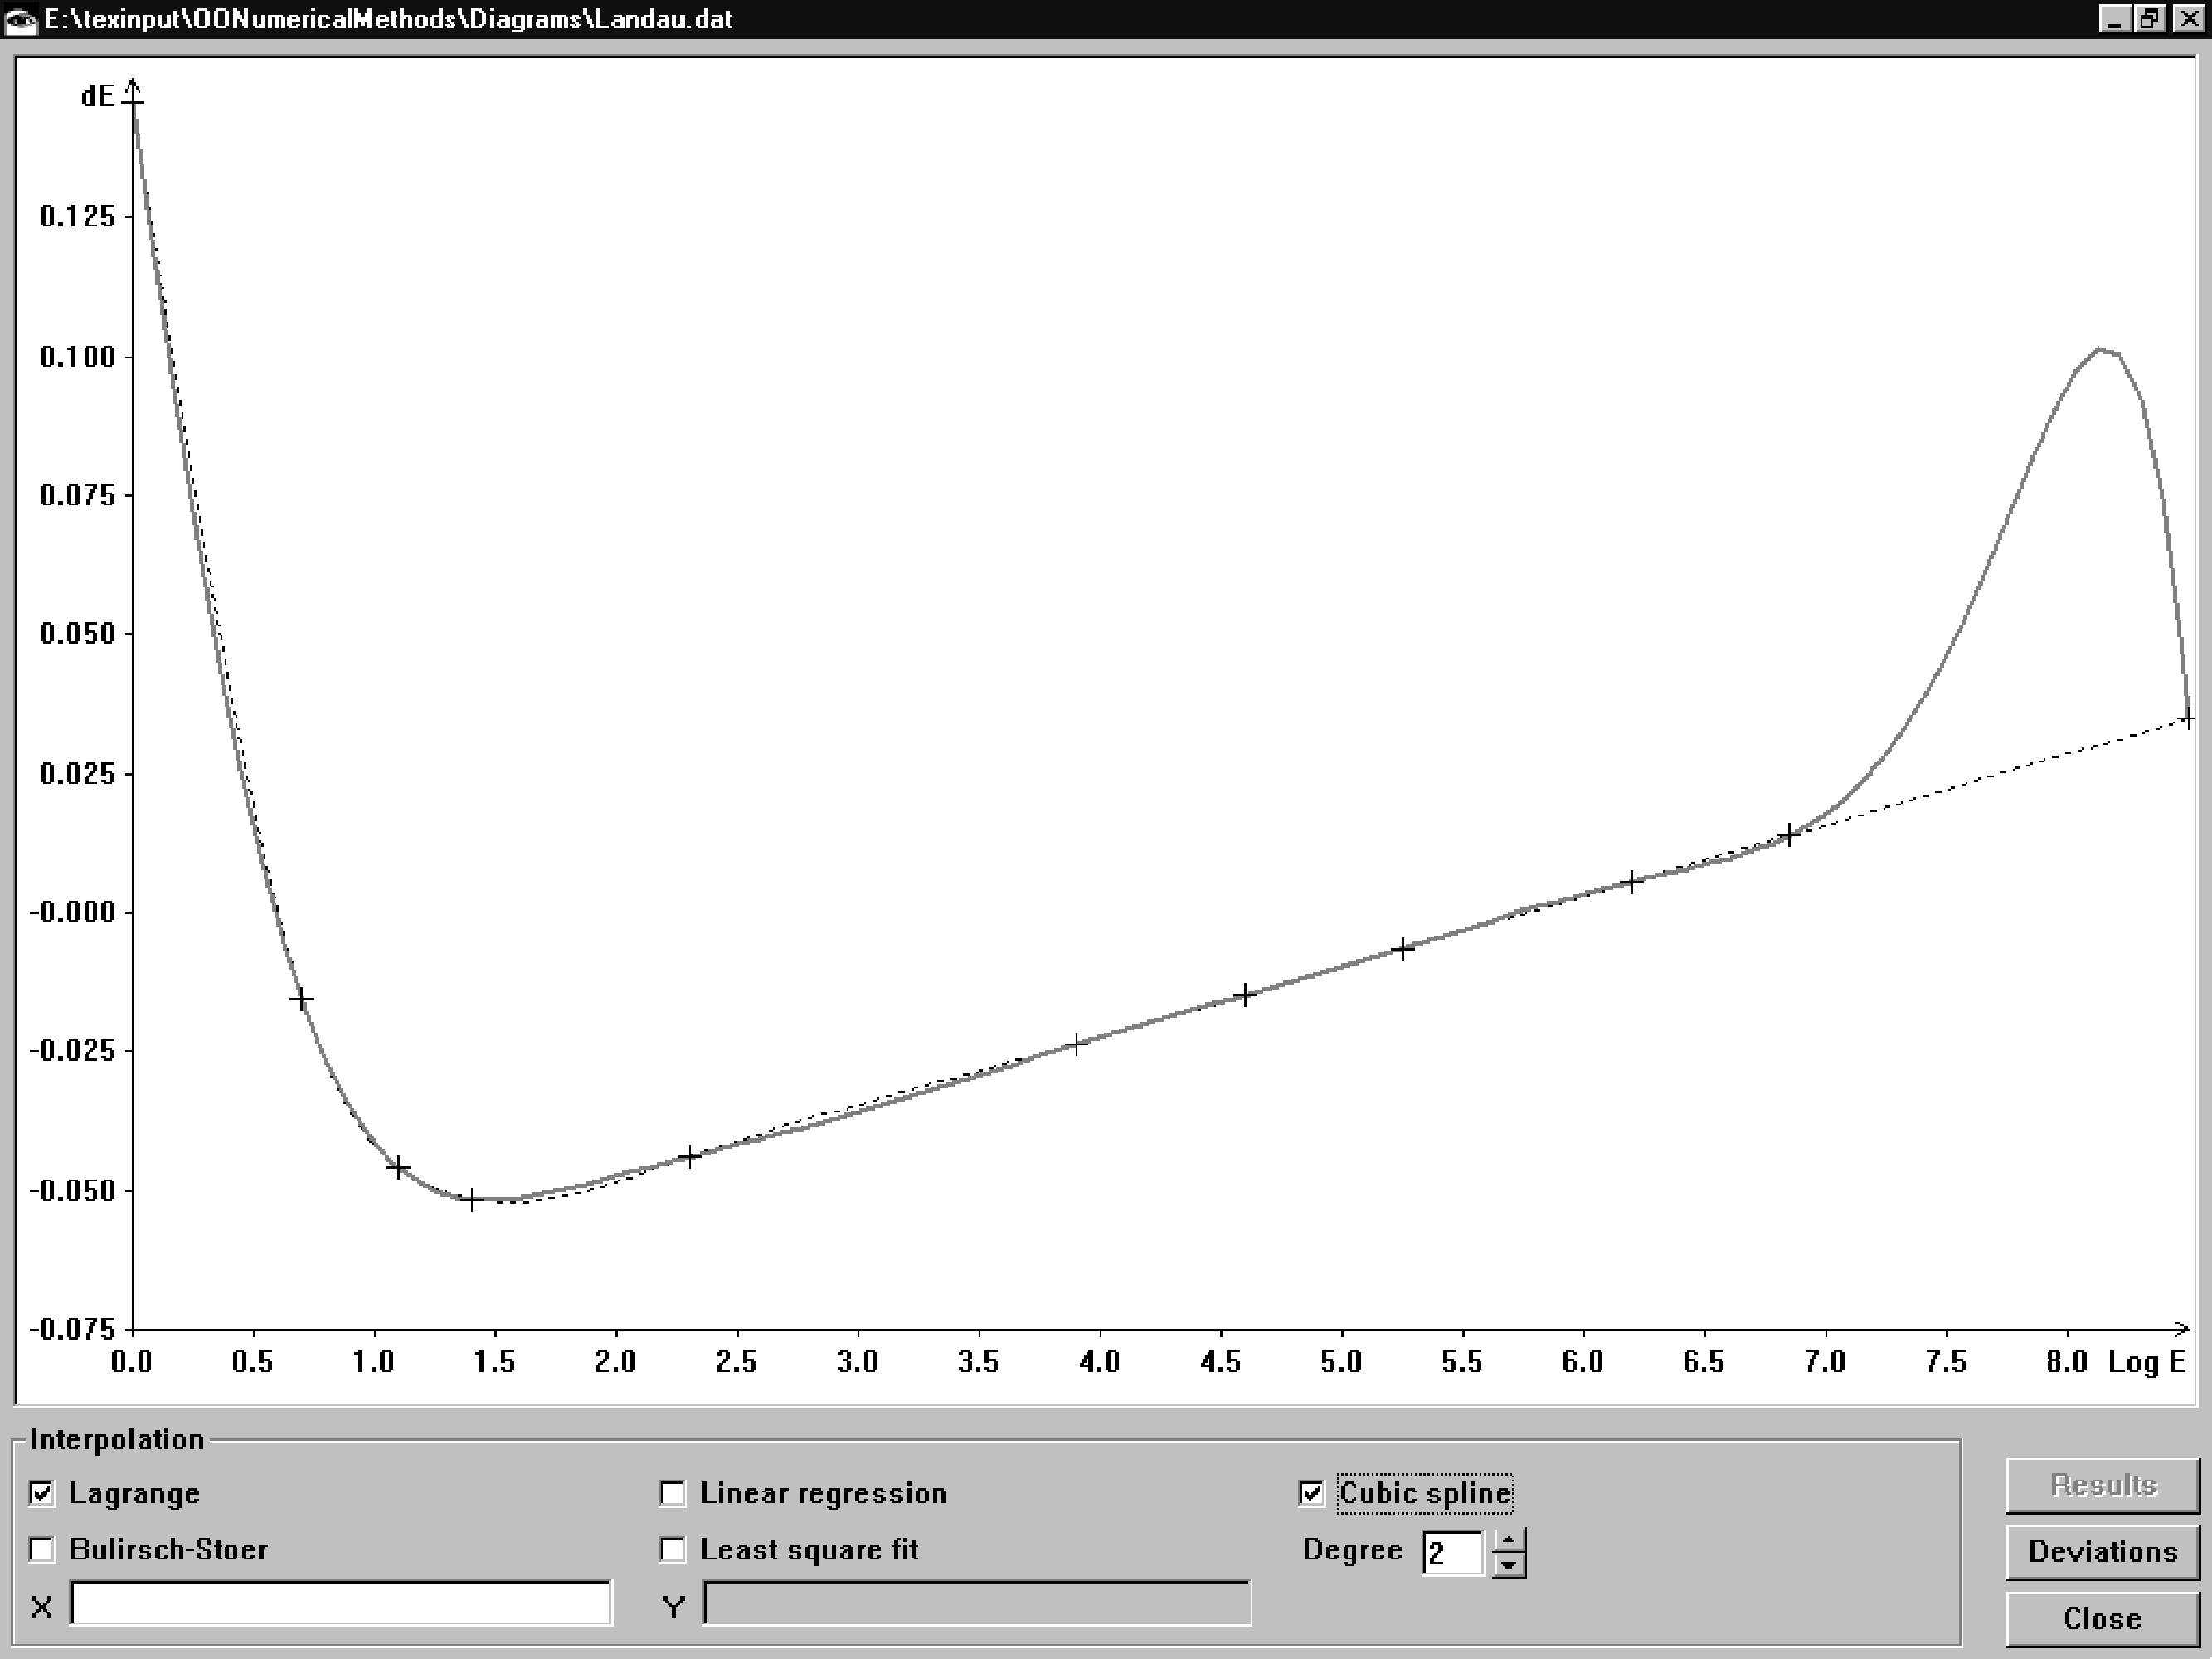
\includegraphics[width=12cm]{Figures/LagrangeVsSpline}
\caption{Comparison of Lagrange interpolation and cubic spline}
\end{figure}
Figure \ref{fig:interpolex3} shows a comparison between the
Lagrange interpolation polynomial (gray thick line) and cubic
spline interpolation (black dotted line) using the same sample
points as in figure \ref{fig:landauinterpol}. The reader can see
that, in the high-energy region (above 4 on the scale of figure
\ref{fig:interpolex2}) the cubic spline does a better job than the
Lagrange polynomial. In fact, since the dependence is linear over
that range, the cubic spline reproduces the theoretical dependence
exactly. In the low energy region, however, cubic spline
interpolation fails to reproduce the curvature of the theoretical
function because of the limitation of the polynomial's degree.

A final example shows a case where interpolation should not be
used. Here the sample points represent the dependence of the
probability that a coin mechanism accepts a wrong coin as a
function of an adjustable threshold. The determination of each
point requires 5-10 minutes of computing time.
\begin{figure}
\label{fig:interpolex4}
\centering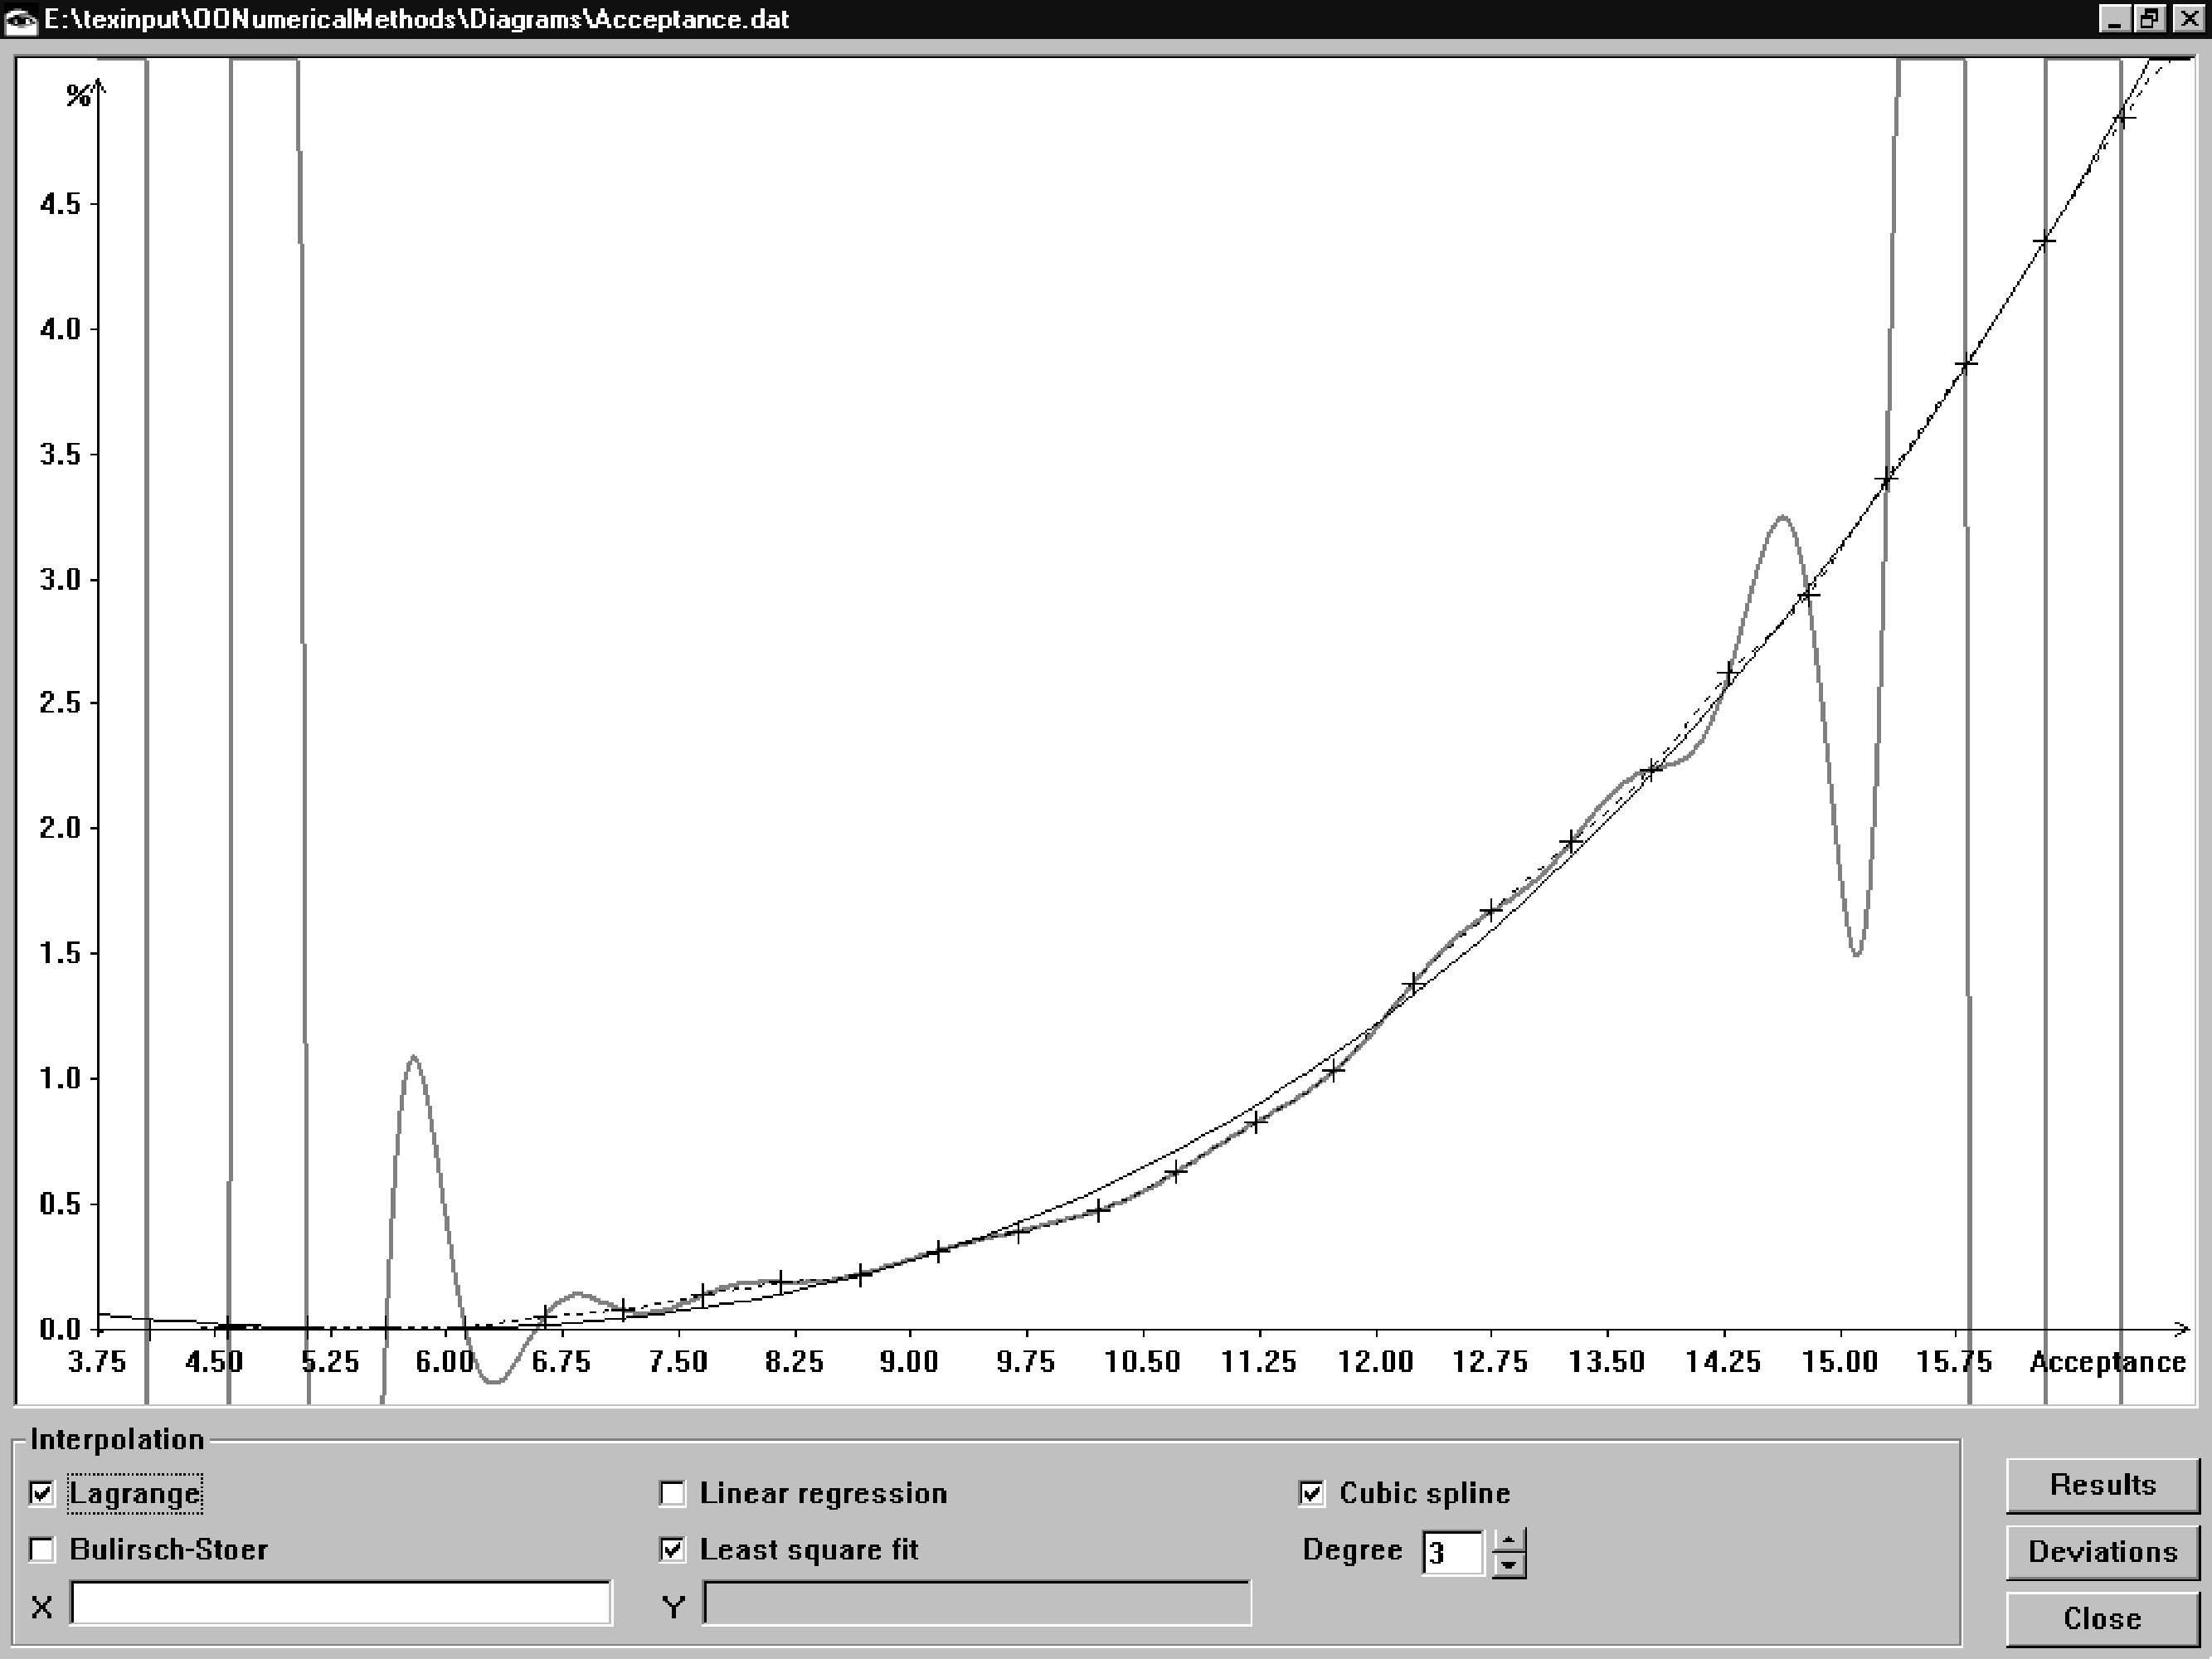
\includegraphics[width=12cm]{Figures/BadInterpolation}
\caption{Example of misbehaving interpolation}
\end{figure}
In this case, however, the simulation was based on using
experimental data. Contrary to the points of figure
\ref{fig:landauinterpol} the points of figure
\ref{fig:interpolex4} are subjected to large fluctuations, because
the sample points have been derived from measured data. Thus,
interpolation does not work.

As in figure \ref{fig:interpolex2}, the gray thick line is the
Lagrange interpolation polynomial and the black dotted line is the
cubic spline. Clearly the Lagrange interpolation polynomial is not
giving any reasonable interpolation. Cubic spline is not really
better as is tries very hard to reproduce the fluctuations of the
computed points. In this case, a polynomial fit (\cf section
\ref{sec:lsfpol}) is the best choice: the thin black line shows
the result of a fit with a $3^{rd}$ degree polynomial.
Another example of unstable interpolation is given in
section \ref{sec:lsfpol} (figure \ref{fig:femurLength}).

\rubrique{Three implementations of Lagrange interpolation} Once
you have verified that a Lagrange interpolation polynomial can be
used to perform reliable interpolation over the sample points, you
must chose among 3 algorithms to compute the Lagrange
interpolation polynomial: direct Lagrange formula, Newton's
algorithm and Neville's algorithm.

Newton's algorithm stores intermediate values which only depends
on the sample points. It is thus recommended, as it is the fastest
method to interpolate several values over the same sample points.
Newton's algorithm is the method of choice to compute a function
from tabulated values.

Neville's algorithm gives an estimate of the numerical error
obtained by the interpolation. It can be used when such
information is needed. Romberg integration, discussed in section
\ref{sec:romberg}, uses Neville's method for that reason.

\section{Lagrange interpolation}
\label{sec:lagrange}
 Let us assume a set of numbers
$x_0,\ldots,x_n$ and the corresponding function's values
$y_0,\ldots,y_n$. There exist a unique polynomial
$P_n\left(x\right)$ of degree $n$ such that
$P_n\left(x_i\right)=y_i$ for all $i=0,\ldots,n$. This polynomial
is the Lagrange interpolation polynomial whose expression is given
by \cite{Knuth2}:
\begin{equation}
\label{eq:lagrange} P_n\left(x\right)=\sum_{i=0}^n{\prod_{j\neq
i}\left(x-x_j\right) \over\prod_{j\neq i}\left(x_i-x_j\right)}y_i.
\end{equation}
For example, the Lagrange interpolation polynomial of degree 2 on
3 points is given by:
\begin{equation}
P_2\left(x\right)={\left(x-x_1\right)\left(x-x_2\right)\over
\left(x_0-x_1\right)\left(x_0-x_2\right)}y_0+{\left(x-x_0\right)\left(x-x_2\right)\over
\left(x_1-x_0\right)\left(x_1-x_2\right)}y_1+{\left(x-x_0\right)\left(x-x_1\right)\over
\left(x_2-x_0\right)\left(x_2-x_1\right)}y_2
\end{equation}

The computation of the polynomial occurs in the order of $\mathcal{O}(n^2)$ since it involves a double iteration.
One can save the evaluation of a few products by rewriting equation \ref{eq:lagrange} as:
\begin{equation}
\label{eq:lagrangesimp}
P_n\left(x\right)=\prod_{i=0}^n\left(x-x_i\right)\sum_{i=0}^n{y_i
\over\left(x-x_i\right)\prod_{j\neq i}\left(x_i-x_j\right)}.
\end{equation}
Of course, equation \ref{eq:lagrangesimp} cannot be evaluated at
the points defining the interpolation. This is easily solved by
returning the defining values as soon as one of the first products
becomes zero during the evaluation.

\subsection{Lagrange interpolation --- Smalltalk implementation}
%\label{sec:slagrange}\marginpar{Figure \ref{cls:interpolation} with the box {\textbf LagrangeInterpolator} grayed.}
The object responsible to implement Lagrange interpolation is defined
uniquely by the sample points over which the interpolation is
performed. In addition it should behave as a function. In other
words it should implement the behavior of a one-variable function
as discussed in section \ref{sec:stFunction}. For example linear
interpolation behaves as follows:

\begin{listing}[label=ex:lagrangeS1]{Smalltalk}
{Linear interpolation}
| interpolator |
interpolator := PMLagrangeInterpolator
                        points: (Array with: 1 @ 2
                                        with: 3 @ 1).
interpolator value: 2.2
\end{listing}

In this example, one creates a new instance of the class \code{PMLagrangeInterpolator} by sending the message \code{points:} to the class \code{PMLagrangeInterpolator} with the collection of
sample points as argument.
The newly created instance is stored in the variable \code{interpolator}.
The next line shows how to compute an interpolated value.

The creation method \code{points:} takes as argument the collection
of sample points. However, it could also accept any object
implementing a subset of the methods of the class \code{Collection}
--- namely the methods \code{size}, \code{at:} and, if we want to be
able to add new sample points, \code{add:}.

One can also spare the creation of an explicit collection object
by implementing these collection methods directly in the Lagrange
interpolation class.
Now, one can also perform interpolation in the following way:

\begin{listing}[label=ex:lagrangeS2]{Smalltalk}
{Alternate way to do a linear interpolation}
| interpolator deviation |
interpolator := PMLagrangeInterpolator new.
1 to: 45 by: 2 do:
                [ :x | interpolator add: x @ (x degreesToRadians sin)].
deviation := (interpolator value: 8) -(8 degreesToRadians sin).
\end{listing}

The code above creates an instance of the class \code{PMLagrangeInterpolator} with an empty collection of sample points. It then adds sample points one by one directly into the
interpolator object. Here the sample points are tabulated values
of the sine function for odd degree values between 1 and 45
degree. The final line of the code compares the interpolated value
with the correct one.

Listing \ref{lst:lagrange} shows the full code of the class
implementing the interface shown above.

The class \code{PMLagrangeInterpolator} is implemented with a
single instance variable containing the collection of sample
points. Each point contains a pair of values
$\left(x_i,y_i\right)$ and is implemented with object of the base
class \code{Point} since an instance of \code{Point} can contain any
type of object in its coordinates. There are two creation methods,
\code{points:} and \code{new}, depending on whether the sample
points are supplied as an explicit object or not. Each creation
method calls in turn an initialization method, respectively \code{initialize:} and \code{initialize}.

The method \code{points:} takes as argument the collection of the
sample points. This object must implement the following methods of
the class \code{Collection}: \code{size}, \code{at:} and \code{add:}.
If the class is created with the method \code{new} an implicit
collection object is created with the method \code{defaultSamplePoints}. This arrangement allows subclasses to select
another type of collection if needed. The default collection
behavior implemented by the class \code{PMLagrangeInterpolator} is
minimal, however. If there is a need for more flexible access to
the collection of sample points, a proper collection object or a
special purpose object should be used.

The interpolation itself is implemented within the single method
\code{value:}. This method is unusually long for object-oriented
programming standards. In this case, however, there is no
compelling reason to split any portion of the algorithm into a
separate method.
Moreover, splitting the method would increase the
computing time.

A final discussion should be made about the two methods \code{xPointAt:} and \code{yPointAt:}.
In principle, there is no need for these methods as the value could be grabbed directly from the collection of points.
If one needs to change the implementation of the point collection in a subclass, however, only these two methods need to be modified.
Introducing this kind of construct can go a long way in program maintenance.

\begin{listing}[label=lst:lagrange]{Smalltalk}
{Smalltalk implementation of the Lagrange interpolation}
Object subclass: #PMLagrangeInterpolator
   instanceVariableNames: 'pointCollection'
   classVariableNames: ''
   package: 'Math-DHB-Numerical-Math-Interpolator'
\end{listing}

\begin{displaycode}{Smalltalk}
PMLagrangeInterpolator class >> new
    ^super new initialize
\end{displaycode}

\begin{displaycode}{Smalltalk}
PMLagrangeInterpolator class >> points: aCollectionOfPoints
    ^self new initialize: aCollectionOfPoints
\end{displaycode}

\begin{displaycode}{Smalltalk}
PMLagrangeInterpolator add: aPoint
    ^pointCollection add: aPoint
\end{displaycode}

\begin{displaycode}{Smalltalk}
PMLagrangeInterpolator >> defaultSamplePoints
    ^OrderedCollection new
\end{displaycode}

\begin{displaycode}{Smalltalk}
PMLagrangeInterpolator >> initialize
    ^self initialize: self defaultSamplePoints
\end{displaycode}

\begin{displaycode}{Smalltalk}
PMLagrangeInterpolator >> initialize: aCollectionOfPoints
    pointCollection := aCollectionOfPoints.
    ^self
\end{displaycode}

\begin{displaycode}{Smalltalk}
PMLagrangeInterpolator >> value: aNumber
    | norm dx products answer size |
    norm := 1.
    size := pointCollection size.
    products := Array new: size.
    products atAllPut: 1.
    1 to: size
        do: [ :n |
              dx := aNumber - ( self xPointAt: n).
              dx = 0
                ifTrue: [ ^( self yPointAt: n)].
              norm := norm * dx.
              1 to: size
                do: [ :m |
                      m = n
                        ifFalse:[ products at: m put: ( (( self 
            xPointAt: m) - ( self xPointAt: n)) * ( products at: m))].
                    ].
            ].
    answer := 0.
    1 to: size do:
        [ :n | answer := ( self yPointAt: n) / ( ( products at: n) * 
                          ( aNumber - ( self xPointAt: n))) + answer].
    ^norm * answer
\end{displaycode}

\begin{displaycode}{Smalltalk}
PMLagrangeInterpolator >> xPointAt: anInteger
    ^( pointCollection at: anInteger) x
\end{displaycode}

\begin{displaycode}{Smalltalk}
PMLagrangeInterpolator >> yPointAt: anInteger
    ^( pointCollection at: anInteger) y
\end{displaycode}

\section{Newton interpolation}
\label{sec:newtoninterpol} If one must evaluate the Lagrange
interpolation polynomial for several values, it is clear that the
Lagrange's formula is not efficient. Indeed a portion of the terms
in the summation of equation \ref{eq:lagrangesimp} depends only on
the sample points and does not depend on the value at which the
polynomial is evaluated. Thus, one can speed up the evaluation of
the polynomial if the invariant parts are computed once and
stored.

If one writes the Lagrange interpolation polynomial using a
generalized Horner expansion, one obtains the Newton's
interpolation formula given by \cite{Knuth2}:
\begin{equation}
\label{eq:newtonhorn}P_n\left(x\right)=\alpha_0+\left(x-x_0\right)\cdot
\left[\alpha_1+\left(x-x_1\right)\cdot\left[\cdots\left[\alpha_{n-1}+\alpha_n\cdot\left(x-x_1\right)\right]\right]\right]
\end{equation}
The coefficients $\alpha_i$ are obtained by evaluating divided
differences as follows:
\begin{equation}
\label{eq:newtoncoef}\left\{ \begin{array}{lcl}\Delta_i^0 &=&y_i
\\ \Delta_i^k &=&{\Delta_i^{k-1}-\Delta_{i-1}^{k-1}\over
x_i-x_{i-k}}\mbox{\quad for $k=1,\ldots,n$}
\\ \alpha_i &=&\Delta_i^i
\end{array}\right.
\end{equation}
Once the coefficients $\alpha_i$ have been obtained, they can be
stored in the object and the generalized Horner expansion of
equation \ref{eq:newtonhorn} can be used.

The time to evaluate the full Newton's algorithm --- that is
computing the coefficients and evaluating the generalized Horner
expansion --- is about twice the time needed to perform a direct
Lagrange interpolation. The evaluation of the generalized Horner
expansion alone, however, has an execution time of $\mathcal{O}(n)$ and
is therefore much faster than the evaluation of a direct Lagrange
interpolation which goes as $\mathcal{O}(n^2)$. Thus, as soon as one needs
to interpolate more than 2 points over the same point sample,
Newton's algorithm is more efficient than direct Lagrange
interpolation.

\subsection{Newton interpolation --- Smalltalk implementation}
%\marginpar{Figure \ref{cls:interpolation} with the box {\textbf NewtonInterpolator} grayed.}
The object implementing Newton's interpolation algorithm is best implemented as a subclass of the
class \code{PMLagrangeInterpolator} because all methods used to
handle the sample points can be reused. This also allows us to
keep the interface identical. It has an additional instance
variable needed to store the coefficients $\alpha_i$. Only 4 new
methods are needed.

Since the client object can add new sample points at will, one
cannot be sure of when it is safe to compute the coefficients.
Thus, computing the coefficients is done with lazy initialization.
The method \code{value:} first checks whether the coefficients
$\alpha_i$ have been computed. If not, the method \code{computeCoefficients} is called. Lazy initialization is a technique
widely used in object oriented programming whenever some value
needs only be computed once.

\noindent The generalized Horner expansion is implemented in the
method \code{value:}.

If a new sample point is added, the coefficient eventually stored
in the object are no longer valid. Thus, the method \code{add:}
first calls the method \code{resetCoefficients} and then calls the
method \code{add:} of the superclass. The method \code{resetCoefficients} makes sure that the coefficients will be
computed anew at the next evaluation of the interpolation
polynomial. The method \code{resetCoefficients} has been
implemented as a separate method so that the reset mechanism can
be reused by any subclass.

Another reason to keep the method \code{resetCoefficients} separate
is that it must also be called before doing an interpolation if
the sample points have been modified directly by the client
application after the last interpolation has been made. An
alternative is to implement the \patstyle{Observable/Observer}
pattern so that resetting of the coefficients happens implicitly
using events. However, since modifying the sample points between
interpolation should only be a rare occasion when using Newton's
algorithm\footnote{If modification of the sample points is not a
rare occasion, then Newton's algorithm has no advantage over
direct Lagrange interpolation or Neville's algorithm. Those
algorithms should be used instead of Newton's algorithm.} our
proposed implementation is much simpler.

Listing \ref{lst:newtonint} shows the complete implementation in
Smalltalk. The class \code{NewtonInterpolator} is a subclass of
class \code{LagrangeInterpolator}. The code examples
\ref{ex:lagrangeS1} and \ref{ex:lagrangeS2} can directly be
applied to Newton interpolation after replacing the class name \code{PMLagrangeInterpolator} with \code{PMNewtonInterpolator}.

The generalized Horner expansion is implemented in the method \code{value:} using explicit indices. One could have used the method \code{inject:into:} as it was done for Horner's formula when
evaluating polynomials. In this case, however, one must still keep
track of the index to retrieve the sample point corresponding to
each coefficient. Thus, one gains very little in compactness.

\begin{listing}[label=lst:newtonint]{Smalltalk}
{Smalltalk implementation of the Newton interpolation}
PMLagrangeInterpolator subclass: #PMNewtonInterpolator
   instanceVariableNames: 'coefficients'
   classVariableNames: ''
   package: 'Math-DHB-Numerical-Math-Interpolator'
\end{listing}

\begin{displaycode}{Smalltalk}
PMNewtonInterpolator >> add: aPoint
    self resetCoefficients.
    ^super add: aPoint
\end{displaycode}

\begin{displaycode}{Smalltalk}
PMNewtonInterpolator >> computeCoefficients
    | size k1 kn|
    size := pointCollection size.
    coefficients := ( 1 to: size) collect: [ :n | self yPointAt: n].
    1 to: (size - 1)
        do: [ :n |
              size to: ( n + 1)  by: -1
                do: [ :k |
                      k1 := k - 1.
                      kn := k - n.
                      coefficients at: k put: ( (( coefficients at: 
                                         k) - ( coefficients at: k1)) 
                                            / ((self xPointAt: k) - 
                                                (self xPointAt: kn))).
                    ].
            ].
\end{displaycode}

\begin{displaycode}{Smalltalk}
PMNewtonInterpolator >> resetCoefficients
    coefficients := nil.
\end{displaycode}

\begin{displaycode}{Smalltalk}
PMNewtonInterpolator >> value: aNumber
    | answer size |
    coefficients isNil
        ifTrue: [ self computeCoefficients].
    size := coefficients size.
    answer := coefficients at: size.
    (size - 1) to: 1 by: -1
        do: [ :n | answer := answer * ( aNumber - (self xPointAt:  
                                         n)) + ( coefficients at: n)].
    ^answer
\end{displaycode}

\section{Neville interpolation}
\label{sec:neville} Neville's algorithm uses a successive
approximation approach implemented in practice by calculating
divided differences recursively. The idea behind the algorithm is
to compute the value of the interpolation's polynomials of all
degrees between 0 and $n$. This algorithm assumes that the sample
points have been sorted in increasing order of abscissa.

Let $P^i_j\left(x\right)$ be the (partial) Lagrange interpolation
polynomials of degree $i$ defined by the sets of values
$x_j,\ldots,x_{j+i}$ and the corresponding function's values
$y_j,\ldots,y_{j+i}$. From equation \ref{eq:lagrange} one can
derive the following recurrence formula \cite{Press}:
\begin{equation}
\label{eq:neville}
P^i_j\left(x\right)={\left(x-x_{i+j}\right)P^{i-1}_j\left(x\right)
+\left(x_j-x\right)P^{i-1}_{j+1}\left(x\right)\over x_j-x_{i+j}}
\mbox{\quad for $j<i$}.
\end{equation}
The initial values $P^0_j\left(x\right)$ are simply $y_j$. The
value of the final Lagrange's polynomial is $P^n_0\left(x\right)$.

Neville's algorithm introduces the differences between the
polynomials of various degrees. One defines:
\begin{equation}
\left\{ \begin{array}{lcl} \Delta_{j,i}^{\mathop
{left}}\left(x\right)
&=&P^i_j\left(x\right)-P^{i-1}_j\left(x\right)
\\*[3 ex] \Delta_{j,i}^{\mathop{right}}\left(x\right) &=&P^i_j\left(x\right)-P^{i-1}_{j+1}\left(x\right)
\end{array}\right.
\end{equation}
From the definition above and equation \ref{eq:neville} one
derives a pair of recurrence formulae for the differences:
\begin{equation}
\left\{ \begin{array}{lcl}\Delta_{j,i+1}^{\mathop
{left}}\left(x\right) &=&{x_i-x\over
x_j-x_{i+j+1}}\left(\Delta_{j+1,i}^{\mathop
{left}}\left(x\right)-\Delta_{j,i}^{\mathop
{right}}\left(x\right)\right)
\\*[3 ex] \Delta_{j,i+1}^{\mathop{right}} &=&{x_{i+j+1}-x\over
x_j-x_{i+j+1}}\left(\Delta_{j+1,i}^{\mathop
{left}}\left(x\right)-\Delta_{j,i}^{\mathop
{right}}\left(x\right)\right)
\end{array}\right.
\end{equation}
In practice two arrays of differences --- one for left and one for
right --- are allocated. Computation of each order is made within
the same arrays. The differences of the last order can be
interpreted as an estimation of the error made in replacing the
function by the interpolation's polynomial.

Neville's algorithm is faster than the evaluation of direct
Lagrange's interpolation for a small number of points (smaller
than about 7\footnote{\cf footnote \ref{ft:lagnev} on page
\pageref{ft:lagnev}}. Therefore a simple linear interpolation is
best performed using Neville's algorithm. For a large number of
points, it becomes significantly slower.

\subsection{ Neville interpolation --- Smalltalk  implementation}
%\marginpar{Figure \ref{cls:interpolation} with the box {\textbf NevilleInterpolator} grayed.}
The object implementing Neville's interpolation's algorithm is best implemented as a subclass of the
class \code{LagrangeInterpolator} since the methods used to handle
the sample points can be reused. This also allows us to keep the
interface identical.

The new class has two additional instance variables used to store
the finite differences $\Delta_{j,i}^{\mathop{
left}}\left(x\right)$ and $\Delta_{j,i}^{\mathop{
right}}\left(x\right)$ for all $j$.
These instance variables are recycled for all $i$.
Only a few additional methods are needed.

The method \code{valueAndError:} implementing Neville's algorithm
returns an array with two elements: the first element is the
interpolated value and the second is the estimated error. The
method \code{value:} calls the former method and returns only the
interpolated value.

Unlike other interpolation algorithms, the method \code{valueAndError:} is broken into smaller methods because the
mechanics of computing the finite differences will be reused in
the Bulirsch-Stoer algorithm. The method \code{valueAndError:}
begins by calling the method \code{initializeDifferences:} to
populate the arrays containing the finite differences with their
initial values. These arrays are created if this is the first time
they are used with the current sample points. This prevents
unnecessary memory allocation. Then, at each iteration the method \code{computeDifference:at:order:} computes the differences for the current order.

Listing \ref{lst:neville} shows the implementation of Neville's
algorithm in Smalltalk. The class \code{PMNevilleInterpolator} is
a subclass of class \code{PMLagrangeInterpolator}. The code
examples \ref{ex:lagrangeS1} and \ref{ex:lagrangeS2} can directly
be applied to Neville interpolation after replacing the class name
\code{PMLagrangeInterpolator} with \code{PMNevilleInterpolator}.
An example of interpolation using the returned estimated error is
given in section \ref{sec:sromberg}.

The method \code{defaultSamplePoints} overrides that of the
superclass to return a sorted collection. Thus, each point added
to the implicit collection is automatically sorted by increasing
abscissa as required by Neville's algorithm.

\begin{listing}[label=lst:neville]{Smalltalk}
{Smalltalk implementation of Neville's algorithm}
PMLagrangeInterpolator subclass: #PMNevilleInterpolator
   instanceVariableNames: 'leftErrors rightErrors'
   classVariableNames: ''
   package: 'Math-DHB-Numerical-Math-Interpolator'
\end{listing}

\begin{displaycode}{Smalltalk}
PMNevilleInterpolator >> computeDifference: aNumber at: anInteger1 order: anInteger2
    | leftDist rightDist ratio |
    leftDist := ( self xPointAt: anInteger1) - aNumber.
    rightDist := (  self xPointAt: ( anInteger1 + anInteger2)) - 
                                                              aNumber.
    ratio := ( ( leftErrors at: ( anInteger1 + 1)) - ( rightErrors 
                           at: anInteger1)) / ( leftDist - rightDist).
    leftErrors at: anInteger1 put: ratio * leftDist.
    rightErrors at: anInteger1 put: ratio * rightDist.
\end{displaycode}

\begin{displaycode}{Smalltalk}
PMNevilleInterpolator >> defaultSamplePoints
    ^SortedCollection sortBlock: [ :a :b | a x < b x]
\end{displaycode}

\begin{displaycode}{Smalltalk}
PMNevilleInterpolator >> initializeDifferences: aNumber
    | size nearestIndex dist minDist |
    size := pointCollection size.
    leftErrors size = size
        ifFalse:[ leftErrors := Array new: size.
                  rightErrors := Array new: size.
                ].
    minDist := ( ( self xPointAt: 1) - aNumber) abs.
    nearestIndex := 1.
    leftErrors at: 1 put: ( self yPointAt: 1).
    rightErrors at: 1 put: leftErrors first.
    2 to: size do:
        [ :n |
          dist := ( ( self xPointAt: n) - aNumber) abs.
          dist < minDist
            ifTrue: [ dist = 0
                        ifTrue: [ ^n negated].
                      nearestIndex := n.
                      minDist := dist.
                    ].
         leftErrors at: n put: ( self yPointAt: n).
         rightErrors at: n put: ( leftErrors at: n).
        ].
    ^nearestIndex
\end{displaycode}

\begin{displaycode}{Smalltalk}
PMNevilleInterpolator >> value: aNumber
    ^(self valueAndError: aNumber) first
\end{displaycode}

\begin{displaycode}{Smalltalk}
PMNevilleInterpolator >>valueAndError: aNumber
    | size nearestIndex answer error |
    nearestIndex := self initializeDifferences: aNumber.
    nearestIndex < 0
        ifTrue: [ ^Array with: ( self yPointAt: nearestIndex negated) 
                                                             with: 0].
    answer := leftErrors at: nearestIndex.
    nearestIndex := nearestIndex - 1.
    size := pointCollection size.
    1 to: ( size - 1) do:
        [ :m |
          1 to: ( size - m) do:
            [ :n | self computeDifference: aNumber at: n order: m].
          size - m > ( 2 * nearestIndex)
                ifTrue: [ error := leftErrors at: ( nearestIndex + 1) 
                                                                     ]
                ifFalse:[ error := rightErrors at: ( nearestIndex).
                              nearestIndex := nearestIndex - 1.
                            ].
          answer := answer + error.
        ].
    ^Array with: answer with: error abs

\end{displaycode}

\section{Bulirsch-Stoer interpolation}
If the function to interpolate is known to have
poles\footnote{That is, a singularity in the complex plane.} in
the vicinity of the real axis over the range of the sample points
a polynomial cannot do a good interpolation job \cite{Press}.

In this case it is better to use rational function, that is a
quotient of two polynomials as defined hereafter:
\begin{equation}
R\left(x\right)={P\left(x\right)\over Q\left(x\right)}
\end{equation}
The coefficients of both polynomials are only defined up to a
common factor. Thus, if $p$ is the degree of polynomial
$P\left(x\right)$ and $q$ is the degree of polynomial
$Q\left(x\right)$, we must have the relation $p+q+1 = n$ where $n$
is the number of sample points. This of course is not enough to
restrict the variety of possible rational functions.

Bulirsch and Stoer have proposed an algorithm for a rational
function where $p=\lfloor{n-1 \over 2}\rfloor$. This means that
$q$ is either equal to $p$ if the number of sample points is odd
or equal to $p+1$ if the number of sample points is even. Such a
rational function is called a diagonal rational function. This
restriction, of course, limits the type of function shapes that
can be interpolated.

The Bulirsch-Stoer algorithm is constructed like Neville's
algorithm: finite differences are constructed until all points
have been taken into account.

Let $R_j^i\left(x\right)$ be the (partial) diagonal rational
functions of order $i$ defined by the sets of values
$x_j,\ldots,x_{j+i}$ and the corresponding function's values
$y_j,\ldots,y_{j+i}$. As in the case of Neville's algorithm, one
can establish a recurrence formula between functions of successive
orders. We have \cite{Press}:
\begin{equation}
\label{eq:bustoer}
R_j^i\left(x\right)=R_{j+1}^{i-1}\left(x\right)+
{R_{j+1}^{i-1}\left(x\right) - R_j^{i-1}\left(x\right) \over
{x-x_j\over x-x_{i+j}}\left(1-{R_{j+1}^{i-1}\left(x\right)
-R_j^{i-1}\left(x\right)\over R_{j+1}^{i-1}\left(x\right)
-R_{j+1}^{i-2}\left(x\right)}\right)}\mbox{\quad for $j<i$}.
\end{equation}
The initial values $R_j^0\left(x\right)$ are simply $y_j$. The
final rational function is $R_0^n\left(x\right)$.

Like in Neville's algorithm one introduces the differences between
the functions of various orders. One defines:
\begin{equation}
\left\{
\begin{array}{lcl}
    \Delta_{j,i}^{\mathop{\textrm
left}}\left(x\right) & = & R_j^i\left(x\right) -
R_j^{i-1}\left(x\right)\\*[2ex]
    \Delta_{j,i}^{\mathop{\textrm
right}}\left(x\right) & = & R_j^j\left(x\right) -
R_{j+1}^{i-1}\left(x\right)
  \end{array}\right.
\end{equation}
From the definition above and equation \ref{eq:bustoer} one
derives a pair of recurrence formulae for the differences:
\begin{equation}
\left\{
\begin{array}{lcl}
    \Delta_{j,i+1}^{\mathop{\textrm
left}}\left(x\right) & = &{{x-x_j \over x - x_{i+j+1}}
\Delta_{j,i}^{\mathop{\textrm right}}\left(x\right)
\left[\Delta_{j+1,i}^{\mathop{\textrm left}}\left(x\right) -
\Delta_{j,i}^{\mathop{\textrm right}}\left(x\right)\right] \over
{x-x_j \over x-x_{i+j+1}} \Delta_{j,i}^{\mathop{\textrm
right}}\left(x\right) - \Delta_{j+1,i}^{\mathop{\textrm
left}}\left(x\right)}
\\*[3ex]
    \Delta_{j,i}^{\mathop{\textrm
right}}\left(x\right) & = &{ \Delta_{j+1,i}^{\mathop{\textrm
left}}\left(x\right) \left[\Delta_{j+1,i}^{\mathop{\textrm
left}}\left(x\right) - \Delta_{j,i}^{\mathop{\textrm
right}}\left(x\right)\right] \over {x-x_j \over x-x_{i+j+1}}
\Delta_{j,i}^{\mathop{\textrm right}}\left(x\right) -
\Delta_{j+1,i}^{\mathop{\textrm left}}\left(x\right)}
  \end{array}\right.
\end{equation}
Like for Neville's algorithm, two arrays of differences --- one
for left and one for right --- are allocated. Computation of each
order is made within the same arrays. The differences of the last
order can be interpreted as an estimation of the error made in
replacing the function by the interpolating rational function.
Given the many similarities with Neville's algorithm many methods
of that algorithm can be reused.

\subsection{Bulirsch-Stoer interpolation --- Smalltalk implementation}

%\marginpar{Figure \ref{cls:interpolation} with the box {\textbf BulirschStoerInterpolator} grayed.}
The object implementing Bulirsch-Stoer interpolation's algorithm is best implemented as a
subclass of the class \code{PMNevilleInterpolator} since the
methods used to manage the computation of the finite differences
can be reused. The public interface is identical.

Only a single method --- the one responsible for the evaluation of
the finite differences at each order --- must be implemented. All
other methods of Neville's interpolation can be reused.

This shows the great power of object-oriented approach. Code
written in procedural language cannot be reused that easily. In
\cite{Press} the two codes implementing Neville's and
Bulirsch-Stoer interpolation are of comparable length; not
surprisingly they also have much in common.

Listing \ref{lst:bustoer} shows the implementation of
Bulirsch-Stoer interpolation in Smalltalk. The class \code{PMBulirschStoerInterpolator} is a subclass of class \code{PMNevilleInterpolator}. The code examples \ref{ex:lagrangeS1} and
\ref{ex:lagrangeS2} can directly be applied to Bulirsch-Stoer
interpolation after replacing the class name \code{PMLagrangeInterpolator} with \code{PMBulirschStoerInterpolator}.

\begin{listing}[label=lst:bustoer]{Smalltalk}
{Smalltalk implementation of Bulirsch-Stoer interpolation}
PMNevilleInterpolator subclass: #PMBulirschStoerInterpolator
   instanceVariableNames: ''
   classVariableNames: ''
   package: 'Math-DHB-Numerical-Math-Interpolator'
\end{listing}

\begin{displaycode}{Smalltalk}
PMBulirschStoerInterpolator >> computeDifference: aNumber at: anInteger1 order: anInteger2
    | diff ratio |
    ratio := ( ( self xPointAt: anInteger1) - aNumber) * ( 
                                           rightErrors at: anInteger1)
                            / ( (  self xPointAt: ( anInteger1 + 
                                              anInteger2)) - aNumber).
    diff := ( ( leftErrors at: ( anInteger1 + 1)) - ( rightErrors at: 
                                                          anInteger1))
                            / ( ratio - ( leftErrors at: ( anInteger1 
                                                               + 1))).
    rightErrors at: anInteger1 put: ( leftErrors at: ( anInteger1 + 
                                                          1)) * diff. 
    leftErrors at: anInteger1 put: ratio * diff.
\end{displaycode}

\section{Cubic spline interpolation}
The Lagrange interpolation polynomial is defined globally over the
set of given points and respective function's values. As we have
seen in figure \ref{fig:interpolex4} and to a lesser degree in
figure \ref{fig:interpolex3} Lagrange's interpolation polynomial
can have large fluctuations between two adjacent points because
the degree of the interpolating polynomial is not constrained.

One practical method for interpolating a set of function's value
with a polynomial of constrained degree is to use cubic splines. A
cubic spline is a $3^{\mathop{\textrm rd}}$ order polynomial
constrained in its derivatives at the end points. A unique cubic
spline is defined for each interval between two adjacent points.
The interpolated function is required to be continuous up to the
second derivative at each of the points.

Before the advent of computers, people were drawing smooth curves
by sticking nails at the location of computed points and placing
flat bands of metal between the nails. The bands were then used as
rulers to draw the desired curve. These bands of metal were called
splines and this is where the name of the interpolation algorithm
comes from. The elasticity property of the splines correspond to
the continuity property of the cubic spline function.

The algorithm exposed hereafter assumes that the sample points
have been sorted in increasing order of abscissa.

To derive the expression for the cubic spline, one first assumes
that the second derivatives of the splines, $y^{\prime\prime}_i$,
are known at each point. Then one writes the cubic spline between
$x_{i-1}$ and $x_i$ in the following symmetric form:
\begin{equation}
\label{eq:splinedef} P_i\left(x\right)=y_{i-1}A_i\left(x\right) +
y_i B_i\left(x\right) + y^{\prime\prime}_{i-1}C_i\left(x\right) +
y^{\prime\prime}_i D_i\left(x\right),
\end{equation}
where
\begin{equation}
\label{eq:splinelin}  \left\{
  \begin{array}{lcl}
    A_i\left(x\right) & = & \displaystyle x_i - x \over\displaystyle x_i - x_{i-1}, \\*[2 ex]
    B_i\left(x\right) & = & \displaystyle x - x_{i-1} \over\displaystyle x_i - x_{i-1}.
  \end{array}\right.
\end{equation}
Using the definition above, the first two terms in equation
\ref{eq:splinedef} represents the linear interpolation between the
two points $x_{i-1}$ and $x_i$. Thus, the last two terms of must
vanish at $x_{i-1}$ and $x_i$. In addition we must have by
definition:
\begin{equation}
\label{eq:splinedifeq}
 \left\{
  \begin{array}{lcl}
    \left.{\displaystyle d^2P_i\left(x\right)\over\displaystyle dx^2}\right|_{x=x_{i-1}} & = &
    y^{\prime\prime}_{i-1},
    \\*[3 ex]
    \left.{\displaystyle d^2P_i\left(x\right)\over\displaystyle dx^2}\right|_{x=x_i} & = &
    y^{\prime\prime}_i.
  \end{array} \right.
\end{equation}
One can rewrite the first equation in \ref{eq:splinedifeq} as a
differential equation for the function $C_i$ as a function of
$A_i$. Similarly, the second equation is rewritten as a
differential equation for the function $D_i$ as a function of
$B_i$. This yields:
\begin{equation}
\label{eq:splinecub}
 \left\{
  \begin{array}{lcl}
    C_i\left(x\right) & = &
    {\displaystyle A_i\left(x\right)\left[A_i\left(x\right)^2-1\right]\over\displaystyle 6} \left(x_i - x_{i-1}\right)^2,
    \\*[3 ex]
    D_i\left(x\right) & = &
    {\displaystyle B_i\left(x\right)\left[B_i\left(x\right)^2-1\right]\over\displaystyle 6} \left(x_i - x_{i-1}\right)^2,
  \end{array} \right.
\end{equation}
Finally, one must use the fact that the first derivatives of each
spline must be equal at each end points of the interval, that is:
\begin{equation}
 {dP_i\left(x\right)\over dx}={dP_{i+1}\left(x\right)\over dx}.
\end{equation}
This yields the following equations for the second derivatives
$y^{\prime\prime}_i$:
\begin{equation}
\label{eq:splinesyst}
  {x_{i+1}-x_i \over 6}y^{\prime\prime}_{i+1}
  + {x_{i+1}-x_{i-1} \over  6}y^{\prime\prime}_i
  + {x_i-x_{i-1} \over 6}y^{\prime\prime}_{i-1}=
  {y_{i+1}-y_i \over x_{i+1}-x_i} - {y_i-y_{i-1} \over  x_i-x_{i-1}}.
\end{equation}
There are $n-1$ equations for the $n$ unknowns
$y^{\prime\prime}_i$. We are thus missing two equations. There are
two ways of defining two additional equations to obtain a unique
solution.
\begin{itemize}
  \item The first method is the so-called natural cubic spline for which
one sets $y^{\prime\prime}_0=y^{\prime\prime}_n=0$. This means
that the spline is flat at the end points.
  \item The second method is called constrained cubic spline. In this case the
first derivatives of the function at $x_0$ and $x_n$,
$y^{\prime}_0$ and $y^{\prime}_n$, are set to given values.
\end{itemize}

In the case of constrained cubic spline, one obtain two additional
equations by evaluating the derivatives of equation
\ref{eq:splinedef} at $x_0$ and $x_n$:
\begin{equation}
\label{eq:splineend}
 \left\{
  \begin{array}{lcl}
    {3A_1\left(x\right)^2-1\over 6}\left(x_1-x_0\right) y^{\prime\prime}_0 -
    {3B_1\left(x\right)^2-1\over 6}\left(x_1-x_0\right) y^{\prime\prime}_1 & = &
    y^{\prime}_0 - {y_1-y_0 \over x_1-x_0},
    \\*[3 ex]
    {3A_n\left(x\right)^2-1\over 6}\left(x_n-x_{n-1}\right) y^{\prime\prime}_n -
    {3B_n\left(x\right)^2-1\over 6}\left(x_n-x_{n-1}\right) y^{\prime\prime}_{n-1} & = &
    y^{\prime}_n - {y_n-y_{n-1} \over x_n-x_{n-1}}.
  \end{array} \right.
\end{equation}
The choice between natural or constrained spline can be made
independently at each end point.

One solves the system of equations \ref{eq:splinesyst}, and
possibly \ref{eq:splineend}, using direct Gaussian elimination and
back substitution (\cf section \ref{sec:lineqs}). Because the
corresponding matrix is tridiagonal, each pivoting step only
involves one operation. Thus, resorting to a general algorithm for
solving a system of linear equations is not necessary.

\subsection{Cubic spline interpolation --- Smalltalk  implementation}
%\marginpar{Figure \ref{cls:interpolation} with the box {\textbf SplineInterpolator} grayed.}
In both languages the object implementing cubic spline interpolation is a subclass of the
Newton interpolator. The reader might be surprised by this choice
since, mathematically speaking, these two objects do not have
anything in common.

However, from the behavioral point of view, they are quite
similar. Like for Newton interpolation, cubic spline interpolation
first needs to compute a series of coefficients, namely the second
derivatives, which only depends on the sample points. This
calculation only needs to be performed once. Then the evaluation
of the function can be done using equations \ref{eq:splinedef},
\ref{eq:splinelin} and \ref{eq:splinecub}. Finally, as for the
Newton interpolator, any modification of the points requires a new
computation of the coefficients. The behavior can be reused from
the class \code{NewtonInterpolator}.

The second derivatives needed by the algorithm are stored in the
variable used to store the coefficients of Newton's algorithm.

The class \code{SplineInterpolator} has two additional instance
variables needed to store the end point derivatives $y^{\prime}_0$
and $y^{\prime}_n$. Corresponding methods needed to set or reset
these values are implemented. If the value of $y^{\prime}_0$ or
$y^{\prime}_n$ is changed then the coefficients must be reset.

Natural or constrained cubic spline is flagged independently at
each point by testing if the corresponding end-point derivative
has been supplied or not. The second derivatives are computed used
lazy initialization by the method \code{computeSecondDerivatives}.

Listing \ref{lst:spline} shows the implementation of cubic spline
interpolation in Smalltalk. The class \code{PMSplineInterpolator}
is a subclass of class \code{PMNewtonInterpolator}. The code
examples \ref{ex:lagrangeS1} and \ref{ex:lagrangeS2} can directly
be applied to cubic spline interpolation after replacing the class
name \code{PMLagrangeInterpolator} with \code{PMSplineInterpolator}.

If the end-point derivative is \code{nil} the corresponding
end-point is treated as a natural spline.

The method \code{defaultSamplePoints} overrides that of the
superclass to create a sorted collection. Thus, as each point is
added to the implicit collection, the collection of sample points
remains in increasing order of abscissa as required by the cubic
spline algorithm.

\begin{listing}[label=lst:spline]{Smalltalk}
{Smalltalk implementation of cubic spline interpolation}
PMNewtonInterpolator subclass: #PMSplineInterpolator
   instanceVariableNames: 'startPointDerivative endPointDerivative'
   classVariableNames: ''
   package: 'Math-DHB-Numerical-Math-Interpolator'
\end{listing}

\begin{displaycode}{Smalltalk}
PMSplineInterpolator >> computeSecondDerivatives
    | size u w s dx inv2dx |
    size := pointCollection size.
    coefficients := Array new: size.
    u := Array new: size - 1.
    startPointDerivative isNil 
        ifTrue: 
            [coefficients at: 1 put: 0.
            u at: 1 put: 0]
        ifFalse: 
            [coefficients at: 1 put: -1 / 2.
            s := 1 / (( self xPointAt: 2) x - ( self xPointAt: 1) x).
            u at: 1
                put: 3 * s 
                        * (s * (( self yPointAt: size) - ( self 
                                                 yPointAt: size - 1)) 
                                - startPointDerivative)].
    2 to: size - 1
        do: 
            [:n | 
            dx := (self xPointAt: n) - (self xPointAt: ( n - 1)).
            inv2dx := 1 / (( self xPointAt: n + 1) - (self xPointAt: 
                                                              n - 1)).
            s := dx * inv2dx.
            w := 1 / (s * (coefficients at: n - 1) + 2).
            coefficients at: n put: (s - 1) * w.
            u at: n
                put: (((( self yPointAt: n + 1) - ( self yPointAt: 
                                                                  n)) 
                        / (( self xPointAt: n + 1) - ( self xPointAt: 
                                                                  n)) 
                            - ((( self yPointAt: n) - ( self 
                                         yPointAt: n - 1)) / dx)) * 6 
                        * inv2dx - ((u at: n - 1) * s)) 
                        * w].
    endPointDerivative isNil 
        ifTrue: [coefficients at: size put: 0]
        ifFalse: 
            [w := 1 / 2.
            s := 1 / ((self xPointAt:  size) - (self xPointAt: ( size 
                                                               - 1))).
            u at: 1
                put: 3 * s * (endPointDerivative 
                                - (s * (self yPointAt: size) - (self 
                                                yPointAt: size - 1))).
            coefficients at: size
                put: s - (w * (u at: size - 1) / ((coefficients at: 
                                                 size - 1) * w + 1))].
    size - 1 to: 1
        by: -1
        do: 
            [:n | 
            coefficients at: n
                put: (coefficients at: n) * (coefficients at: n + 1) 
                                                          + (u at: n)]

\end{displaycode}

\begin{displaycode}{Smalltalk}
PMSplineInterpolator >> defaultSamplePoints
    ^SortedCollection sortBlock: [ :a :b | a x < b x]
\end{displaycode}

\begin{displaycode}{Smalltalk}
PMSplineInterpolator >> endPointDerivative: aNumber
    endPointDerivative := aNumber.
    self resetCoefficients
\end{displaycode}

\begin{displaycode}{Smalltalk}
PMSplineInterpolator >> resetEndPointDerivatives
    self setEndPointDerivatives: ( Array new: 2)
\end{displaycode}

\begin{displaycode}{Smalltalk}
PMSplineInterpolator >> setEndPointDerivatives: anArray
    startPointDerivative := anArray at: 1.
    endPointDerivative := anArray at: 2.
    self resetCoefficients
\end{displaycode}

\begin{displaycode}{Smalltalk}
PMSplineInterpolator >> startPointDerivative: aNumber
    startPointDerivative := aNumber.
    self resetCoefficients
\end{displaycode}

\begin{displaycode}{Smalltalk}
PMSplineInterpolator >> value: aNumber
    | answer n1 n2 n step a b |
    coefficients isNil ifTrue: [self computeSecondDerivatives].
    n2 := pointCollection size.
    n1 := 1.
    [n2 - n1 > 1] whileTrue: 
            [n := (n1 + n2) // 2.
            (self xPointAt:  n) > aNumber ifTrue: [n2 := n] ifFalse: 
                                                           [n1 := n]].
    step := (self xPointAt: n2) - (self xPointAt: n1).
    a := ((self xPointAt: n2) - aNumber) / step.
    b := (aNumber - (self xPointAt: n1)) / step.
    ^a * (self yPointAt: n1) + (b * (self yPointAt: n2)) 
        + ((a * (a squared - 1) * (coefficients at: n1) 
                + (b * (b squared - 1) * (coefficients at: n2))) * 
                                                         step squared 
                / 6)
\end{displaycode}

\section{Which method to choose?}
At this point some reader might experience some difficulty in
choosing among the many interpolation algorithms discussed in this
book. There are indeed many ways to skin a cat. Selecting a method
depends on what the user intends to do with the data.

First of all, the reader should be reminded that Lagrange
interpolation, Newton interpolation and Neville's algorithm are
different algorithms computing the values of the same function,
namely the Lagrange interpolation polynomial. In other words, the
interpolated value resulting from each 3 algorithms is the same
(up to rounding errors of course).

The Lagrange interpolation polynomial can be subject to strong
variations (if not wild in some cases, figure
\ref{fig:interpolex4} for example) if the sampling points are not
smooth enough. A cubic spline may depart from the desired function
if the derivatives on the end points are not constrained to proper
values. A rational function can do a good job in cases where
polynomials have problems. To conclude, let me give you some rules
of thumb to select the best interpolation method based on my
personal experience.

If the function to interpolate is not smooth enough, which maybe
the case when not enough sampling points are available, a cubic
spline is preferable to the Lagrange interpolation polynomial.
Cubic splines are traditionally used in curve drawing programs.
Once the second derivatives have been computed, evaluation time is
of the order of $\mathcal{O}(n)$.
You must keep in your mind the limitation\footnote{The curvature of a cubic spline is somewhat
limited. What happens is that the curvature and the slope (first
derivative) are strongly coupled. As a consequence a cubic spline
gives a smooth approximation to the interpolated points.} imposed
on the curvature when using a 3rd order polynomial.

If the Lagrange interpolation polynomial is used to quickly
evaluate a tabulated\footnote{A tabulated function is a function,
which has been computed at a finite number of its argument.}
function, Newton interpolation is the algorithm of choice. Like
for cubic spline interpolation, the evaluation time is of the
order of $\mathcal{O}(n)$ once the coefficients have been computed.

Neville's algorithm is the only choice if an estimate of error is
needed in addition to the interpolated value. The evaluation time
of the algorithm is of the order of $\mathcal{O}(n^2)$.

Lagrange interpolation can be used for occasional interpolation or
when the values over which interpolation is made are changing at
each interpolation. The evaluation time of the algorithm is of the
order of $\mathcal{O}(n^2)$. Lagrange interpolation is slightly slower than
Neville's algorithm as soon as the number of points is larger than
3\footnote{\label{ft:lagnev}Such a number is strongly dependent on
the operating system and virtual machine. Thus, the reader should
check this number him/herself.}. However, Neville's algorithm
needs to allocate more memory. Depending on the operating system
and the amount of available memory the exact place where Lagrange
interpolation becomes slower than Neville's algorithm is likely to
change.

If the function is smooth but a Lagrange polynomial is not
reproducing the function in a proper way, a rational function can
be tried using Bulirsch-Stoer interpolation.

Table \ref{tb:interpol} shows a summary of the discussion.
\begin{table}[h]
  \centering
  \caption{Recommended polynomial interpolation algorithms}\label{tb:interpol}
  \vspace{1 ex}
\begin{tabular}{|l|l|} \hline
  {\textsl Feature} & {\textsl Recommended algorithm} \\ \hline
  Error estimate desired&Neville\\ \hline
  Couple of sample points&Lagrange \\ \hline
  Medium to large number of sample points&Neville \\ \hline
  Many evaluations on fixed sample&Newton\\ \hline
  Keep curvature under constraint&Cubic spline\\ \hline
  Function hard to reproduce&Bulirsch-Stoer\\ \hline
\end{tabular}
\end{table}
If you are in doubt, I recommend that you make a test first for
accuracy and then for speed of execution. Drawing a graph such as
in the figures presented in this chapter is quite helpful to get a
proper feeling about the possibility offered by various
interpolation algorithms on a given set of sample points. If
neither Lagrange interpolation nor Bulirsch-Stoer nor cubic spline
is doing a good job at interpolating the sample points, you should
consider using curve fitting (\cf chapter \ref{ch:estimation})
with an ad-hoc function.

%\ifx\wholebook\relax\else\end{document}\fi

%\ifx\wholebook\relax\else
%\documentclass[twoside]{book}
%\usepackage[active]{srcltx}
%\usepackage[LY1]{fontenc}
%\usepackage{url}
\makeatletter
\def\url@leostyle{%
  \@ifundefined{selectfont}{\def\UrlFont{\sf}}{\def\UrlFont{\sffamily}}}
\makeatother
% Now actually use the newly defined style.
\urlstyle{leo}

\usepackage{graphicx}
\def\etc{{\textit{etc}}}
\def\eg{{\textit{e.g.}}}
\def\ie{{\textit{i.e.}}}
\def\cf{{\textit{c.f.}}\ }
\def\erf{\mathop{\textrm{erf}}}
\def\sign{\mathop{\textrm{sign}}}
\def\prob{\mathop{\textrm{Prob}}}
\def\var{\mathop{\textrm{var}}}
\def\mod{\mathop{\textrm{mod}}}
\def\cor{\mathop{\textrm{cor}}}
\def\cov{\mathop{\textrm{cov}}}
\def\cl{\mathop{\textrm{CL}}}
\def\kg{\mathop{\textrm{Kg}}}
\def\patstyle#1{{\textsc #1}}
\def\th{^{\mathop{\textrm{th}}}}
%\def\st#1{^{\mathop{\rm #1}}}
\def\note#1{\begin{quote}{\textbf{Note:}} #1\end{quote}}
\def\braket#1{\left\langle #1\right\rangle}
\def\order#1{\let\o=#1$\mathcal{O}$\ifx\o 1$\left(n\right)$\else$\left(n^{#1}\right)$\fi}
%\newtheorem{privListing}{Listing}[chapter]
%\newenvironment{listing}{\vskip 3ex\hrule\vskip 1ex\begin{privListing}}{\end{privListing}\hrule\vskip 1ex}
\newtheorem{privExample}{Code example}[chapter]
\newenvironment{codeExample}{\begin{privExample}\begin{quote}\tt}{\end{quote}\end{privExample}}
\def\relboxl#1#2{\hbox to #1\hsize{#2\hfil}}
\def\relboxc#1#2{\hbox to #1\hsize{\hfil #2\hfil}}
\def\relboxr#1#2{\hbox to #1\hsize{\hfil #2}}
\def\transpose#1{\textbf{#1}^{\mathop\textrm{T}}}
\def\inverse#1{\textbf{#1}^{-1}}
%\def\tm{$^{\mathop{\rm TM}}$}
\def\tm{ }
\newenvironment{mainEquation}{\marginpar[\vspace{3 ex} Main
equation$\Rightarrow$]{\vspace{3 ex}$\Leftarrow$Main
equation}\begin{equation}}{\end{equation}}
\def\rubrique#1{\paragraph{#1}\hfil\par\noindent}

%\begin{document}
%\fi

\chapter{Iterative algorithms}
\label{ch:iteration} \vspace{1 ex}
\begin{flushright}
{\textsl Cent fois sur le m\'etier remettez votre ouvrage.}\\ Nicolas
Boileau
\end{flushright}
\vspace{1 ex} When a mathematical function cannot be approximated
with a clever expression, such as Lanczos formula introduced in
the chapter \ref{sec:gammafunc}, one must resort to compute that
function using the integral, the recurrence formula or the series
expansion. All these algorithms have one central feature in
common: the repetition of the same computation until some
convergence criteria is met. Such repetitive computation is called
{\textit iteration}.

Figure \ref{cl:iteration} shows the class diagram of the classes
discussed in this chapter.
\begin{figure}
\centering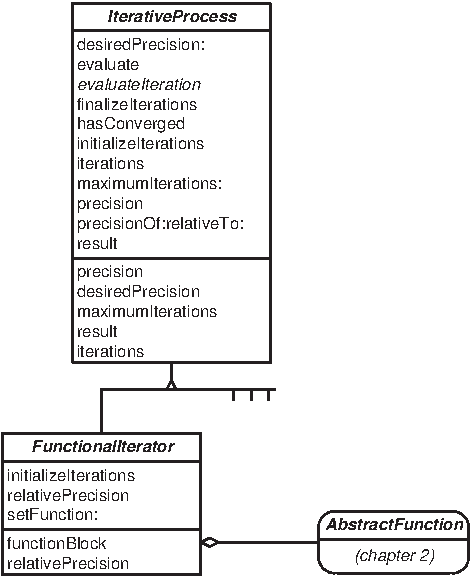
\includegraphics[width=6cm]{Figures/IterationClasses}
\caption{Class diagram for iterative process
classes}\label{cl:iteration}
\end{figure}
This chapter first discusses the implementation of a
general-purpose iterative process. Then, we describe a
generalization for the finding of a numerical result. Other
chapters discuss examples of sub-classing of these classes to
implement specific algorithms.

Iteration is used to find the solution of a wide variety of
problems other than just function evaluation. Finding the location
where a function is zero, reached a maximum or a minimum is
another example. Some data mining algorithms also use iteration to
find a solution (\cf section \ref{sec:cluster}).

\section{Successive approximations}
\label{sec:iteration} A general-purpose iterative process can be
decomposed in three main steps:
\begin{itemize}
  \item a set-up phase
  \item an iteration phase until the result is acceptable
  \item a clean-up phase
\end{itemize}
\noindent These steps are translated schematically into the flow
diagram shown in Figure \ref{fig:itercoarse}.
\begin{figure}
\centering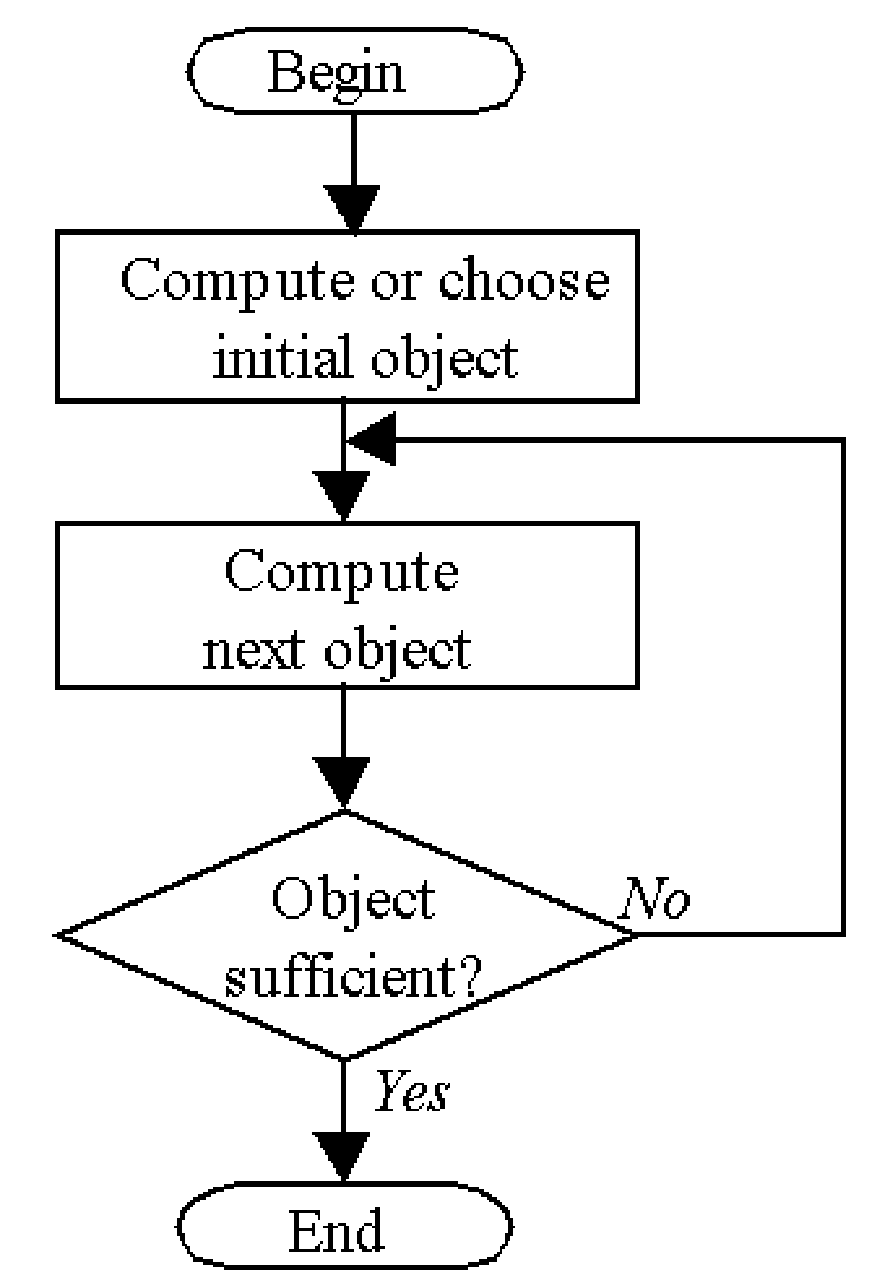
\includegraphics[width=5cm]{Figures/IterationCoarseFlow}
\caption{Successive approximation algorithm}\label{fig:itercoarse}
\end{figure}

The set-up phase allows determining constant parameters used by
the subsequent computations. Often a first estimation of the
solution is defined at this time. In any case an object
representing the approximate solution is constructed. Depending on
the complexity of the problem a class will explicitly represent
the solution object. Otherwise the solution shall be described by
a few instance variables of simple types (numbers and arrays).

After the set-up phase the iterative process proper is started. A
transformation is applied to the solution object to obtain a new
object. This process is repeated unless the solution object
resulting from the last transformation can be considered close
enough to the sought solution.

During the clean-up phase resources used by the iterative process
must be release. In some cases additional results may be derived
before leaving the algorithm.

\noindent Let us now explicit each of the three stages of the
algorithm.

The step computing or choosing an initial object is strongly
dependent on the nature of the problem to be solved. In some
methods, a good estimate of the solution can be computed from the
data. In others using randomly generated objects yields good
results. Finally, one can also ask the application's user for
directions. In many cases this step is also used to initialize
parameters needed by the algorithm.

The step computing the next object contains the essence of the
algorithm. In general a new object is generated based on the
history of the algorithm.

The step deciding whether or not an object is sufficiently close
to the sought solution is more general. If the algorithm is
capable of estimating the precision of the solution --- that is,
how close the current object is located from the exact solution
--- one can decide to stop the algorithm by comparing the
precision to a desired value. This is not always the case,
however. Some algorithms, genetic algorithms for example, do not
have a criterion for stopping.

Whether or not a well-defined stopping criterion exists, the
algorithm must be prevented from taking an arbitrary large amount
of time. Thus, the object implementing an iterative process ought
to keep track of the number of iterations and interrupt the
algorithm if the number of iterations becomes larger than a given
number.

\rubrique{Design}
%\marginpar{Figure \ref{cl:iteration} with the box {\bf IterativeProcess} grayed.}
Now we can add some details to the
algorithm. The new details are shown in figure \ref{fig:iterfine}.
\begin{figure}
\centering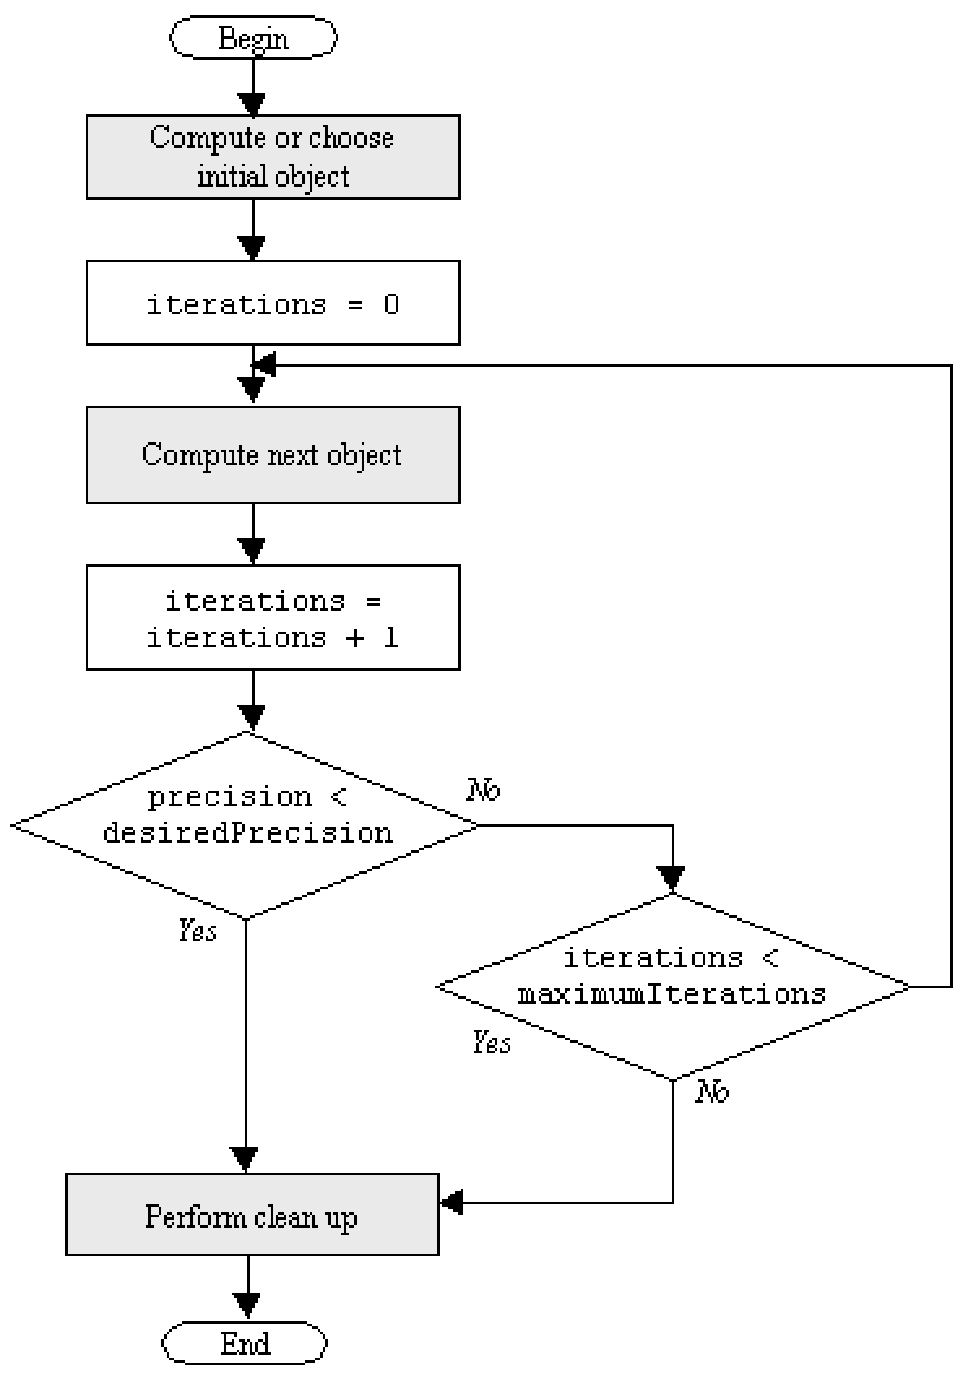
\includegraphics[width=4in]{Figures/IterationFineFlow}
\caption{Detailed algorithm for successive
approximations}\label{fig:iterfine}
\end{figure}
This schema allows us to determine the structure of a general
object implementing the iterative process. It will be implemented
as an abstract class. An abstract class is a class with does not
have object instances. A object implementing a specific algorithm
is an instance of a particular subclass of the abstract class.

The gray boxes in figure \ref{fig:iterfine} represent the methods,
which must be implemented explicitly by the subclass. The abstract
class calls them. However, the exact implementation of these
methods is not defined at this stage.
Such methods are called {\textsl hook} methods.

Using this architecture the abstract class is able to implement
the iterative process without any deep knowledge of the algorithm.
Algorithm specific methods are implemented by the subclass of the
abstract class.

Let us call \code{IterativeProcess} the class of the abstract
object. The class \code{IterativeProcess} needs the following
instance variables:
\begin{itemize}
\item \code{iterations}keeps track of the number of iterations, that is the number of successive
approximations,
\item \code{maximumIterations} maximum number of allowed iterations,
\item \code{desiredPrecision} the precision to attain, that is, how close to the solution should the solution object be when the algorithm is
terminated,
\item \code{precision} the precision achieved by the process. Its value is updated after each iteration and it is used to decide when to stop.
\end{itemize}
\begin{figure}
\centering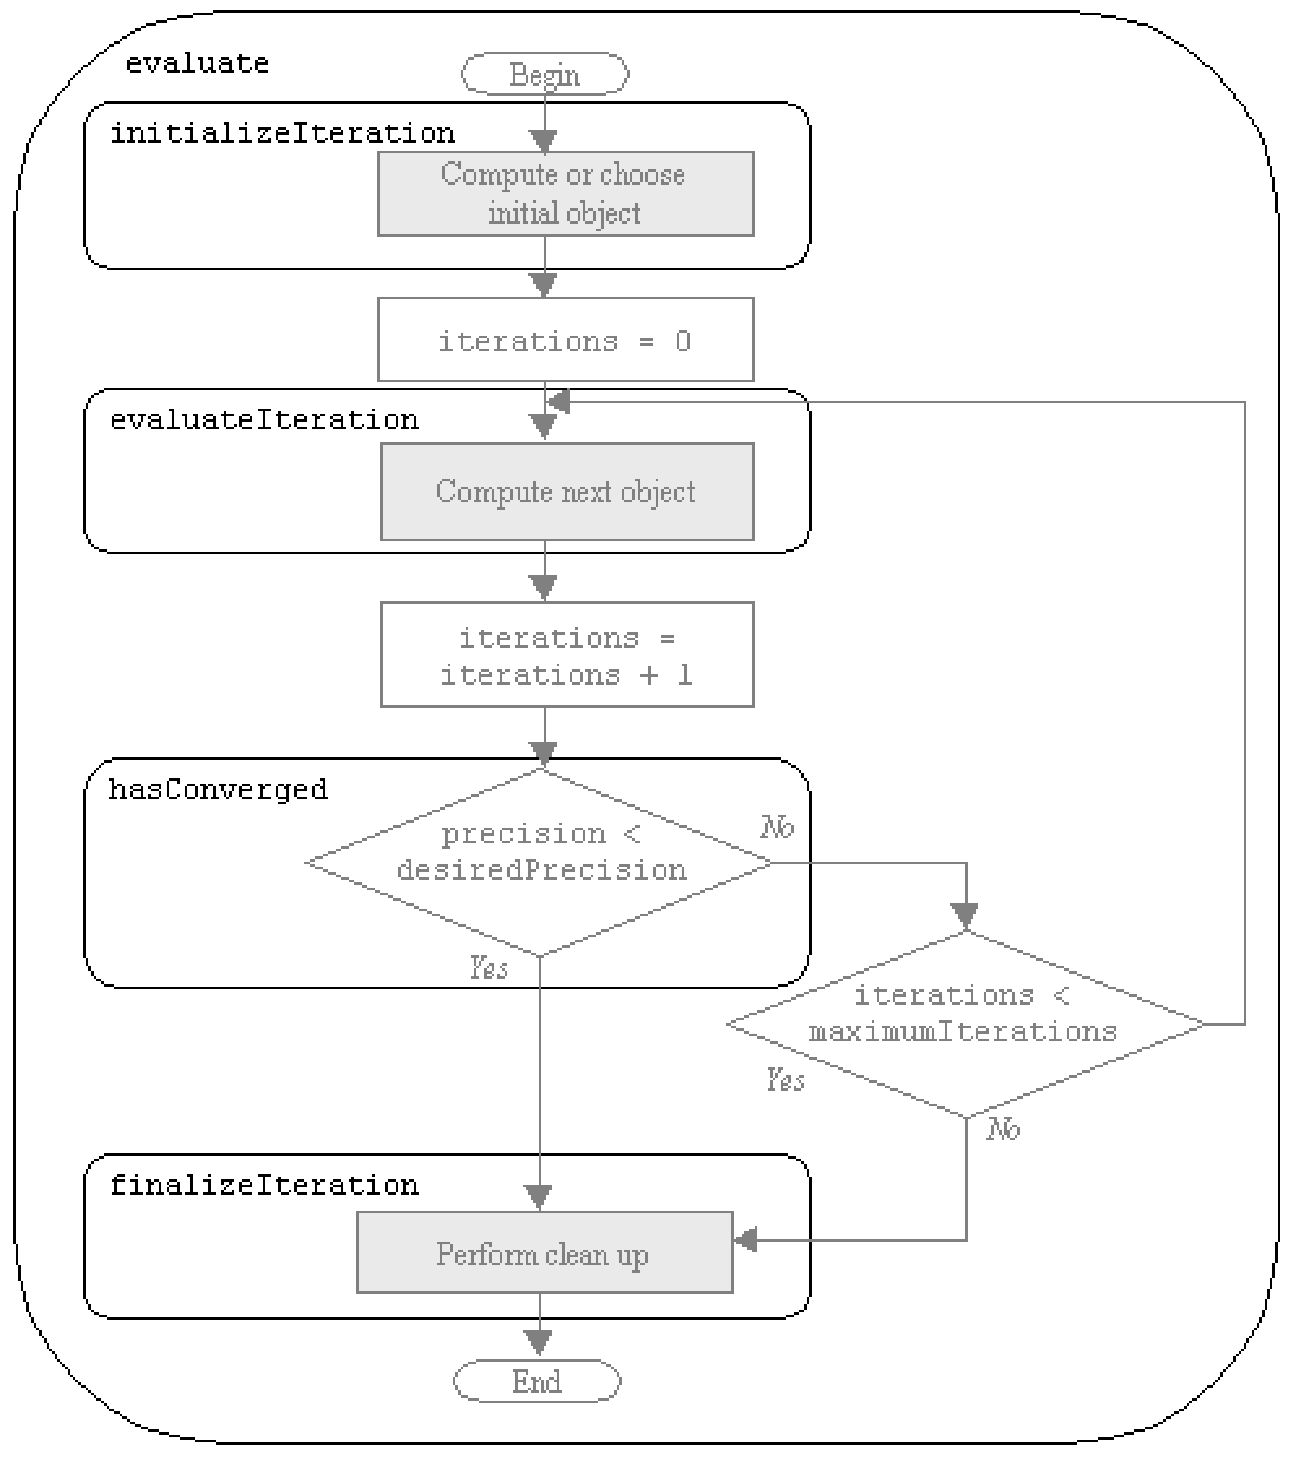
\includegraphics[width=4in]{Figures/IterationMethods}
\caption{Methods for successive
approximations}\label{fig:itermeth}
\end{figure}
The methods of the class \code{IterativeProcess} are shown in
figure \ref{fig:itermeth} in correspondence with the general
execution flow shown in figure \ref{fig:iterfine}. The two methods
\code{initializeIterations} and \code{finalizeIterations} should be
implemented by the subclass but the abstract class provides a
default behavior: doing nothing. The method \code{evaluateIteration} must be implemented by each subclass.

Since the precision of the last iteration is kept in an instance
variable, the method \code{hasConverged} can be called at any time
after evaluation, thus providing a way for client classes to check
whether the evaluation has converged or not.

\subsection{Iterative process --- Smalltalk implementation}
\label{sec:siteration}
Even though we are dealing for the moment
with an abstract class we are able to present a scenario of use
illustrating the public interface to the class. Here is how a
basic utilization of an iterative process object would look like.
\begin{displaycode}{Smalltalk}
| iterativeProcess result |
iterativeProcess := <a subclass of DhbIterativeProcess> new.
result := iterativeProcess evaluate.
iterativeProcess hasConverged
   ifFalse:[ <special case processing> ].
\end{displaycode}

The first statement creates an object to handle the iterative
process. The second one performs the process and retrieves the
result, whatever it is. The final statement checks for
convergence.

To give the user a possibility to have more control, one can
extend the public interface of the object to allow defining the
parameters of the iterative process: the desired precision and the
maximum number of iterations. In addition, the user may want to
know the precision of the attained result and the number of
iterations needed to obtain the result. The following code sample
shows an example of use for all public methods defined for an
iterative process. The precision of the attained result and the
number of iterations are printed on the transcript window.

\begin{displaycode}{Smalltalk}
| iterativeProcess result precision |
iterativeProcess := <a subclass of DhbIterativeProcess> new.
iterativeProcess desiredPrecision: 1.0e-6; maximumIterations: 25.
result := iterativeProcess evaluate.
iterativeProcess hasConverged
   ifTrue: [ Transcript nextPutAll: 'Result obtained after '.
             iterativeProcess iteration printOn: Transcript.
             Transcript nextPutAll: 'iterations. Attained precision is'.
             iterativeProcess precision printOn: Transcript.
             ]
    ifFalse:[ Transcript nextPutAll: 'Process did not converge'.].
Transcript cr.
\end{displaycode}

Listing \ref{lst:iteration} shows the Smalltalk implementation of the iterative process.

In the Smalltalk implementation, the class \code{IterativeProcess}
has one instance variable in addition to the ones described in the
preceding section. This variable, called \code{result}, is used to
keep the solution object of the process. The method \code{result}
allows direct access to it. Thus, all subclasses can use this
instance variable as a placeholder to store any type of result. As
a convenience the method \code{evaluate} also returns the instance
variable \code{result}.

Default values for the desired precision and the maximum number of
iterations are kept in class methods for easy editing. The method
initialize loads these default values for each newly created
instance. The default precision is set to the machine precision
discussed in section \ref{sec-rounding}.

The methods used to modify the desired precision (\code{desiredPrecision:}) and the maximum number of iterations (\code{maximumIterations:}) check the value to prevent illegal
definitions, which could prevent the algorithm from terminating.

Since there is no explicit declaration of abstract class and abstract methods in Smalltalk\footnote{An abstract class is a class containing at least an abstract method; an abstract method contains the single conventional statement: \code{self subclassResponsibility}} the three methods \code{initializeIterations}, \code{evaluateIteration} and \code{finalizeIterations}, are implemented with a reasonable default behavior.
The methods \code{initializeIterations} and \code{finalizeIterations} do nothing. The method \code{evaluateIteration} calls the method \code{subclassResponsibility}, which raises an
exception when called.
Using this technique is the Smalltalk way of creating an abstract method.
\begin{listing}[label=lst:iteration]{Smalltalk}
{Smalltalk implementation of an iterative process}
Object subclass: #PMIterativeProcess
   instanceVariableNames: 'precision desiredPrecision maximumIterations result iterations'
   classVariableNames: ''
   package: 'Math-Core-Process'
\end{listing}

\begin{displaycode}{Smalltalk}
PMIterativeProcess class >> defaultMaximumIterations
    ^50
\end{displaycode}

\begin{displaycode}{Smalltalk}
PMIterativeProcess class >> defaultPrecision
    ^PMFloatingPointMachine new defaultNumericalPrecision
\end{displaycode}

\begin{displaycode}{Smalltalk}
PMIterativeProcess >> desiredPrecision: aNumber
    aNumber > 0
        ifFalse: [ ^self error: 'Illegal precision: ', aNumber 
                                                         printString].
    desiredPrecision := aNumber.
\end{displaycode}

\begin{displaycode}{Smalltalk}
PMIterativeProcess >> evaluate
    iterations := 0.
    self initializeIterations.
    [iterations := iterations + 1.
    precision := self evaluateIteration.
    self hasConverged or: [iterations >= maximumIterations]] 
            whileFalse: [].
    self finalizeIterations.
    ^self result
\end{displaycode}

\begin{displaycode}{Smalltalk}
PMIterativeProcess >> evaluateIteration
    ^self subclassResponsibility
\end{displaycode}

\begin{displaycode}{Smalltalk}
PMIterativeProcess >> finalizeIterations
   "Perform cleanup operation if needed (must be implemented by subclass)."
\end{displaycode}

\begin{displaycode}{Smalltalk}
PMIterativeProcess >> hasConverged
    ^precision <= desiredPrecision
\end{displaycode}

\begin{displaycode}{Smalltalk}
PMIterativeProcess >> initialize
    desiredPrecision := self class defaultPrecision.
    maximumIterations := self class defaultMaximumIterations.
    ^self
\end{displaycode}

\begin{displaycode}{Smalltalk}
PMIterativeProcess >> initializeIterations
   "Initialize the iterations (must be implemented by subclass when needed)."
\end{displaycode}

\begin{displaycode}{Smalltalk}
PMIterativeProcess >> iterations
    ^iterations
\end{displaycode}

\begin{displaycode}{Smalltalk}
PMIterativeProcess >> maximumIterations: anInteger
    ( anInteger isInteger and: [ anInteger > 1])
        ifFalse: [ ^self error: 'Invalid maximum number of iteration: 
                                            ', anInteger printString].
    maximumIterations := anInteger
\end{displaycode}

\begin{displaycode}{Smalltalk}
PMIterativeProcess >> precision
    ^precision
\end{displaycode}

\begin{displaycode}{Smalltalk}
PMIterativeProcess >> precisionOf: aNumber1 relativeTo: aNumber2
    ^aNumber2 > PMFloatingPointMachine new defaultNumericalPrecision
        ifTrue: [ aNumber1 / aNumber2]
        ifFalse:[ aNumber1]
\end{displaycode}

\begin{displaycode}{Smalltalk}
PMIterativeProcess >> result
   ^result
\end{displaycode}

\begin{quote}
{\textbf Note:} The method \code{precisionOf:relativeTo:} implements
the computation of the relative precision. This is discussed in
section \ref{sec:siterrel}.
\end{quote}


\section{Evaluation with relative precision}
\label{sec:iterrel}
%\marginpar{Figure \ref{cl:iteration} with the box {\bf FunctionalIterator} grayed.}
So far we have made no
assumption about the nature of the solution searched by an
iterative process. In this section we want to discuss the case
when the solution is a numerical value.

As discussed in section \ref{sec-rounding} a floating-point number
is a representation with constant relative precision. It is thus
meaningless to use absolute precision to determine the convergence
of an algorithm. The precision of an algorithm resulting in a
numerical value ought to be determined relatively.

One way to do it is to have the method \code{evaluateIteration}
returning a relative precision instead of an absolute number.
Relative precision, however, can only be evaluated if the final
result is different from zero. If the result is zero, the only
possibility is to check for absolute precision. Of course, in
practice one does not check for equality with zero. The
computation of a relative precision is carried only if the
absolute value of the result is larger than the desired precision.

The reasoning behind the computation of the relative error is
quite general. Thus, a general-purpose class \code{FunctionalIterator} has been created to implement a method
computing the relative precision from an absolute precision and a
numerical result. In addition, since all subclasses of \code{FunctionalIterator} use a function a general method to handle the
definition of that function is also supplied.

\subsection{Relative precision --- Smalltalk  implementation}
\label{sec:siterrel} In this case the public interface is extended
with a creation method taking as argument the function on which
the process operates.
The code example of section \ref{sec:siteration} then becomes:
\begin{displaycode}{Smalltalk}
| iterativeProcess result |
iterativeProcess := <a subclass of PMFunctionalIterator>
                  function: ( PMPolynomial coefficients: #(1 2 3)).
result := iterativeProcess evaluate.
iterativeProcess hasConverged ifFalse:[ <special case processing>].
\end{displaycode}
In this example the function on which the process will operate is
the polynomial $3x^2+2x+1$ (\cf section \ref{sec:polynomial}).

Listing \ref{ls:iterrel} shows the implementation of the abstract
class \code{PMFunctionalIterator} in Smalltalk.

This class has one instance variable \code{functionBlock} to store
the function. A single class method allows creating a new instance
while defining the function.

As we have seen in section \ref{sec:stFunction}, a function can be
any object responding to the message value:. This allows supplying
any block of Smalltalk code as argument to the constructor method.
However, the user can also supply a class implementing the
computation of the function with a method with selector \code{value:}. For example, an instance of the class \code{PMPolynomial}
discussed in section \ref{sec:stPolynomial} can be used.

The instance method \code{setFunction:} is used to set the instance
variable \code{functionBlock}. In order to prevent a client class
from sending the wrong object, the method first checks whether the
supplied object responds to the message \code{value:}. This is one
way of ensuring that the arguments passed to a method conform to
the expected protocol. This way of doing is only shown as an
example, however. It is not recommend in practice. The
responsibility of supplying the correct arguments to a Smalltalk
method is usually the responsibility of the client class.

The method \code{initializeIterations} first checks whether a
function block has been defined. Then it calls the method \code{computeInitialValues}. This method is a hook method, which a
subclass must implement to compute the value of the result at the
beginning of the iterative process.

The computation of relative precision is implemented at two
levels. One general method, \code{precisionOf:relativeTo:},
implemented by the superclass allows the computation of the
relative precision relative to any value. Any iterative process
can use this method. The method \code{relativePrecision} implements
the computation of the precision relative to the current result.

\begin{listing}[label=lst:iterrel]{Smalltalk}
{Smalltalk implementation of the class PMFunctionalIterator}
PMIterativeProcess subclass: #PMFunctionalIterator
   instanceVariableNames: 'functionBlock'
   classVariableNames: ''
   package: 'Math-DHB-Numerical-Math-FunctionIterator'
\end{listing}

\begin{displaycode}{Smalltalk}
PMFunctionalIterator class >> function: aBlock
    ^self new setFunction: aBlock; yourself
\end{displaycode}

\begin{displaycode}{Smalltalk}
PMFunctionalIterator >> initializeIterations
    functionBlock isNil ifTrue: [self error: 'No function supplied'].
    self computeInitialValues
\end{displaycode}

\begin{displaycode}{Smalltalk}
PMFunctionalIterator >> relativePrecision: aNumber
    ^self precisionOf: aNumber relativeTo: result abs
\end{displaycode}

\begin{displaycode}{Smalltalk}
PMFunctionalIterator >> setFunction: aBlock
    ( aBlock respondsTo: #value:)
        ifFalse:[ self error: 'Function block must implement the 
                                                      method value:'].
    functionBlock := aBlock
\end{displaycode}

\section{Examples}
As we have dealt with abstract classes, this chapter did not give
concrete examples of use. By consulting the rest of this book the
reader will find numerous examples of subclasses of the two
classes described in this chapter. Table \ref{tb:iteration} lists
the sections where each algorithm using the iterative process
framework is discussed.
\begin{table}[h]
  \centering
  \caption{Algorithms using iterative processes}\label{tb:iteration}
\vspace{1 ex}
\begin{tabular}{|l|l|c|} \hline
\textbf{Algorithm or class of algorithm}&\textbf{Superclass}&\textbf{
Chapter or section}
\\ \hline Zero finding&Function iterator&Chapter \ref{ch:zeroes}
\\ \hline Integration&Function iterator&Chapter
\ref{ch:integration}
\\ \hline Infinite series and continued fractions&Function
iterator&Chapter \ref{ch:series}  \\ \hline Matrix
eigenvalues&Iterative process&Section \ref{sec:eigen}
\\ \hline Non-linear least square fit&Iterative process&Section
\ref{sec:lsfnonlin}
\\ \hline Maximum likelihood fit&Iterative process&Section \ref{sec:mlfhist} \\
\hline Function minimization&Function iterator&Chapter
\ref{ch:minimization}  \\ \hline Cluster analysis&Iterative
process&Section \ref{sec:cluster} \\ \hline
\end{tabular}

\end{table}

%\ifx\wholebook\relax\else\end{document}\fi

%\ifx\wholebook\relax\else
%\documentclass[twoside]{book}
%\usepackage[active]{srcltx}
%\usepackage[LY1]{fontenc}
%\usepackage{url}
\makeatletter
\def\url@leostyle{%
  \@ifundefined{selectfont}{\def\UrlFont{\sf}}{\def\UrlFont{\sffamily}}}
\makeatother
% Now actually use the newly defined style.
\urlstyle{leo}

\usepackage{graphicx}
\def\etc{{\textit{etc}}}
\def\eg{{\textit{e.g.}}}
\def\ie{{\textit{i.e.}}}
\def\cf{{\textit{c.f.}}\ }
\def\erf{\mathop{\textrm{erf}}}
\def\sign{\mathop{\textrm{sign}}}
\def\prob{\mathop{\textrm{Prob}}}
\def\var{\mathop{\textrm{var}}}
\def\mod{\mathop{\textrm{mod}}}
\def\cor{\mathop{\textrm{cor}}}
\def\cov{\mathop{\textrm{cov}}}
\def\cl{\mathop{\textrm{CL}}}
\def\kg{\mathop{\textrm{Kg}}}
\def\patstyle#1{{\textsc #1}}
\def\th{^{\mathop{\textrm{th}}}}
%\def\st#1{^{\mathop{\rm #1}}}
\def\note#1{\begin{quote}{\textbf{Note:}} #1\end{quote}}
\def\braket#1{\left\langle #1\right\rangle}
\def\order#1{\let\o=#1$\mathcal{O}$\ifx\o 1$\left(n\right)$\else$\left(n^{#1}\right)$\fi}
%\newtheorem{privListing}{Listing}[chapter]
%\newenvironment{listing}{\vskip 3ex\hrule\vskip 1ex\begin{privListing}}{\end{privListing}\hrule\vskip 1ex}
\newtheorem{privExample}{Code example}[chapter]
\newenvironment{codeExample}{\begin{privExample}\begin{quote}\tt}{\end{quote}\end{privExample}}
\def\relboxl#1#2{\hbox to #1\hsize{#2\hfil}}
\def\relboxc#1#2{\hbox to #1\hsize{\hfil #2\hfil}}
\def\relboxr#1#2{\hbox to #1\hsize{\hfil #2}}
\def\transpose#1{\textbf{#1}^{\mathop\textrm{T}}}
\def\inverse#1{\textbf{#1}^{-1}}
%\def\tm{$^{\mathop{\rm TM}}$}
\def\tm{ }
\newenvironment{mainEquation}{\marginpar[\vspace{3 ex} Main
equation$\Rightarrow$]{\vspace{3 ex}$\Leftarrow$Main
equation}\begin{equation}}{\end{equation}}
\def\rubrique#1{\paragraph{#1}\hfil\par\noindent}

%\begin{document}
%\fi

\chapter{Finding the zero of a function}
\label{ch:zeroes} \vspace{1 ex}
\begin{flushright} {\textsl Le z\'ero, collier du n\'eant.}\footnote{The zero, a necklace for emptiness.}\\ Jean Cocteau
\end{flushright}
\vspace{1 ex}
The zeroes of a function are the values of the
function's variable for which the value of the function is zero.
Mathematically, given the function $f\left(x\right)$, $z$ is a
zero of when $f\left(z\right)=0$. This kind of problem is can be
extended to the general problem of computing the value of the
inverse function, that is finding a value $x$ such that
$f\left(x\right)=c$ where $c$ is a given number. The inverse
function is noted as $f^{-1}\left(x\right)$. Thus, one wants to
find the value of $f^{-1}\left(c\right)$ for any $c$. The problem
can be transformed into the problem of finding the zero of the
function $\tilde{f}\left(x\right)=f\left(x\right)-c$.

The problem of finding the values at which a function takes a
maximum or minimum value is called searching for the extremes of a
function. This problem can be transformed into a zero-finding
problem if the derivative of the function can be easily computed.
The extremes are the zeroes of the function's derivative.

\noindent Figure \ref{cl:zeroFinding} shows the class diagram of
the classes discussed in this chapter.
\begin{figure}
\centering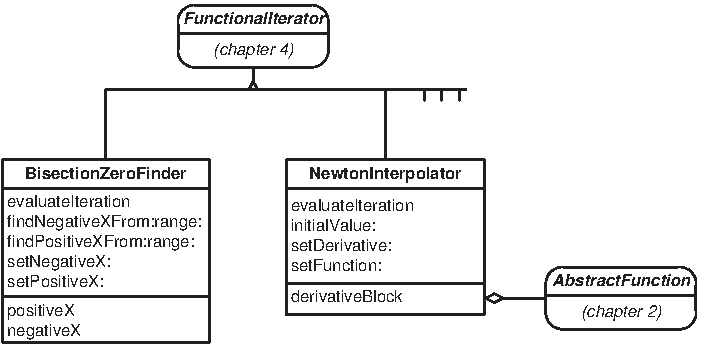
\includegraphics[width=10cm]{Figures/ZeroClassDiagram}
\caption{Class diagram for zero finding
classes}\label{cl:zeroFinding}
\end{figure}


\section{Introduction}
Let us begin with a concrete example.

Often an experimental result is obtained by measuring the same
quantity several times. In scientific publications, such a result
is published with two numbers: the average and the standard
deviation of the measurements. This is true for medical
publication as well. As we have already discussed in section
\ref{sec:errorFunctionDef}, obstetricians prefer to think in terms
of risk and prefer to use centiles instead of average and standard
deviation. Assuming that the measurements were distributed
according to a normal distribution (\cf section
\ref{sec:normdist}), the 90th centile is the solution to the
following equation:
\begin{equation}
\label{eq:centile90}
  \erf\left(x\right)=0.9
\end{equation}
That is, we need to find the zero of the function
$f\left(x\right)=\erf\left(x\right)-0.9$. The answer is $x=1.28$
with a precision of two decimals. Thus, if $\mu$ and $\sigma$ are
respectively the average and standard deviation of a published
measurement, the 90th centile is given by $\mu+1.28\cdot\sigma$.
Using equation \ref{eq:erfneg} the 10th centile is given by
$\mu-1.28\cdot\sigma$.

\section{Finding the zeroes of a function --- Bisection method}
\label{sec:bisection}
%\marginpar{Figure \ref{cl:zeroFinding} with the box {\textbf BisectionZeroFinder} grayed.}
Let assume that one knows two values of $x$ for which the function takes values of
opposite sign. Let us call $x_{pos}$ the value such
that $f\left(x_{pos}\right)>0$ and $x_{neg}$ the value such that $f\left(x_{neg}\right)<0$.
If the function is continuous between $x_{pos}$ and
$x_{neg}$, there exists at least one zero of the
function in the interval $\left[ x_{pos},x_{neg}\right]$. This is illustrated in figure
\ref{fig:bisection}. If the function $f$ is not continuous over
the interval where the sign of the function changes, then the
presence of a zero cannot be guaranteed\footnote{The inverse
function is such an example. It changes sign over 0 but has no
zeroes for any finite $x$}. The continuity requirement is
essential for the application of the bisection algorithm.

The values $x_{pos}$ and $x_{neg}$ are
the initial values of the bisection algorithm. The algorithm goes
as follows:
\begin{enumerate}
  \item Compute $x={x_{pos}-x_{neg}\over2}$.
  \item If $f\left(x\right)>0$, set $x_{pos}=x$ and
  goto step 4.
  \item Otherwise set $x_{neg}=x$.
  \item If $\left|x_{pos},x_{neg}\right|>\epsilon$ go back
to step 1. $\epsilon$ is the desired precision of the solution.
\end{enumerate}
The first couple of steps of the bisection algorithm are
represented geometrically on figure \ref{fig:bisection}. Given the
two initial values, $x_{pos}$ and $x_{neg}$, the first iteration of the algorithm replaces $x_{pos}$ with $x_1$. The next step replaces $x_{neg}$ with $x_2$.
\begin{figure}
\centering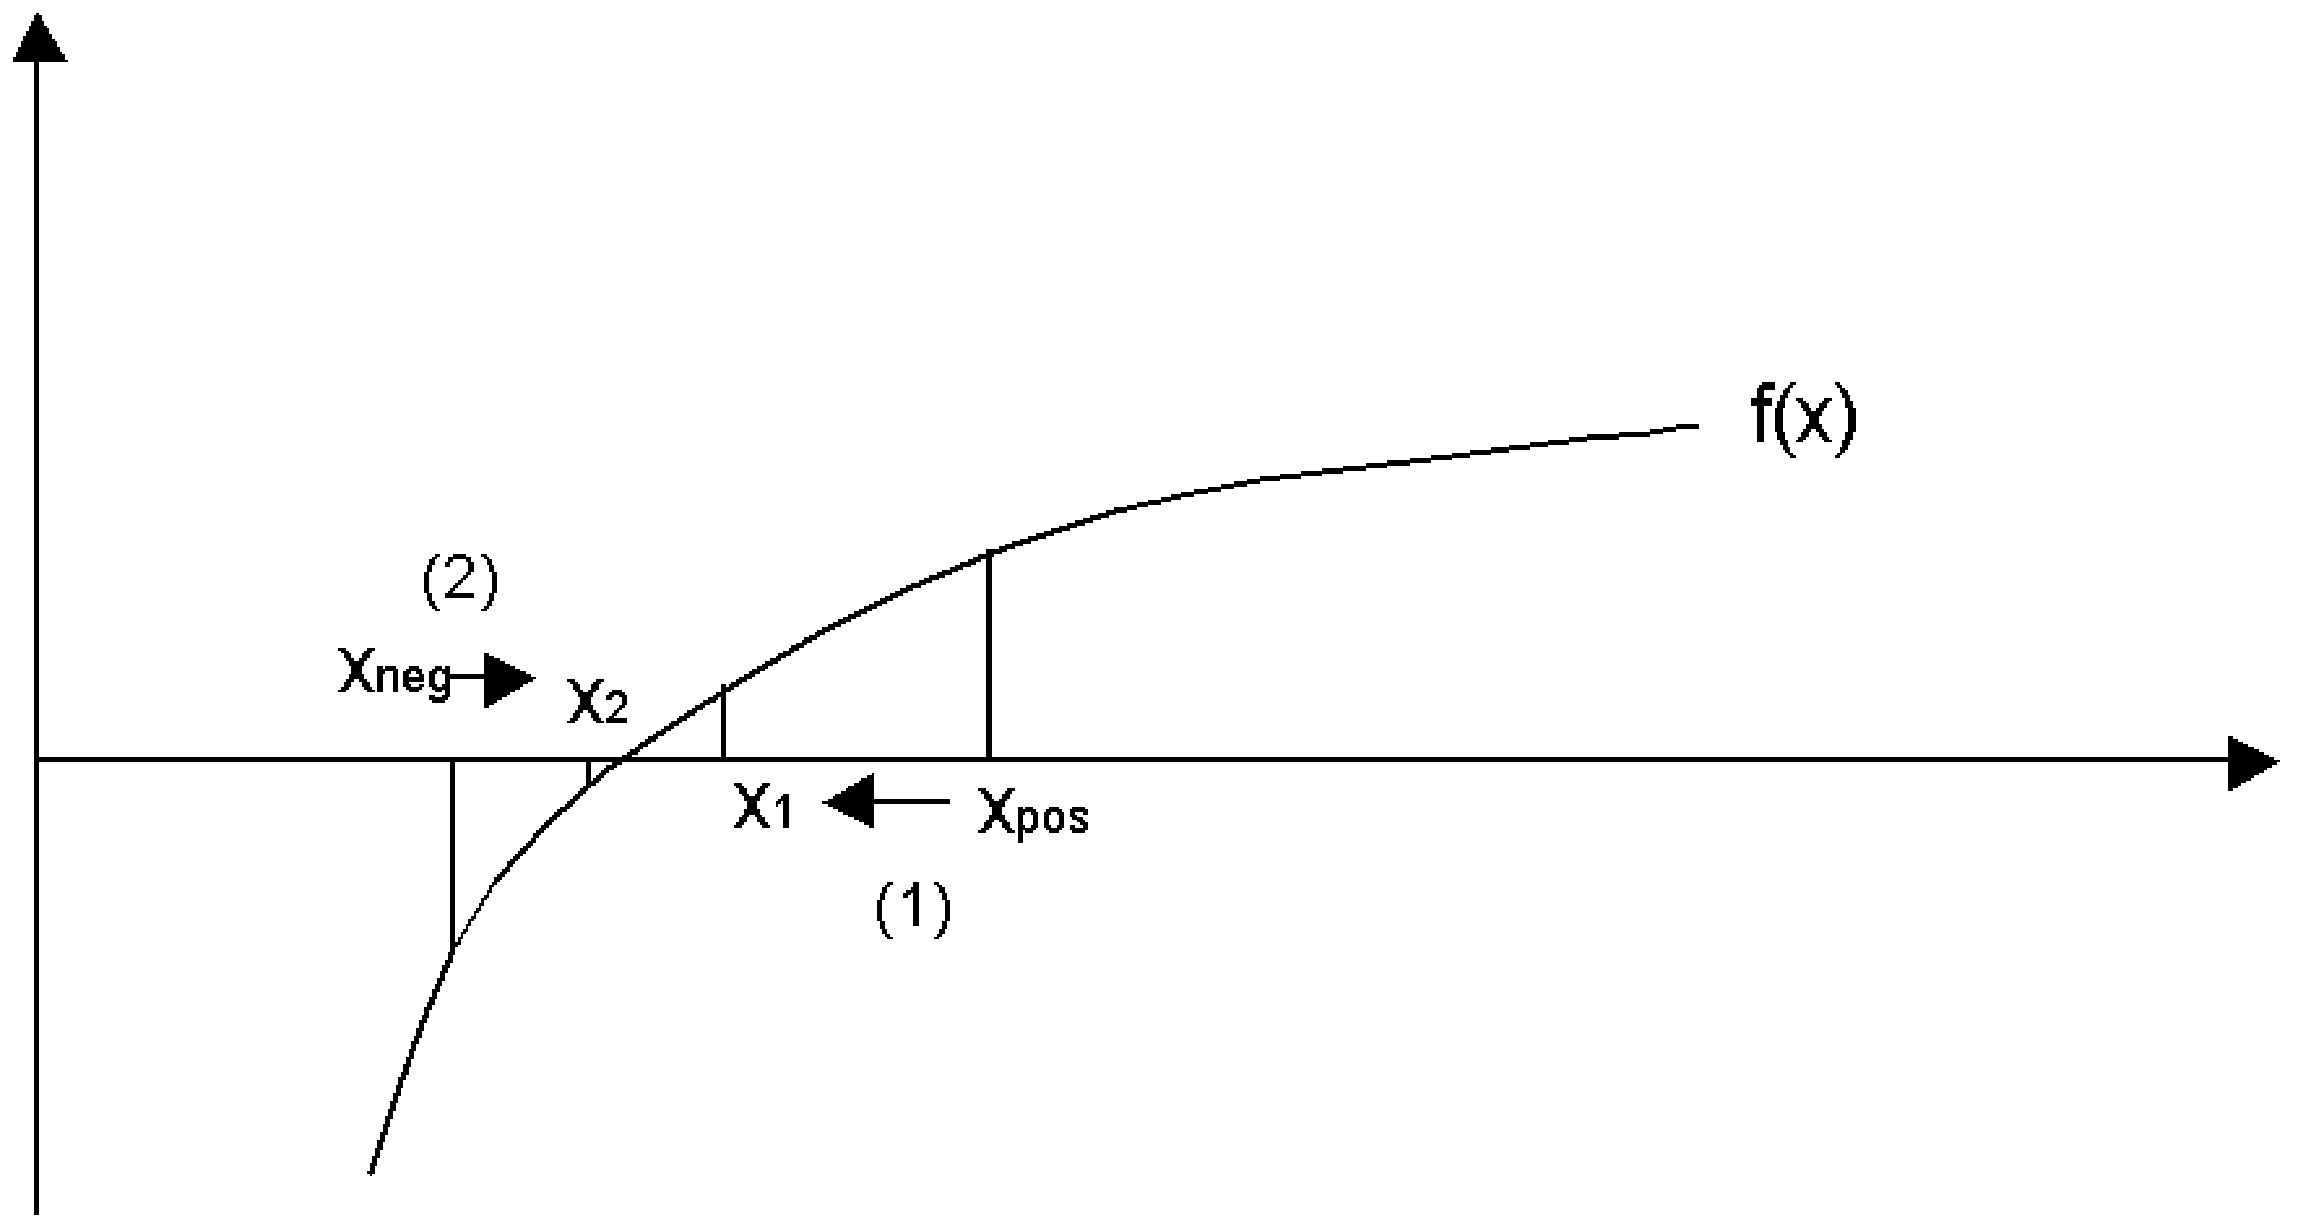
\includegraphics[width=12cm]{Figures/BissectionGraph}
\caption{The bisection algorithm}\label{fig:bisection}
\end{figure}

For a given pair of initial values, $x_{pos}$ and $x_{neg}$, the number of iterations required to attain a precision $\epsilon$ is given by:
\begin{equation}
\label{eq:bissectime}
  n=\left\lceil\log_2{\displaystyle\left| x_{pos},x_{neg}\right| \over
\displaystyle\epsilon}\right\rceil.
\end{equation}
For example if the distance between the two initial values is 1
the number of iterations required to attain a precision of
$10^{-8}$ is 30. It shows that the bisection algorithm is rather
slow.

Knowledge of the initial values, $x_{pos}$ and $x_{neg}$, is essential for starting the algorithm.
Methods to define them must be supplied. Two convenience methods
are supplied to sample the function randomly over a given range to
find each initial value. The random number generator is discussed
in section \ref{sec:random}.

The bisection algorithm is a concrete implementation of an
iterative process. In this case, the method \code{evaluateIteration} of figure \ref{fig:itermeth} implements steps
2, 3 and 4. The precision at each iteration is $\left|
x_{pos}-x_{neg}\right|$ since the zero
of the function is always inside the interval defined by
$x_{pos}$ and $x_{neg}$.

\subsection{Bisection algorithm --- General  implementation}

The class of the object implementing the bisection algorithm is a
subclass of the abstract class \code{FunctionalIterator}.
The class \code{BisectionZeroFinder} needs the following additional instance variables.
\begin{description}
  \item[\texttt positiveX]$x_{pos}$ and
  \item [\texttt negativeX]$x_{neg}$
\end{description}
The bisection algorithm proper is implemented only within the
method \code{evaluateIteration}.
Other necessary methods have already been implemented in the iterative process class.

\subsection{Bisection algorithm --- Smalltalk  implementation}
Finding the zero of a function is performed by creating an
instance of the class \code{PMBisectionZeroFinder} and giving the
function as the argument of the creation method as explained in
section \ref{sec:siterrel}. For example the following code finds
the solution of equation \ref{eq:centile90}.
\begin{displaycode}{Smalltalk}
| zeroFinder result |
zeroFinder:= PMBisectionZeroFinder function: [ :x | x errorFunction - 0.9].
zeroFinder setPositiveX: 10; setNegativeX: 0.
result := zeroFinder evaluate. zeroFinder
hasConverged
   ifFalse:[ <special case processing>].
\end{displaycode}
The second line creates the object responsible to find the zero.
The third line defines the initial values, $x_{pos}$ and $x_{neg}$.
The fourth line performs the algorithm and stores the result if the algorithm has converged.
The last two lines check for convergence and take corrective action if the algorithm did not converge.

Listing \ref{ls:bisection} shows the implementation of the bisection zero finding algorithm in Smalltalk.

The class \code{PMBisectionZeroFinder} is a subclass of the class \code{PMFunctionalIterator}. As one can see only a few methods need to be implemented.
Most of them pertain to the definition of the initial interval.
In particular, convenience methods are supplied to find a positive and negative function value over a given interval.

The methods defining the initial values, $x_{pos}$ and $x_{neg}$, are \code{setPositiveX:} and \code{setNegativeX:} respectively.
An error is generated in each method if the function's value does not have the proper sign.
The convenience methods to find random starting values are respectively \code{findPositiveXFrom:range:} and \code{findNegativeXFrom:range:}.
The method \code{computeInitialValues} does not compute the initial values. Instead it makes sure that $x_{pos}$ and $x_{neg}$ have been properly defined.

\begin{listing} Smalltalk implementation of the bisection algorithm \label{ls:bisection}
$$\halign{ #\hfil&\quad#\hfil\cr {\sl Class}& {\Large\bf DhbBisectionZeroFinder}\cr
{\sl Subclass of }&{\tt DhbFunctionalIterator}\cr\noalign{\vskip 1ex}

{\sl Instance variable names:}&\parbox[t]{4 in}{\tt  positiveX negativeX }\cr\noalign{\vskip 1ex}}$$


Instance methods
{\parskip 1ex\par\noindent}
{\bf computeInitialValues}
\begin{verbatim}
    positiveX isNil
        ifTrue: [ self error: 'No positive value supplied'].
    negativeX isNil
        ifTrue: [ self error: 'No negative value supplied'].

\end{verbatim}
{\bf evaluateIteration}
\begin{verbatim}
    result := ( positiveX + negativeX) * 0.5.
    ( functionBlock value: result) > 0
        ifTrue: [ positiveX := result]
        ifFalse:[ negativeX := result].
    ^self relativePrecision: ( positiveX - negativeX) abs

\end{verbatim}
{\bf findNegativeXFrom:} {\tt aNumber1} {\bf range:} {\tt aNumber2}
\begin{verbatim}
    | n |
    n := 0.
    [ negativeX := Number random * aNumber2 + aNumber1.
      ( functionBlock value: negativeX) < 0
        ] whileFalse: [ n := n + 0.1.
                        n > maximumIterations
                            ifTrue: [ self error: 'Unable to find a 
                                            negative function value'].
                      ].

\end{verbatim}
{\bf findPositiveXFrom:} {\tt aNumber1} {\bf range:} {\tt aNumber2}
\begin{verbatim}
    | n |
    n := 0.
    [ positiveX := Number random * aNumber2 + aNumber1.
      ( functionBlock value: positiveX) > 0
        ] whileFalse: [ n := n + 1.
                        n > maximumIterations
                            ifTrue: [ self error: 'Unable to find a 
                                            positive function value'].
                      ].

\end{verbatim}
{\bf setNegativeX:} {\tt aNumber}
\begin{verbatim}
    ( functionBlock value: aNumber) < 0
        ifFalse:[ self error: 'Function is not negative at x = ', 
                                                 aNumber printString].
    negativeX := aNumber.

\end{verbatim}
{\bf setPositiveX:} {\tt aNumber}
\begin{verbatim}
    ( functionBlock value: aNumber) > 0
        ifFalse:[ self error: 'Function is not positive at x = ', 
                                                 aNumber printString].
    positiveX := aNumber.

\end{verbatim}


\end{listing}

\section{Finding the zero of a function --- Newton's method}
\label{sec:newton}
%\marginpar{Figure \ref{cl:zeroFinding} with the box {\bf NewtonZeroFinder} grayed.}
Isaac Newton has designed an algorithm working by successive approximations\cite{Bass}.
Given a value $x_0$ chosen in the vicinity of the desired zero, the following series:
\begin{mainEquation}
\label{eq:newtonZero}
  x_{n+1}=x_n-{f\left(x_n\right)\over f^{\prime}\left(x_n\right)},
\end{mainEquation}
where $f^{\prime}\left(x\right)$ is the first derivative of $f\left(x\right)$, converges toward a zero of the function.
This algorithm is sometimes called Newton-Ralphson\cite{Press}.

Figure \ref{fig:newtonZero} shows the geometrical interpretation
of the series. $f^{\prime}\left(x\right)$ is the slope of the
tangent to the curve of the function $f\left(x\right)$ at the
point $x_n$. The equation of this tangent is thus given by:
\begin{figure}
\centering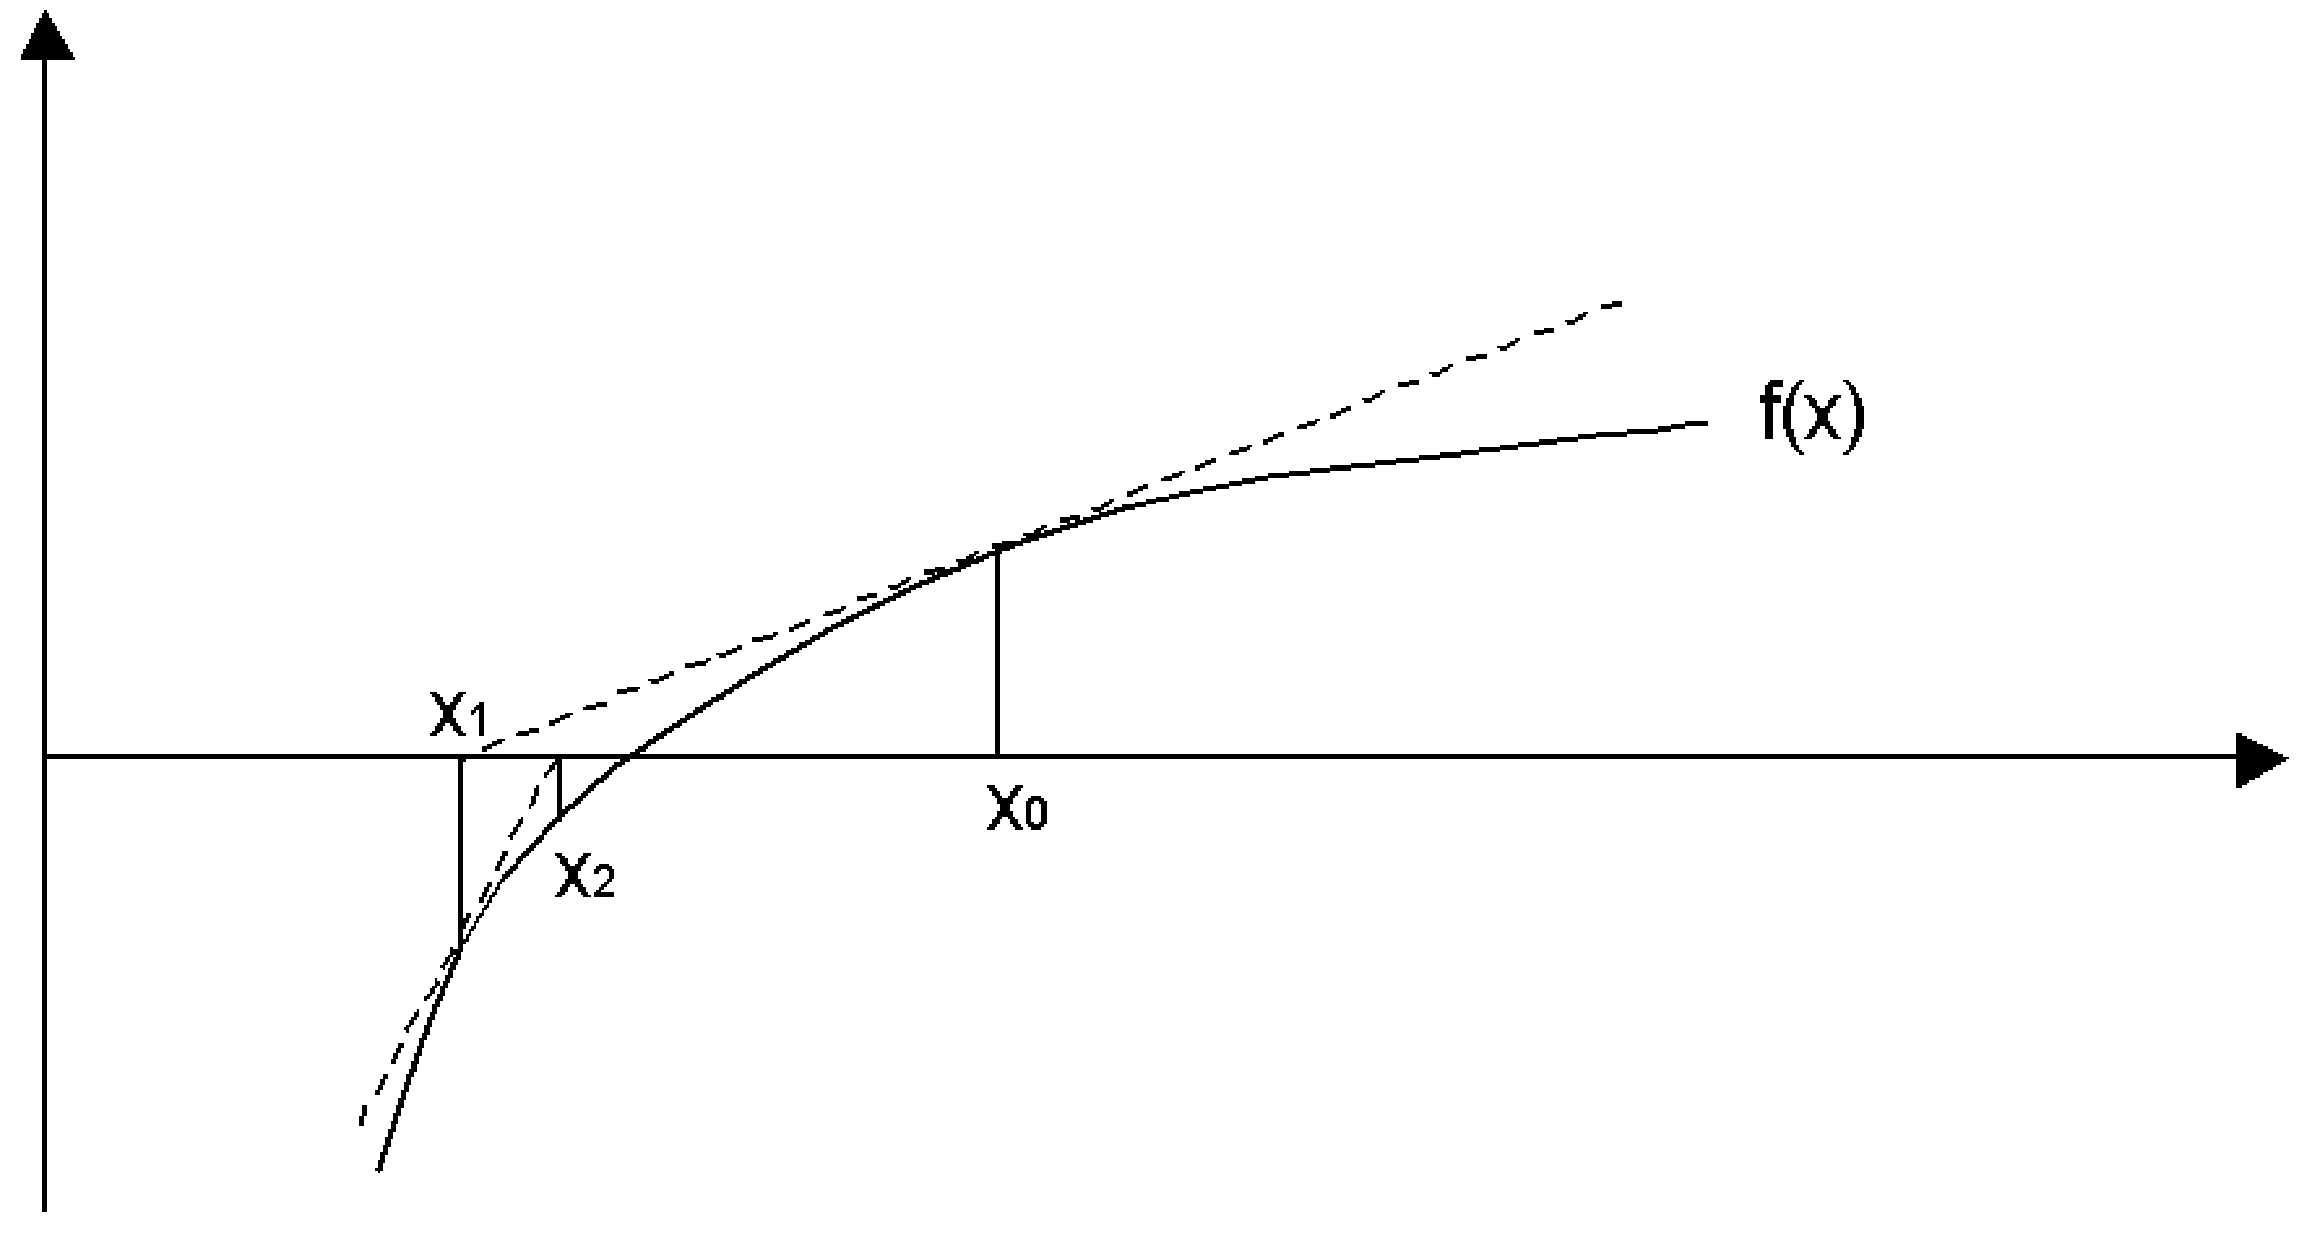
\includegraphics[width=12cm]{Figures/NewtonGraph}
\caption{Geometrical representation of Newton's zero finding
algorithm}\label{fig:newtonZero}
\end{figure}
\begin{equation}
  y=\left(x-x_n\right)\cdot f^{\prime}\left(x_n\right)+f\left(x_n\right)
\end{equation}
One can then see that $x_{n+1}$ is the point where the tangent to
the curve at the point $x_n$ crosses the $x$-axis. The algorithm
can be started at any point where the function's derivative is
non- zero.

The technique used in Newton's algorithm is a general technique
often used in approximations. The function is replaced by a linear
approximation\footnote{Mathematically, this corresponds to
estimate the function using the first two terms of its Taylor
series.}, that is a straight line going through the point defined
by the preceding value and its function's value. The slope of the
straight line is given by the first derivative of the function.
The procedure is repeated until the variation between the new
value and the preceding one is sufficiently small.
We shall see other examples of this technique in the remainder of this book
(\cf sections \ref{sec:lsfnonlin}, \ref{sec:mlfhist} and
\ref{sec:optimum}).

From equation \ref{eq:newtonZero}, one can see that the series may
not converge if $f^{\prime}\left(x\right)$ becomes zero. If the
derivative of the function is zero in the vicinity of the zero,
the bisection algorithm gives better results. Otherwise Newton's
algorithm is highly efficient. It usually requires 5-10 times less
iteration than the bisection algorithm. This largely compensates
for the additional time spent in computing the derivative.

The class implementing Newton's algorithm belongs to a subclass of
the functional iterator described in section \ref{sec:iterrel}. An
additional instance variable is needed to store the function's
derivative.

\subsection{Newton's method --- Smalltalk implementation}
\label{sec:snewton} Listing \ref{ls:newtonZero} shows the complete
implementation in Smalltalk. The class \code{PMNewtonZeroFinder}
is a subclass of the class \code{PMFunctionalIterator} described
in section \ref{sec:siterrel}. For example the following code
finds the solution of equation \ref{eq:centile90}.

\begin{displaycode}{Smalltalk}
| zeroFinder result |
zeroFinder:= DhbNewtonZeroFinder
            function: [ :x | x errorFunction - 0.9]
            derivative: [ :x | DhbErfApproximation new normal: x].
zeroFinder initialValue: 1.
result := zeroFinder evaluate.
zeroFinder hasConverged
   ifFalse:[ <special case processing>].
\end{displaycode}
The second line creates the object responsible to find the zero
supplying the function and the derivative\footnote{As we have seen
in section \ref{sec:errorFunction}, the normal distribution is the
derivative of the error function.}. The third line defines the
starting value. The fourth line performs the algorithm and stores
the result if the algorithm has converged. The last two lines
check for convergence and take corrective action if the algorithm
did not converge.

The method \code{computeInitialValues} is somewhat complex. First,
it checks whether the user supplied an initial value. If not, it
is assigned to 0. Then the method checks whether the user supplied
a derivative. If not a default derivative function is supplied as
a block closure by the method \code{defaultDerivativeBlock}. The
supplied block closure implements the formula of equation
\ref{eq:derivative}.

\begin{mainEquation}
\label{eq:derivative} {df\left(x\right)\over dx}=\lim_{\epsilon\to
0}{f\left(x+\epsilon\right)-f\left(x-\epsilon\right)\over
2\epsilon}.
\end{mainEquation}

If a derivative is supplied, it is compared to the result of the
derivative supplied by default. This may save a lot of trouble if
the user made an error in coding the derivative. Not supplying a
derivative has some negative effect on the speed and limits the
precision of the final result. The method \code{initializeIterations} also checks whether the derivative is nearly
zero for the initial value. If that is the case, the initial value
is changed with a random walk algorithm. If no value can be found
such that the derivative is non-zero an error is generated.

If the function is changed, the supplied derivative must be
suppressed. Thus, the method \code{setFunction:} must also force a
redefinition of the derivative. A method allows defining the
initial value. A creation method defining the function and
derivative is also supplied for convenience.

Like for the bisection, the algorithm itself is coded within the
method \code{evaluateIteration}. Other methods needed by the
algorithm have been already implemented in the superclasses.
\begin{listing} Smalltalk implementation of Newton's zero-finding method \label{ls:newtonZero}
$$\halign{ #\hfil&\quad#\hfil\cr {\sl Class}& {\Large\bf DhbNewtonZeroFinder}\cr
{\sl Subclass of }&{\tt DhbFunctionalIterator}\cr\noalign{\vskip 1ex}

{\sl Instance variable names:}&\parbox[t]{4 in}{\tt  derivativeBlock }\cr\noalign{\vskip 1ex}}$$


Class methods
{\parskip 1ex\par\noindent}
{\bf function:} {\tt aBlock1} {\bf derivative:} {\tt aBlock2}
\begin{verbatim}
    ^(self new) setFunction: aBlock1; setDerivative: aBlock2; 
                                                              yourself

\end{verbatim}



Instance methods
{\parskip 1ex\par\noindent}
{\bf computeInitialValues}
\begin{verbatim}
    | n |
    result isNil
        ifTrue: [ result := 0].
    derivativeBlock isNil
        ifTrue: [ derivativeBlock := self defaultDerivativeBlock].
    n := 0.
    [ (derivativeBlock value: result) equalsTo: 0]
        whileTrue: [ n := n + 1.
                     n > maximumIterations
                        ifTrue: [ self error: 'Function''s derivative 
                                        seems to be zero everywhere'].
                     result := Number random + result].

\end{verbatim}
{\bf defaultDerivativeBlock}
\begin{verbatim}
    ^[ :x | 5000 * ( ( functionBlock value: (x + 0.0001)) - ( 
                                  functionBlock value: (x - 0.0001)))]

\end{verbatim}
{\bf evaluateIteration}
\begin{verbatim}
    | delta |
    delta := ( functionBlock value: result) / ( derivativeBlock 
                                                       value: result).
    result := result - delta.
    ^self relativePrecision: delta abs

\end{verbatim}
{\bf initialValue:} {\tt aNumber}
\begin{verbatim}
    result := aNumber.

\end{verbatim}
{\bf setDerivative:} {\tt aBlock}
\begin{verbatim}
    | x |
    ( aBlock respondsTo: #value:)
        ifFalse:[ self error: 'Derivative block must implement the 
                                                      method value:'].
    x := result ifNil: [ Number random] ifNot: [ :base | base + 
                                                       Number random].
    ( ( aBlock value: x) relativelyEqualsTo: (self 
                        defaultDerivativeBlock value: x) upTo: 0.0001)
        ifFalse:[ self error: 'Supplied derivative is not correct'].
    derivativeBlock := aBlock.

\end{verbatim}
{\bf setFunction:} {\tt aBlock}
\begin{verbatim}
    super setFunction: aBlock.
    derivativeBlock := nil.

\end{verbatim}


\end{listing}

\section{Example of zero-finding --- Roots of polynomials}
\label{sec:polroots} The zeroes of a polynomial function are
called the roots of the polynomial. A polynomial of degree $n$ has
at most $n$ real roots. Some\footnote{If the degree of the
polynomial is odd, there is always at least one non-complex root.
Polynomials of even degree may have only complex roots and no real
roots.} of them maybe complex, but are not covered in this book.

If $x_0$ is a root of the polynomial $P\left(x\right)$, then
$P\left(x\right)$ can be exactly divided by the polynomial
$x-x_0$. In other words there exists a polynomial
$P_1\left(x\right)$ such that:
\begin{equation}
\label{eq:rootdivide}
  P\left(x\right) = \left(x-x_0\right)\cdot P_1\left(x\right)
\end{equation}
Equation \ref{eq:rootdivide} also shows that all roots of
$P_1\left(x\right)$ are also roots of $P\left(x\right)$. Thus, one
can carry the search of the roots using recurrence. In practice a
loop is more efficient\footnote{The overhead comes from allocating
the structures needed by the method in each call.}. The process is
repeated at most $n$ times and will be interrupted if a zero
finding step does not converge.

One could use the division algorithm of section \ref{sec:polymath}
to find $P_1\left(x\right)$. In this case, however, the inner loop
of the division algorithm --- that is, the loop over the
coefficients of the dividing polynomial --- is not needed since
the dividing polynomial has only two terms. In fact, one does not
need to express $x-x_0$ at all as a polynomial. To carry the
division one uses a specialized algorithm taking the root as the
only argument. This specialized division algorithm is called {\textsl
deflation} \cite{Press}.

Polynomials are very smooth so Newton's algorithm is quite
efficient for finding the first root. To ensure the best accuracy
for the deflation it is recommended to find the root of smallest
absolute value first. This works without additional effort since
our implementation of Newton's algorithm uses 0 at the starting
point by default. At each step the convergence of the zero-finder
is checked. If a root could not be found the process must be
stopped. Otherwise, the root finding loop is terminated when the
degree of the deflated polynomial becomes zero.

\subsection{Roots of polynomials --- Smalltalk implementation}
Roots of a polynomial can be obtained as an \code{OrderedCollection}. For example, the following code sample retrieves the roots of the polynomial $x^3-2x^2-13x-10$:
\begin{displaycode}{Smalltalk}
PMPolynomial coefficients: \#(-10 -13 -2 1)) roots
\end{displaycode}
The methods needed to get the roots are shown in Listing
\ref{ls:polroots}.

The deflation algorithm is implemented in the method \code{deflateAt:} using the iterator method \code{collect:} (\cf section
\ref{sec:collect}). An instance variable is keeping track of the
remainder of the division within the block closure used by the
method \code{collect:}.

The roots are kept in an \code{OrderedCollection} object
constructed in the method \code{roots:}. The size of the \code{OrderedCollection} is initialize to the maximum expected number of
real roots. Since some of the roots may be complex, we are storing
the roots in an \code{OrderedCollection}, instead of an \code{Array}, so that the number of found real roots can easily be
obtained. This method takes as argument the desired precision used
in the zero finding algorithm. A method root uses the default
numerical machine precision as discussed in section
\ref{sec:findprecision}.

\begin{listing} Smalltalk implementation of finding the roots of a polynomial \label{ls:polroots}
$$\halign{ #\hfil&\quad#\hfil\cr {\sl Class}& {\Large\bf DhbPolynomial}\cr
{\sl Subclass of }&{\tt Object}\cr\noalign{\vskip 1ex}

{\sl Instance variable names:}&\parbox[t]{4 in}{\tt  coefficients }\cr\noalign{\vskip 1ex}}$$


Instance methods
{\parskip 1ex\par\noindent}
{\bf deflatedAt:} {\tt aNumber}
\begin{verbatim}
    | remainder next newCoefficients|
    remainder := 0.
    newCoefficients := coefficients collect:
                        [ :each |
                          next := remainder. 
                          remainder := remainder * aNumber + each.
                          next].
    ^self class new: ( newCoefficients copyFrom: 2 to: 
                                         newCoefficients size) reverse

\end{verbatim}
{\bf roots}
\begin{verbatim}
    ^self roots: DhbFloatingPointMachine new 
                                             defaultNumericalPrecision

\end{verbatim}
{\bf roots:} {\tt aNumber}
\begin{verbatim}
    | pol roots x rootFinder |
    rootFinder := DhbNewtonZeroFinder new.
    rootFinder desiredPrecision: aNumber.
    pol := self class new: ( coefficients reverse collect: [ :each | 
                                                       each asFloat]).
    roots := OrderedCollection new: self degree.
    [ rootFinder setFunction: pol; setDerivative: pol derivative.
      x := rootFinder evaluate.
      rootFinder hasConverged
        ] whileTrue: [ roots add: x. 
                       pol := pol deflatedAt: x. 
                       pol degree > 0
                         ifFalse: [ ^roots].
                     ].
    ^roots

\end{verbatim}


\end{listing}

\section{Which method to choose}
There are other zero-finding techniques: {\textit regula falsi}, Brent
\cite{Press}. For each of these methods, however, a specialist of
numerical methods can design a function causing that particular
method to fail.

In practice the bisection algorithm is quite slow as can be seen
from equation \ref{eq:bissectime}. Newton's algorithm is faster
for most functions you will encounter. For example, it takes 5
iterations to find the zero of the logarithm function with
Newton's algorithm to a precision of $3\cdot 10^{-9}$ whereas the
bisection algorithm requires 29 to reach a similar precision. On
the other hand bisection is rock solid and will always converge
over an interval where the function has no singularity. Thus, it
can be used as a recovery when Newton's algorithm fails.

My own experience is that Newton's algorithm is quite robust and
very fast. It should suffice in most cases. As we have seen
Newton's algorithm will fail if it encounters a value for which
the derivative of the function is very small. In this case, the
algorithm jumps far away from the solution. For these cases, the
chances are that the bisection algorithm will find the solution if
there is any. Thus, combining Newton's algorithm with bisection is
the best strategy if you need to design a foolproof algorithm.

Implementing an object combining both algorithms is left as an
exercise to the reader. Here is a quick outline of the strategy to
adopt. Newton's algorithm must be modified to keep track of values
for which the function takes negative values and positive values
--- that is the values $x_{pos}$ and $x_{neg}$
--- making sure that the value $\left| x_{pos}-x_{neg}\right|$
never increases. Then, at each step, one must check that the
computed change does not cause the solution to jump outside of the
interval defined by $x_{pos}$ and $x_{neg}$.
If that is the case, Newton's algorithm must be interrupted for one step using the bisection algorithm.

%\ifx\wholebook\relax\else\end{document}\fi


%%%%%%%%%%%%%%%%%%%%%%%%%%%%%%%%%%%%%%%%%%%%%%%%%%%%%%%%%%%%%%%%%%%%%%
\chapter{Technical requirements}


\section{Motivations}

Reasons (fonts, packages)

\begin{figure}[tb]
  \caption{A rather large representation of the icon for the Creative Commons
    license we at Square Bracket Associates use for our books.}
  
\includegraphics{CreativeCommons-BY-SA}
  \label{fig:cc-by-sa-icon}
\end{figure}


\section{A pretty up-to-date TeXlive}

how to update
important packages


\section{Building with Lua\LaTeX}

how to run, latexmk


%%%%%%%%%%%%%%%%%%%%%%%%%%%%%%%%%%%%%%%%%%%%%%%%%%%%%%%%%%%%%%%%%%%%%%
\chapter{Page layout and design}


\section{Font choices}

In technical writing, and especially using \LaTeX{}, it's tempting to try to use
fonts as a semantic markup of sorts; unfortunately, this only results in a
jumble of too many fonts and uselessly noisy paragraphs.
Granted, a technical book can never be as minimal as a novel typeset in a single
size, single weight roman font, but some restraint should help maintain a clear
visual hierarchy.
We've thus tried to keep to a minimal set of fonts with clearly defined roles.
Thankfully, there has been several impressive open-source fonts released in the
last years, which made several combinations possible; in the end, we settled on
three families in Table~\ref{tab:fontRoles}, which are all packaged in the
\TeX{}live distribution.

The workhorse font is \hrefnote[--- SIL Open Font
License]{http://software.sil.org/gentium/}{Gentium}; it's compact, very legible,
and not as cold as the fonts we usually see in \LaTeX{} documents.
In titles, \hrefnote[--- Apache
License]{https://www.google.com/fonts/specimen/Open+Sans}{Open Sans} gives a
neutral but friendly impression; it is not overpowering and is very legible in
small sizes, making it perfect for captions and page decorations.
Finally, the font for source code excerpts and verbatim text is \hrefnote[---
SIL Open Font License]{https://mozilla.github.io/Fira/}{Fira Mono}.

\begin{table}
  \caption{Fonts used in the document, and their roles}
  \begin{tabular}{ll}
    \toprule
    \textnormal{Gentium -- \textit{Italic}} & Primary, paragraph text \\
    \textsf{Open Sans -- \textbf{Bold}}     & Structural and secondary text: titles, captions \\
    \texttt{Fira Mono}                      & Verbatim text and code \\
    \bottomrule
  \end{tabular}
  \label{tab:fontRoles}
\end{table}


\section{Text layout}

ragged right
spaced paragraphs with no indent
hanging section numbers


\section{Custom semantic markup}

chapterprecis
constraints on content


\section{Source code and listings}

SBAbook provides custom high-level semantic markup for source code, which
relies on the powerful \code{listings} and \code{tcolorbox} packages.


\paragraph{Inline source code}
For short mentions of source code in the middle of the text, use the
\code§\code|...|§ macro.
This macro is an alias to \code§\lstinline§, which works like verbatim: it uses
an arbitrary delimiter.

Using this macro with curly braces like \code§\code{this}§ is possible, but this
is an experimental feature of \code{listings}, and it breaks in some cases; it's
fine when used in paragraph text, but things get weird as soon as it's part of
the argument of some other macro.
Table~\ref{tab:codeDelims} lists a few characters in the ASCII range that are
convenient as delimiters.

\begin{table}
  \caption{Some convenient delimiters for inline code}
  \begin{tabular}{ll@{\qquad}ll}
    \toprule
    \code_\code|...|_ & pipe                      & \code¶\code§...§¶ & section sign \\
    \code|\code_..._| & underscore                & \code§\code¶...¶§ & pilcrow      \\
    \code¡\code!...!¡ & exclamation point         & \code~\code$...$~ & dollar sign  \\
    \code!\code¡...¡! & inverse exclamation point & \code$\code~...~$ & tilde        \\
    \code¿\code?...?¿ & question mark             & \code`\code^...^` & circumflex   \\
    \code?\code¿...¿? & inverse question mark     & \code^\code`...`^ & backquote    \\
    \bottomrule
  \end{tabular}
  \label{tab:codeDelims}
\end{table}


\paragraph{Displayed source code}
For multi-line excerpts of source code that should appear in the flow of the
text, use the \code{displaycode} environment.
You have to specify the language each excerpt of code is written in, as an
argument; any language known to the \code{listings} package works.

\begin{displaycode}{[Visual]Basic}
10 PRINT "Hello SBAbook!"
20 PRINT "This is a paragraph-level listing."
25 PRINT "UTF-8 in Basic: élèves français, Ελλάδα, Здравствуй, мир!"
30 GOTO 10
\end{displaycode}


\paragraph{Referenced listings}
If you need a numbered source code listing that is referenced in the table of
contents, use the \code{listing} environment, providing a descriptive caption as
a second mandatory argument.
To reference that listing from the text, the label must be provided as
\code{label=something} in the optional argument, as in
listing~\ref{lst:fooNewWith} below.
Similarly, use the \code{list text} option from \code{tcolorbox} if the caption
should be worded differently in the table of contents.

\begin{listing}[label=lst:fooNewWith]{Smalltalk}
{A factory method in class \code{Foo}}
Foo class>>with: parameter
  ^ self new
    initializeWith: parameter
\end{listing}


\paragraph{Floating listings}
To make a floating listing, simply add the \code{float} option in the
environment's optional parameter.
In case you really need to specify the placement, the usual specifiers can also
be passed: \code{float=htbp}.


\section{Packages and conventions}



%%%%%%%%%%%%%%%%%%%%%%%%%%%%%%%%%%%%%%%%%%%%%%%%%%%%%%%%%%%%%%%%%%%%%%
\clearpage
% \textlatin{\lipsum[2-7]}

\end{document}
